% ----------------------------------------------------------------------
%
%                            TFMTesis.tex
%
%----------------------------------------------------------------------
%
% Este fichero contiene el "documento maestro" del documento. Lo único
% que hace es configurar el entorno LaTeX e incluir los ficheros .tex
% que contienen cada sección.
%
%----------------------------------------------------------------------
%
% Los ficheros necesarios para este documento son:
%
%       TeXiS/* : ficheros de la plantilla TeXiS.
%       Cascaras/* : ficheros con las partes del documento que no
%          son capítulos ni apéndices (portada, agradecimientos, etc.)
%       Capitulos/*.tex : capítulos de la tesis
%       Apendices/*.tex: apéndices de la tesis
%       constantes.tex: constantes LaTeX
%       config.tex : configuración de la "compilación" del documento
%       guionado.tex : palabras con guiones
%
% Para la bibliografía, además, se necesitan:
%
%       *.bib : ficheros con la información de las referencias
%
% ---------------------------------------------------------------------

\documentclass[11pt,a4paper,twoside]{book}

%
% Definimos  el   comando  \compilaCapitulo,  que   luego  se  utiliza
% (opcionalmente) en config.tex. Quedaría  mejor si también se definiera
% en  ese fichero,  pero por  el modo  en el  que funciona  eso  no es
% posible. Puedes consultar la documentación de ese fichero para tener
% más  información. Definimos también  \compilaApendice, que  tiene el
% mismo  cometido, pero  que se  utiliza para  compilar  únicamente un
% apéndice.
%
%
% Si  queremos   compilar  solo   una  parte  del   documento  podemos
% especificar mediante  \includeonly{...} qué ficheros  son los únicos
% que queremos  que se incluyan.  Esto  es útil por  ejemplo para sólo
% compilar un capítulo.
%
% El problema es que todos aquellos  ficheros que NO estén en la lista
% NO   se  incluirán...  y   eso  también   afecta  a   ficheros  de
% la plantilla...
%
% Total,  que definimos  una constante  con los  ficheros  que siempre
% vamos a querer compilar  (aquellos relacionados con configuración) y
% luego definimos \compilaCapitulo.
\newcommand{\ficherosBasicosTeXiS}{%
TeXiS/TeXiS_pream,TeXiS/TeXiS_cab,TeXiS/TeXiS_bib,TeXiS/TeXiS_cover%
}
\newcommand{\ficherosBasicosTexto}{%
constantes,guionado,Cascaras/bibliografia,config%
}
\newcommand{\compilaCapitulo}[1]{%
\includeonly{\ficherosBasicosTeXiS,\ficherosBasicosTexto,Capitulos/#1}%
}

\newcommand{\compilaApendice}[1]{%
\includeonly{\ficherosBasicosTeXiS,\ficherosBasicosTexto,Apendices/#1}%
}

%- - - - - - - - - - - - - - - - - - - - - - - - - - - - - - - - - - -
%            Preámbulo del documento. Configuraciones varias
%- - - - - - - - - - - - - - - - - - - - - - - - - - - - - - - - - - -

% Define  el  tipo  de  compilación que  estamos  haciendo.   Contiene
% definiciones  de  constantes que  cambian  el  comportamiento de  la
% compilación. Debe incluirse antes del paquete TeXiS/TeXiS.sty
%---------------------------------------------------------------------
%
%                          config.tex
%
%---------------------------------------------------------------------
%
% Contiene la  definición de constantes  que determinan el modo  en el
% que se compilará el documento.
%
%---------------------------------------------------------------------
%
% En concreto, podemos  indicar si queremos "modo release",  en el que
% no  aparecerán  los  comentarios  (creados  mediante  \com{Texto}  o
% \comp{Texto}) ni los "por  hacer" (creados mediante \todo{Texto}), y
% sí aparecerán los índices. El modo "debug" (o mejor dicho en modo no
% "release" muestra los índices  (construirlos lleva tiempo y son poco
% útiles  salvo  para   la  versión  final),  pero  sí   el  resto  de
% anotaciones.
%
% Si se compila con LaTeX (no  con pdflatex) en modo Debug, también se
% muestran en una esquina de cada página las entradas (en el índice de
% palabras) que referencian  a dicha página (consulta TeXiS_pream.tex,
% en la parte referente a show).
%
% El soporte para  el índice de palabras en  TeXiS es embrionario, por
% lo  que no  asumas que  esto funcionará  correctamente.  Consulta la
% documentación al respecto en TeXiS_pream.tex.
%
%
% También  aquí configuramos  si queremos  o  no que  se incluyan  los
% acrónimos  en el  documento final  en la  versión release.  Para eso
% define (o no) la constante \acronimosEnRelease.
%
% Utilizando \compilaCapitulo{nombre}  podemos también especificar qué
% capítulo(s) queremos que se compilen. Si no se pone nada, se compila
% el documento  completo.  Si se pone, por  ejemplo, 01Introduccion se
% compilará únicamente el fichero Capitulos/01Introduccion.tex
%
% Para compilar varios  capítulos, se separan sus nombres  con comas y
% no se ponen espacios de separación.
%
% En realidad  la macro \compilaCapitulo  está definida en  el fichero
% principal tesis.tex.
%
%---------------------------------------------------------------------


% Comentar la línea si no se compila en modo release.
% TeXiS hará el resto.
% ¡¡¡Si cambias esto, haz un make clean antes de recompilar!!!
\def\release{1}


% Descomentar la linea si se quieren incluir los
% acrónimos en modo release (en modo debug
% no se incluirán nunca).
% ¡¡¡Si cambias esto, haz un make clean antes de recompilar!!!
%\def\acronimosEnRelease{1}


% Descomentar la línea para establecer el capítulo que queremos
% compilar

% \compilaCapitulo{01Introduccion}
% \compilaCapitulo{02EstructuraYGeneracion}
% \compilaCapitulo{03Edicion}
% \compilaCapitulo{04Imagenes}
% \compilaCapitulo{05Bibliografia}
% \compilaCapitulo{06Makefile}

% \compilaApendice{01AsiSeHizo}

% Variable local para emacs, para  que encuentre el fichero maestro de
% compilación y funcionen mejor algunas teclas rápidas de AucTeX
%%%
%%% Local Variables:
%%% mode: latex
%%% TeX-master: "./Tesis.tex"
%%% End:


% Paquete de la plantilla
\usepackage{TeXiS/TeXiS}

\usepackage{empheq,mathtools}
\usepackage{multirow}
\usepackage{algorithm}
\usepackage[noend]{algpseudocode}

% Incluimos el fichero con comandos de constantes
%---------------------------------------------------------------------
%
%                          constantes.tex
%
%---------------------------------------------------------------------
%
% Fichero que  declara nuevos comandos LaTeX  sencillos realizados por
% comodidad en la escritura de determinadas palabras
%
%---------------------------------------------------------------------

%%%%%%%%%%%%%%%%%%%%%%%%%%%%%%%%%%%%%%%%%%%%%%%%%%%%%%%%%%%%%%%%%%%%%%
% Comando: 
%
%       \titulo
%
% Resultado: 
%
% Escribe el título del documento.
%%%%%%%%%%%%%%%%%%%%%%%%%%%%%%%%%%%%%%%%%%%%%%%%%%%%%%%%%%%%%%%%%%%%%%
\def\titulo{\textsc{TeXiS}: Una plantilla de \LaTeX\
  para Tesis y otros documentos}

%%%%%%%%%%%%%%%%%%%%%%%%%%%%%%%%%%%%%%%%%%%%%%%%%%%%%%%%%%%%%%%%%%%%%%
% Comando: 
%
%       \autor
%
% Resultado: 
%
% Escribe el autor del documento.
%%%%%%%%%%%%%%%%%%%%%%%%%%%%%%%%%%%%%%%%%%%%%%%%%%%%%%%%%%%%%%%%%%%%%%
\def\autor{Marco Antonio y Pedro Pablo G\'omez Mart\'in}

% Variable local para emacs, para  que encuentre el fichero maestro de
% compilación y funcionen mejor algunas teclas rápidas de AucTeX

%%%
%%% Local Variables:
%%% mode: latex
%%% TeX-master: "tesis.tex"
%%% End:


% Sacamos en el log de la compilación el copyright
%\typeout{Copyright Marco Antonio and Pedro Pablo Gomez Martin}

%
% "Metadatos" para el PDF
%
\ifpdf\hypersetup{%
    pdftitle = {\titulo},
    pdfsubject = {Plantilla de Tesis},
    pdfkeywords = {Plantilla, LaTeX, tesis, trabajo de
      investigación, trabajo de Master},
    pdfauthor = {\textcopyright\ \autor},
    pdfcreator = {\LaTeX\ con el paquete \flqq hyperref\frqq},
    pdfproducer = {pdfeTeX-0.\the\pdftexversion\pdftexrevision},
    }
    \pdfinfo{/CreationDate (\today)}
\fi


%- - - - - - - - - - - - - - - - - - - - - - - - - - - - - - - - - - -
%                        Documento
%- - - - - - - - - - - - - - - - - - - - - - - - - - - - - - - - - - -
\begin{document}

% Incluimos el  fichero de definición de guionado  de algunas palabras
% que LaTeX no ha dividido como debería
%----------------------------------------------------------------
%
%                          guionado.tex
%
%----------------------------------------------------------------
%
% Fichero con algunas divisiones de palabras que LaTeX no
% hace correctamente si no se le da alguna ayuda.
%
%----------------------------------------------------------------

\hyphenation{
% a
abs-trac-to
abs-trac-tos
abs-trac-ta
abs-trac-tas
ac-tua-do-res
a-gra-de-ci-mien-tos
ana-li-za-dor
an-te-rio-res
an-te-rior-men-te
apa-rien-cia
a-pro-pia-do
a-pro-pia-dos
a-pro-pia-da
a-pro-pia-das
a-pro-ve-cha-mien-to
a-que-llo
a-que-llos
a-que-lla
a-que-llas
a-sig-na-tu-ra
a-sig-na-tu-ras
a-so-cia-da
a-so-cia-das
a-so-cia-do
a-so-cia-dos
au-to-ma-ti-za-do
% b
batch
bi-blio-gra-fía
bi-blio-grá-fi-cas
bien
bo-rra-dor
boo-l-ean-expr
% c
ca-be-ce-ra
call-me-thod-ins-truc-tion
cas-te-lla-no
cir-cuns-tan-cia
cir-cuns-tan-cias
co-he-ren-te
co-he-ren-tes
co-he-ren-cia
co-li-bri
co-men-ta-rio
co-mer-cia-les
co-no-ci-mien-to
cons-cien-te
con-si-de-ra-ba
con-si-de-ra-mos
con-si-de-rar-se
cons-tan-te
cons-trucción
cons-tru-ye
cons-tru-ir-se
con-tro-le
co-rrec-ta-men-te
co-rres-pon-den
co-rres-pon-dien-te
co-rres-pon-dien-tes
co-ti-dia-na
co-ti-dia-no
crean
cris-ta-li-zan
cu-rri-cu-la
cu-rri-cu-lum
cu-rri-cu-lar
cu-rri-cu-la-res
% d
de-di-ca-do
de-di-ca-dos
de-di-ca-da
de-di-ca-das
de-rro-te-ro
de-rro-te-ros
de-sa-rro-llo
de-sa-rro-llos
de-sa-rro-lla-do
de-sa-rro-lla-dos
de-sa-rro-lla-da
de-sa-rro-lla-das
de-sa-rro-lla-dor
de-sa-rro-llar
des-cri-bi-re-mos
des-crip-ción
des-crip-cio-nes
des-cri-to
des-pués
de-ta-lla-do
de-ta-lla-dos
de-ta-lla-da
de-ta-lla-das
di-a-gra-ma
di-a-gra-mas
di-se-ños
dis-po-ner
dis-po-ni-bi-li-dad
do-cu-men-ta-da
do-cu-men-to
do-cu-men-tos
% e
edi-ta-do
e-du-ca-ti-vo
e-du-ca-ti-vos
e-du-ca-ti-va
e-du-ca-ti-vas
e-la-bo-ra-do
e-la-bo-ra-dos
e-la-bo-ra-da
e-la-bo-ra-das
es-co-llo
es-co-llos
es-tu-dia-do
es-tu-dia-dos
es-tu-dia-da
es-tu-dia-das
es-tu-dian-te
e-va-lua-cio-nes
e-va-lua-do-res
exis-ten-tes
exhaus-ti-va
ex-pe-rien-cia
ex-pe-rien-cias
% f
for-ma-li-za-do
% g
ge-ne-ra-ción
ge-ne-ra-dor
ge-ne-ra-do-res
ge-ne-ran
% h
he-rra-mien-ta
he-rra-mien-tas
% i
i-dio-ma
i-dio-mas
im-pres-cin-di-ble
im-pres-cin-di-bles
in-de-xa-do
in-de-xa-dos
in-de-xa-da
in-de-xa-das
in-di-vi-dual
in-fe-ren-cia
in-fe-ren-cias
in-for-ma-ti-ca
in-gre-dien-te
in-gre-dien-tes
in-me-dia-ta-men-te
ins-ta-la-do
ins-tan-cias
% j
% k
% l
len-gua-je
li-be-ra-to-rio
li-be-ra-to-rios
li-be-ra-to-ria
li-be-ra-to-rias
li-mi-ta-do
li-te-ra-rio
li-te-ra-rios
li-te-ra-ria
li-te-ra-rias
lo-tes
% m
ma-ne-ra
ma-nual
mas-que-ra-de
ma-yor
me-mo-ria
mi-nis-te-rio
mi-nis-te-rios
mo-de-lo
mo-de-los
mo-de-la-do
mo-du-la-ri-dad
mo-vi-mien-to
% n
na-tu-ral
ni-vel
nues-tro
% o
obs-tan-te
o-rien-ta-do
o-rien-ta-dos
o-rien-ta-da
o-rien-ta-das
% p
pa-ra-le-lo
pa-ra-le-la
par-ti-cu-lar
par-ti-cu-lar-men-te
pe-da-gó-gi-ca
pe-da-gó-gi-cas
pe-da-gó-gi-co
pe-da-gó-gi-cos
pe-rio-di-ci-dad
per-so-na-je
plan-te-a-mien-to
plan-te-a-mien-tos
po-si-ción
pre-fe-ren-cia
pre-fe-ren-cias
pres-cin-di-ble
pres-cin-di-bles
pri-me-ra
pro-ble-ma
pro-ble-mas
pró-xi-mo
pu-bli-ca-cio-nes
pu-bli-ca-do
% q
% r
rá-pi-da
rá-pi-do
ra-zo-na-mien-to
ra-zo-na-mien-tos
re-a-li-zan-do
re-fe-ren-cia
re-fe-ren-cias
re-fe-ren-cia-da
re-fe-ren-cian
re-le-van-tes
re-pre-sen-ta-do
re-pre-sen-ta-dos
re-pre-sen-ta-da
re-pre-sen-ta-das
re-pre-sen-tar-lo
re-qui-si-to
re-qui-si-tos
res-pon-der
res-pon-sa-ble
% s
se-pa-ra-do
si-guien-do
si-guien-te
si-guien-tes
si-guie-ron
si-mi-lar
si-mi-la-res
si-tua-ción
% t
tem-pe-ra-ments
te-ner
trans-fe-ren-cia
trans-fe-ren-cias
% u
u-sua-rio
Unreal-Ed
% v
va-lor
va-lo-res
va-rian-te
ver-da-de-ro
ver-da-de-ros
ver-da-de-ra
ver-da-de-ras
ver-da-de-ra-men-te
ve-ri-fi-ca
% w
% x
% y
% z
}
% Variable local para emacs, para que encuentre el fichero
% maestro de compilación
%%%
%%% Local Variables:
%%% mode: latex
%%% TeX-master: "./Tesis.tex"
%%% End:


% Marcamos  el inicio  del  documento para  la  numeración de  páginas
% (usando números romanos para esta primera fase).
\frontmatter
\pagestyle{empty}

%---------------------------------------------------------------------
%
%                          configCover.tex
%
%---------------------------------------------------------------------
%
% cover.tex
% Copyright 2009 Marco Antonio Gomez-Martin, Pedro Pablo Gomez-Martin
%
% This file belongs to the TeXiS manual, a LaTeX template for writting
% Thesis and other documents. The complete last TeXiS package can
% be obtained from http://gaia.fdi.ucm.es/projects/texis/
%
% Although the TeXiS template itself is distributed under the 
% conditions of the LaTeX Project Public License
% (http://www.latex-project.org/lppl.txt), the manual content
% uses the CC-BY-SA license that stays that you are free:
%
%    - to share & to copy, distribute and transmit the work
%    - to remix and to adapt the work
%
% under the following conditions:
%
%    - Attribution: you must attribute the work in the manner
%      specified by the author or licensor (but not in any way that
%      suggests that they endorse you or your use of the work).
%    - Share Alike: if you alter, transform, or build upon this
%      work, you may distribute the resulting work only under the
%      same, similar or a compatible license.
%
% The complete license is available in
% http://creativecommons.org/licenses/by-sa/3.0/legalcode
%
%---------------------------------------------------------------------
%
% Fichero que contiene la configuración de la portada y de la 
% primera hoja del documento.
%
%---------------------------------------------------------------------


% Pueden configurarse todos los elementos del contenido de la portada
% utilizando comandos.

%%%%%%%%%%%%%%%%%%%%%%%%%%%%%%%%%%%%%%%%%%%%%%%%%%%%%%%%%%%%%%%%%%%%%%
% Título del documento:
% \tituloPortada{titulo}
% Nota:
% Si no se define se utiliza el del \titulo. Este comando permite
% cambiar el título de forma que se especifiquen dónde se quieren
% los retornos de carro cuando se utilizan fuentes grandes.
%%%%%%%%%%%%%%%%%%%%%%%%%%%%%%%%%%%%%%%%%%%%%%%%%%%%%%%%%%%%%%%%%%%%%%
\tituloPortada{%
Modelización y análisis de la respuesta inmune ante infecciones agudas
}


%%%%%%%%%%%%%%%%%%%%%%%%%%%%%%%%%%%%%%%%%%%%%%%%%%%%%%%%%%%%%%%%%%%%%%
% Título del documento en inglés:
% \tituloPortadaEng{titulo}
% Nota:
% Si no se define se utiliza el del \titulo. Este comando permite
% cambiar el título de forma que se especifiquen dónde se quieren
% los retornos de carro cuando se utilizan fuentes grandes.
%%%%%%%%%%%%%%%%%%%%%%%%%%%%%%%%%%%%%%%%%%%%%%%%%%%%%%%%%%%%%%%%%%%%%%
\tituloPortadaEng{%
Modelling and analysis of the immune response to acute infections
}

%%%%%%%%%%%%%%%%%%%%%%%%%%%%%%%%%%%%%%%%%%%%%%%%%%%%%%%%%%%%%%%%%%%%%%
% Autor del documento:
% \autorPortada{Nombre}
% Se utiliza en la portada y en el valor por defecto del
% primer subtítulo de la segunda portada.
%%%%%%%%%%%%%%%%%%%%%%%%%%%%%%%%%%%%%%%%%%%%%%%%%%%%%%%%%%%%%%%%%%%%%%
\autorPortada{Belén Serrano Antón}

%%%%%%%%%%%%%%%%%%%%%%%%%%%%%%%%%%%%%%%%%%%%%%%%%%%%%%%%%%%%%%%%%%%%%%
% Fecha de publicación:
% \fechaPublicacion{Fecha}
% Puede ser vacío. Aparece en la última línea de ambas portadas
%%%%%%%%%%%%%%%%%%%%%%%%%%%%%%%%%%%%%%%%%%%%%%%%%%%%%%%%%%%%%%%%%%%%%%
% Descomentar para que ponga siempre la fecha actual
%\fechaPublicacion{\today}
\fechaPublicacion{\textcolor{red}{DIA de MES de AÑO}}

%%%%%%%%%%%%%%%%%%%%%%%%%%%%%%%%%%%%%%%%%%%%%%%%%%%%%%%%%%%%%%%%%%%%%%
% Imagen de la portada (y escala)
% \imagenPortada{Fichero}
% \escalaImagenPortada{Numero}
% Si no se especifica, se utiliza la imagen TODO.pdf
%%%%%%%%%%%%%%%%%%%%%%%%%%%%%%%%%%%%%%%%%%%%%%%%%%%%%%%%%%%%%%%%%%%%%%
% imagen en blanco y negro
%\imagenPortada{Imagenes/Vectorial/escudoUCM}
%imagen en color
\imagenPortada{Imagenes/Bitmap/escudoUCMcolor}
\escalaImagenPortada{.2}

%%%%%%%%%%%%%%%%%%%%%%%%%%%%%%%%%%%%%%%%%%%%%%%%%%%%%%%%%%%%%%%%%%%%%%
% Tipo de documento.
% \tipoDocumento{Tipo}
% Para el texto justo debajo del escudo.
% Si no se indica, se utiliza "TESIS DOCTORAL".
%%%%%%%%%%%%%%%%%%%%%%%%%%%%%%%%%%%%%%%%%%%%%%%%%%%%%%%%%%%%%%%%%%%%%%
\tipoDocumento{Trabajo de Fin de Grado}

%%%%%%%%%%%%%%%%%%%%%%%%%%%%%%%%%%%%%%%%%%%%%%%%%%%%%%%%%%%%%%%%%%%%%%
% Institución/departamento asociado al documento.
% \institucion{Nombre}
% Puede tener varias líneas. Se utiliza en las dos portadas.
% Si no se indica aparecerá vacío.
%%%%%%%%%%%%%%%%%%%%%%%%%%%%%%%%%%%%%%%%%%%%%%%%%%%%%%%%%%%%%%%%%%%%%%
\institucion{%
Grado en Matemáticas\\[0.2em]
Facultad de Matemáticas\\[0.2em]
Universidad Complutense de Madrid
}

%%%%%%%%%%%%%%%%%%%%%%%%%%%%%%%%%%%%%%%%%%%%%%%%%%%%%%%%%%%%%%%%%%%%%%
% Director del trabajo.
% \directorPortada{Nombre}
% Se utiliza para el valor por defecto del segundo subtítulo, donde
% se indica quién es el director del trabajo.
% Si se fuerza un subtítulo distinto, no hace falta definirlo.
%%%%%%%%%%%%%%%%%%%%%%%%%%%%%%%%%%%%%%%%%%%%%%%%%%%%%%%%%%%%%%%%%%%%%%
%\directorPortada{\textcolor{red}{Director 1\\Director 2}}
\directorPortada{Miguel Ángel Herrero García}


%%%%%%%%%%%%%%%%%%%%%%%%%%%%%%%%%%%%%%%%%%%%%%%%%%%%%%%%%%%%%%%%%%%%%%
% Colaborador en la dirección del trabajo.
% \colaboradorPortada{Nombre}
% Se utiliza para el valor por defecto del segundo subtítulo, donde
% se indica quién es el colaborador en la dirección del trabajo.
% Si se fuerza un subtítulo distinto, no hace falta definirlo.
%%%%%%%%%%%%%%%%%%%%%%%%%%%%%%%%%%%%%%%%%%%%%%%%%%%%%%%%%%%%%%%%%%%%%%
%\colaboradorPortada{Clemente Fernández Arias}


%%%%%%%%%%%%%%%%%%%%%%%%%%%%%%%%%%%%%%%%%%%%%%%%%%%%%%%%%%%%%%%%%%%%%%
% Texto del primer subtítulo de la segunda portada.
% \textoPrimerSubtituloPortada{Texto}
% Para configurar el primer "texto libre" de la segunda portada.
% Si no se especifica se indica "Memoria que presenta para optar al
% título de Doctor en Informática" seguido del \autorPortada.
%%%%%%%%%%%%%%%%%%%%%%%%%%%%%%%%%%%%%%%%%%%%%%%%%%%%%%%%%%%%%%%%%%%%%%
\textoPrimerSubtituloPortada{%
\textbf{Trabajo de Fin de Grado en Matemáticas}  \\ [0.3em]
\textbf{Departamento de Análisis Matemático y Matemática Aplicada} \\ [0.3em]
}

%%%%%%%%%%%%%%%%%%%%%%%%%%%%%%%%%%%%%%%%%%%%%%%%%%%%%%%%%%%%%%%%%%%%%%
% Texto del segundo subtítulo de la segunda portada.
% \textoSegundoSubtituloPortada{Texto}
% Para configurar el segundo "texto libre" de la segunda portada.
% Si no se especifica se indica "Dirigida por el Doctor" seguido
% del \directorPortada.
%%%%%%%%%%%%%%%%%%%%%%%%%%%%%%%%%%%%%%%%%%%%%%%%%%%%%%%%%%%%%%%%%%%%%%
\textoSegundoSubtituloPortada{%
\textbf{Convocatoria: }\textit{Junio \the\year} \\ [0.2em]
\textbf{Calificación: }\textit{\textcolor{red}{Nota}}
}

%%%%%%%%%%%%%%%%%%%%%%%%%%%%%%%%%%%%%%%%%%%%%%%%%%%%%%%%%%%%%%%%%%%%%%
% \explicacionDobleCara
% Si se utiliza, se aclara que el documento está preparado para la
% impresión a doble cara.
%%%%%%%%%%%%%%%%%%%%%%%%%%%%%%%%%%%%%%%%%%%%%%%%%%%%%%%%%%%%%%%%%%%%%%
%\explicacionDobleCara

%%%%%%%%%%%%%%%%%%%%%%%%%%%%%%%%%%%%%%%%%%%%%%%%%%%%%%%%%%%%%%%%%%%%%%
% \isbn
% Si se utiliza, aparecerá el ISBN detrás de la segunda portada.
%%%%%%%%%%%%%%%%%%%%%%%%%%%%%%%%%%%%%%%%%%%%%%%%%%%%%%%%%%%%%%%%%%%%%%
%\isbn{978-84-692-7109-4}


%%%%%%%%%%%%%%%%%%%%%%%%%%%%%%%%%%%%%%%%%%%%%%%%%%%%%%%%%%%%%%%%%%%%%%
% \copyrightInfo
% Si se utiliza, aparecerá información de los derechos de copyright
% detrás de la segunda portada.
%%%%%%%%%%%%%%%%%%%%%%%%%%%%%%%%%%%%%%%%%%%%%%%%%%%%%%%%%%%%%%%%%%%%%%
%\copyrightInfo{\autor}


%%
%% Creamos las portadas
%%
\makeCover

% Variable local para emacs, para que encuentre el fichero
% maestro de compilación
%%%
%%% Local Variables:
%%% mode: latex
%%% TeX-master: "../Tesis.tex"
%%% End:

%\chapter*{Autorización de difusión}

   
El abajo firmante, matriculado en el Máster en Ingeniería en Informática de la Facultad de Informática, autoriza a la Universidad Complutense de Madrid (UCM) a difundir y utilizar con fines académicos, no comerciales y mencionando expresamente a su autor el presente Trabajo Fin de Máster: ``TITULO DEL TRABAJO'', realizado durante el curso académico CURSO bajo la dirección de DIRECTORES en el Departamento de XXXXXXXXXXXXXXXXXXXXXXXX, y a la Biblioteca de la UCM a depositarlo en el Archivo Institucional E-Prints Complutense con el objeto de incrementar la difusión, uso e impacto del trabajo en Internet y garantizar su preservación y acceso a largo plazo.

\vspace{5cm}

% +--------------------------------------------------------------------+
% | On the line below, replace "Enter Your Name" with your name
% | Use the same form of your name as it appears on your title page.
% | Use mixed case, for example, Lori Goetsch.
% +--------------------------------------------------------------------+
\begin{center}
	\large Nombre Del Alumno\\
	
	\vspace{0.5cm}
	
	% +--------------------------------------------------------------------+
	% | On the line below, replace Fecha
	% |
	% +--------------------------------------------------------------------+
	
	\today\\
	
\end{center}

% +--------------------------------------------------------------------+
% | Dedication Page (Optional)
% +--------------------------------------------------------------------+

\chapter*{Dedicatoria}

\begin{flushright}
\begin{minipage}[c]{8.5cm}
\flushright{\textit{A mis padres y a mi gato Jimmy}}
\end{minipage}
\end{flushright}
% +--------------------------------------------------------------------+
% | Acknowledgements Page (Optional)                                   |
% +--------------------------------------------------------------------+

\chapter*{Agradecimientos}

A Guillermo, por el tiempo empleado en hacer estas plantillas. A Adrián, Enrique y Nacho, por sus comentarios para mejorar lo que hicimos. Y a Narciso, a quien no le ha hecho falta el Anillo Único para coordinarnos a todos.












\chapter*{Resumen}

\section*{\tituloPortadaVal}

Nuestro sistema inmune es esencial para nuestra supervivencia. Sin el, nuestros cuerpos estarían expuestos a ataques de bacterias, virus, parásitos, entre otros. 

Este sistema se extiende por todo el cuerpo e involucra a muchos tipos de células, órganos, proteínas y tejidos. La misión principal de este sistema es reconocer patógenos y reaccionar a ellos, provocando un proceso que llamaremos \textit{respuesta inmune}. 

En lo que sigue nos centraremos en la dinámica de población de un tipo de célula inmune concreto: las células T, estas participan de manera fundamental en la respuesta inmune. A pesar de lo complicado que pueda parecer, veremos que la decisión entre división o muerte de estas células sigue un patrón sumamente sencillo y propondremos un modelo matemático para estas variaciones. Así mismo, se presentarán simulaciones de ejemplo de dicho modelo. 

\section*{Palabras clave}
   
\noindent Máximo 10 palabras clave separadas por comas

   



\begin{otherlanguage}{english}
\chapter*{Abstract}

%\section*{\tituloPortadaEngVal}
\section*{}

Our immune system is essential to our survival. Without it, we would be exposed to attacks from bacteria, viruses, parasites, and others. This system extends throughout the body and involves many types of cells, organs, proteins and tissues. Its main mission is to recognize pathogens and react to them, giving rise to a process that we call \textit{immune response}. 


In what follows, we will focus on the population dynamics of a particular type of immune cell: T cells. These cells play a fundamental role in the immune response, as they are responsible for eliminating those cells in the body that have been infected. The biological mechanisms that determine when and how much these cells reproduce during the \textit{immune response} have not been elucidated yet. 

That is why, throughout this document, two mathematical models are presented, based on differential equations, which attempt to provide a possible explanation for this phenomenon from different points of view: one microscopic (at the cellular level) and the other macroscopic (at the level of the entire cell population). Despite how complex it may seem, we will see that the decision between T cell division or apoptosis can be modelled by means of simple equations, which allow us to abstract the problem for later analysis. In addition to the theoretical framework of the models, several simulations of the models are included. These show their flexible nature, as they allow different situations to be represented simply by varying the value of their parameters. This allows new knowledge to be inferred without the need for new experiments in a laboratory. Furthermore, in this work, a possible correlation between the parameters of the proposed models has been sought. As a first approximation, a neural network has been implemented that allows inferring the parameters of the macroscopic model having as input characteristic aspects of an \textit{immune response}.


\section*{Keywords}

\noindent T cell, pathogen, immune response, tolerance, intolerance, differential equation, simulation, model, infection, network.




% Si el trabajo se escribe en inglés, comentar esta línea y descomentar
% otra igual que hay justo antes de \end{document}
\end{otherlanguage}

\ifx\generatoc\undefined
\else
%---------------------------------------------------------------------
%
%                          TeXiS_toc.tex
%
%---------------------------------------------------------------------
%
% TeXiS_toc.tex
% Copyright 2009 Marco Antonio Gomez-Martin, Pedro Pablo Gomez-Martin
%
% This file belongs to TeXiS, a LaTeX template for writting
% Thesis and other documents. The complete last TeXiS package can
% be obtained from http://gaia.fdi.ucm.es/projects/texis/
%
% This work may be distributed and/or modified under the
% conditions of the LaTeX Project Public License, either version 1.3
% of this license or (at your option) any later version.
% The latest version of this license is in
%   http://www.latex-project.org/lppl.txt
% and version 1.3 or later is part of all distributions of LaTeX
% version 2005/12/01 or later.
%
% This work has the LPPL maintenance status `maintained'.
% 
% The Current Maintainers of this work are Marco Antonio Gomez-Martin
% and Pedro Pablo Gomez-Martin
%
%---------------------------------------------------------------------
%
% Contiene  los  comandos  para  generar los  índices  del  documento,
% entendiendo por índices las tablas de contenidos.
%
% Genera  el  índice normal  ("tabla  de  contenidos"),  el índice  de
% figuras y el de tablas. También  crea "marcadores" en el caso de que
% se esté compilando con pdflatex para que aparezcan en el PDF.
%
%---------------------------------------------------------------------


% Primero un poquito de configuración...


% Pedimos que inserte todos los epígrafes hasta el nivel \subsection en
% la tabla de contenidos.
\setcounter{tocdepth}{2} 

% Le  pedimos  que nos  numere  todos  los  epígrafes hasta  el  nivel
% \subsubsection en el cuerpo del documento.
\setcounter{secnumdepth}{3} 


% Creamos los diferentes índices.

% Lo primero un  poco de trabajo en los marcadores  del PDF. No quiero
% que  salga una  entrada  por cada  índice  a nivel  0...  si no  que
% aparezca un marcador "Índices", que  tenga dentro los otros tipos de
% índices.  Total, que creamos el marcador "Índices".
% Antes de  la creación  de los índices,  se añaden los  marcadores de
% nivel 1.

\ifpdf
   \pdfbookmark{Índices}{indices}
\fi

% Tabla de contenidos.
%
% La  inclusión  de '\tableofcontents'  significa  que  en la  primera
% pasada  de  LaTeX  se  crea   un  fichero  con  extensión  .toc  con
% información sobre la tabla de contenidos (es conceptualmente similar
% al  .bbl de  BibTeX, creo).  En la  segunda ejecución  de  LaTeX ese
% documento se utiliza para  generar la verdadera página de contenidos
% usando la  información sobre los  capítulos y demás guardadas  en el
% .toc
\ifpdf
   \pdfbookmark[1]{Tabla de Contenidos}{tabla de contenidos}
\fi

\cabeceraEspecial{\'Indice}

\tableofcontents

\newpage 

% Índice de figuras
%
% La idea es semejante que para  el .toc del índice, pero ahora se usa
% extensión .lof (List Of Figures) con la información de las figuras.

\ifpdf
   \pdfbookmark[1]{Índice de figuras}{indice de figuras}
\fi

\cabeceraEspecial{\'Indice de figuras}

\listoffigures

\newpage

% Índice de tablas
% Como antes, pero ahora .lot (List Of Tables)

\ifpdf
   \pdfbookmark[1]{Índice de tablas}{indice de tablas}
\fi

\cabeceraEspecial{\'Indice de tablas}

\listoftables

\newpage

% Variable local para emacs, para  que encuentre el fichero maestro de
% compilación y funcionen mejor algunas teclas rápidas de AucTeX

%%%
%%% Local Variables:
%%% mode: latex
%%% TeX-master: "../Tesis.tex"
%%% End:

\fi

% Marcamos el  comienzo de  los capítulos (para  la numeración  de las
% páginas) y ponemos la cabecera normal
\mainmatter

\pagestyle{fancy}
\restauraCabecera


\chapter{Introducción}
\label{cap:introduccion}

%\chapterquote{Frase célebre dicha por alguien inteligente}{Autor}

El año 2018 fue proclamado el Año Internacional de la Biología Matemática por dos sociedades científicas: la \textit{European Mathematical Society} (EMS) y la \textit{European Society for Mathematical and Theoretical Biology} (ESMTB). Con esta celebración se pretende señalar el incremento e importancia de las aplicaciones de las matemáticas a la biología y a las ciencias de la vida y fomentar esta interacción\footnote{\url{https://www.icmat.es/divulgacion/Material_Divulgacion/miradas_matematicas/06.pdf}}. En la actualidad, las ciencias de la vida tienen, cada vez más, aportaciones matemáticas, que van desde el uso de los sistemas dinámicos y la estadística, a los modelos de población y de propagación de enfermedades. En este contexto, los modelos cobran un papel relevante, puesto que son representaciones simplificadas de la estructura y del funcionamiento de un determinado sistema o proceso biológico, utilizando el lenguaje matemático para expresar las relaciones entre variables\footnote{\url{http://www.blogsanidadanimal.com/2018-el-ano-internacional-de-la-biologia-matematica/}}. Lo que permite avanzar más allá de donde la intuición puede llevarnos y pudiendo obtener información útil que, de otra manera es imposible, ya bien sea por el elevado coste económico de los experimentos, por el tiempo que lleva realizarlos, o por la cantidad de datos a examinar, entre otras razones. No debemos olvidar que los modelos matemáticos que realizan en este ámbito no se limitan a un conjunto de ecuaciones, sino que estos están determinados por el problema biológico que se quiere resolver.

NO SÉ SI EMPEZAR CON ESTO, ME PARECIÓ INTERESANTE.

A lo largo de este documento nos centraremos en el campo de la inmunología. El sistema inmune es un sistema complejo. A diferencia de otros sistemas, las células que lo componen no están reguladas por un órgano, al menos aún no se ha encontrado \citep{arias2016emergent}. Las células inmunes se mueven libremente por el organismo y llevan una vida independiente. Sin embargo, son capaces de llevar a cabo comportamientos colectivos, como es el caso de la respuesta ante agentes infecciosos. En esta función defensiva, las células T toman un papel importante, pues son las encargadas de coordinar la respuesta y de eliminar las células del organismo que han sido infectadas. Cuando se detecta una infección, la población de este tipo de células crece en pocos días y, una vez desaparecido el agente infeccioso, los niveles de población vuelven a restaurarse (en caso contrario se acumularían millones de células que no son necesarias para el organismo) \citep{fernandez2012mecanica}. El mecanismo de decisión entre división o apoptosis que toman las células T durante la respuesta inmune aún se desconoce. En los capítulos que siguen expondremos dos modelos matemáticos, basados en ecuaciones diferenciales, que intentan dar una explicación a este fenómeno. El primero de ellos, que puede verse en el Capítulo \ref{cap:descripcionTrabajo}, aborda este asunto desde un punto de vista microscópico. Es decir, se propone un algoritmo para cada célula. Este modelo se contrapone a la rigidez de algunos modelos anteriores, basados en una cantidad fija de divisiones celulares o en la competición de relojes estocásticos, basando la decisión en la concentración de ciertas moléculas inhibidoras (de la división o del suicidio celular) en el medio ámbito extracelular que rodea a la célula. Por su parte, el segundo modelo, expuesto en el Capítulo \ref{cap:modeloMacroscopico}, da un algoritmo de decisión para toda la población de células T, basándose en dos características principales de la población: la elasticidad y la inercia.
 
Además, se realizan simulaciones numéricas de ambos modelos. Estas simulaciones representan distintas situaciones que pueden darse durante una infección, entre ellas hacemos distinción entre la situación de intolerancia al \textit{patógeno}, en cuyo caso las células inmunes consiguen controlar la infección y eliminar al agente infeccioso, o la situación de tolerancia al \textit{patógeno}, en la que es este último quien acaba tomando el control del organismo. También se analiza qué ocurre cuando tenemos poblaciones de células T con distintas afinidades al \textit{patógeno}. ESTE ÚLTIMO PÁRRAFO ES DEMASIADO TÉCNICO PARA LA INTRODUCCIÓN?

%Los datos recogidos experimentalmente exponen la complejidad del SI, su no linealidad, sus redundancias, etc. Todo esto sumado al avance de la tecnología y la explosión de información, eso que llamamos hoy \textit{big data}, hacen que las soluciones automáticas (computarizadas) sean la única manera de acercarse a determinados problemas biológicos y médicos. 
%
%No debemos olvidar que los modelos matemáticos no son una representación $100\%$ fiable del problema que modelizan, pues la misión que tienen estos modelos es ayudar a comprender el funcionamiento de un determinado proceso cuyo conocimiento aún está incompleto, reproducirlo y predecir qué consecuencias  tendrá. Es, por tanto, importante, remarcar que los modelos se construyen sobre hipótesis aún inestables y que es precisamente esto lo que les hace tan potentes: permiten incluir variaciones, nuevas hipótesis, compararse con otros modelos,... y gracias a ello lograr una visión más amplia del problema. Pudiendo obtener información útil que de otra manera hubiera sido imposible, ya bien sea por razones del elevado coste económico de los experimentos, por el tiempo que lleva realizarlos, o por la cantidad de datos a examinar, entre otras razones. Pero no pensemos que los modelos ``aciertan'', también nos ayudan a descartar vías de investigación que no se ajusten a lo observado. Y eso es, sin duda, avanzar en el problema. 
%
%En este trabajo propondremos un modelo matemático muy simple, basado en ecuaciones diferenciales, con el cual modelizaremos la dinámica de población de unas células del SI muy destacadas: las células T. Además, acompañaremos estos resultados con simulaciones de dicho modelo. 


%\section{Motivación}
%
%
%La habilidad de nuestro sistema inmune (SI) para protegernos de los patógenos es ciertamente apasionante. Las células inmunes deben saber cómo diferenciar a las células amigas de las enemigas, cómo y dónde actuar.
%
%Son diversas las amenazas a las que el SI tiene que enfrentarse y dar una respuesta eficiente y proporcional. Estas amenazas pueden ser de naturaleza biológica (agentes patógenos), físico-químicas (como contaminantes o radiaciones) o internas (por ejemplo, las células cancerosas).
%
%A lo largo de los años, muchas preguntas sobre el funcionamiento del SI han sido respondidas, pero aún quedan muchas otras por responder: ¿Quién regula la actuación del SI? ¿qué influye en la respuesta inmune?, ¿cuál es el \textit{software} que llevan las células inmunes?... PROBLEMAS SIN RESOLVER EN INMUNOLOGÍA EN GENERAL (BUSCAR)
%
%Si bien parece natural pensar que hay un órgano que actúa de director, ese
%órgano, si existe, aún no se ha encontrado. Incita, por tanto, a considerar, que las
%células inmunes basan su actuación en la información local que encuentran a su
%alrededor. Y sobre esta suposición construiremos un modelo que describa las
%dos actuaciones básicas, división y muerte celular, que desarrollan las células inmunes que vamos a estudiar: las células T.
%
%De este comportamiento aparentemente complejo destacaremos la simplicidad: las células T tienen un número muy limitado de opciones, y estas vienen determinadas por el ambiente en el que se mueven y la información que recogen de él.
%
%
%A pesar de que en este trabajo nos centraremos en una tarea muy particular del SI, como es la dinámica de población de las células T, no debemos olvidar que estas células no son las únicas que forman parte de él, hay muchos otras, y de diversos tipos, interactuando con ellas. Pongamos un ejemplo que ayude a entender la dimensión del asunto: supongamos que estamos viendo un partido de fútbol en la televisión y nos enfocan a un jugador que va corriendo a toda velocidad y luego para en seco. Esto no parece tener mucho sentido. Después, repiten la misma jugada con un campo de visión más amplio, donde podemos ver todo el terreno de juego. Ahora entendemos que el jugador ha parado porque el equipo contrario se hizo con el balón que él estaba esperando. 
%
%Para la realización de este estudio presentaremos un modelo matemático, basado en ecuaciones diferenciales, que describa la dinámica de las células T, así como simulaciones de este mismo modelo...(a ver qué se hace aquí).
%----------------------
%
%A pesar de la descentralización en sus tareas y del poco margen de maniobra, es asombroso que el resultado que nos ofrece el SI sea tan eficiente.

\section{Objetivos}
 \begin{itemize}
 	\item Estudiar el ámbito biológico sobre el que se sustenta este Trabajo de Fin de Grado.
 	\item Estudiar y entender el modelo propuesto y sus aplicaciones. 
 	\item Desarrollar simulaciones de dicho modelo que complementen la teoría vista.
 \end{itemize}


\section{Plan de trabajo}
Aquí se describe el plan de trabajo a seguir para la consecución de los objetivos descritos en el apartado anterior.

\section{Estructura del documento}

Este trabajo está dividido en tres partes bien diferenciadas pero con la misma finalidad, el estudio de las células T. 

\begin{enumerate}
	\item En el Capítulo \ref{cap:estadoDeLaCuestion} se cubre el contexto del documento. En concreto, en la Sección \ref{sec:cuestInmuno} se tratan unas nociones básicas sobre inmunología, que permiten al lector continuar por los capítulos siguientes sin ningún impedimento terminológico, en cuanto a cuestiones biológicas se refiere. Más en detalle se exponen los aspectos de la respuesta inmune que involucran a las células T, como son su activación y actuación o la memoria inmune. Por su parte, la Sección \ref{sec:coop} nos habla de los modelos matemáticos en biología y, al final de la sección, nos centramos en el caso de nuestro estudio, los modelos matemáticos formulados para la dinámica de las células T durante una infección aguda. 
	
	\item En el Capítulo \ref{cap:descripcionTrabajo} se expone el modelo microscópico propuesto para el problema de decisión entre división y apóptosis de las células T. En la Sección \ref{sec:hip_bio} se detallan las hipótesis biológicas sobre las que se sustenta el modelo, que constituyen hechos contrastados y observados en el campo de la biología. El marco teórico matemático del modelo puede verse en la Sección \ref{sec:modelo}, donde se detalla la notación que seguirá el resto del documento y las ecuaciones diferenciales de primer orden que dan lugar al modelo. La última sección de este capítulo, la Sección \ref{sec:modeloPatCelT}, introduce una ecuación diferencial para las células del \textit{patógeno}, que se relaciona con la cantidad de células T disponibles, estableciendo la interacción entre ambas poblaciones. En el Capítulo \ref{cap:simulaciones} se presentan las simulaciones correspondientes a una simplificación del número de parámetros del modelo anterior y se explican los detalles básicos de la implementación del mismo.
	
	\item El modelo macroscópico se estudia en el Capítulo \ref{cap:modeloMacroscopico}. Además de proponerse el marco teórico, basado en un sistema de ecuaciones diferenciales de segundo grado, una representando a la población de células T y otra al \textit{patógeno}, también se proponen las simulaciones numéricas correspondientes. 
\end{enumerate}

A fin de complementar el trabajo, se ha incluido el código principal de las simulaciones (tanto las del Capítulo \ref{cap:simulaciones} como las del \ref{cap:modeloMacroscopico}) en el Apéndice \ref{Appendix:A}.







\chapter{Estado de la Cuestión}
\label{cap:estadoDeLaCuestion}


En este capítulo revisaremos los aspectos necesarios para la comprensión de los modelos que se exponen en los capítulos que siguen. La Sección \ref{sec:cuestInmuno} brinda unas nociones básicas sobre inmunología, en las que se trata brevemente el estudio de los mecanismos y agentes del sistema inmune necesarios para la respuesta ante una infección, destacando el papel de las células T. Esta sección constituye una parte fundamental del trabajo, pues los modelos que se presentan a continuación deben ser mirados y entendidos a través del problema inmunológico que intentan explicar. Por su parte, la Sección \ref{sec:coop} habla sobre los modelos matemáticos en el campo de la biología y, más concretamente, sobre algunos de los que han abordado el problema de decisión entre división o apoptosis de las células T durante una infección aguda. 


\section{Cuestiones básicas de inmunología}
\label{sec:cuestInmuno}

Antes de comenzar es conveniente introducir una serie de definiciones y explicaciones básicas referentes al sistema inmune y a los procesos que este lleva a cabo. De esta manera, los conceptos y modelos que se expondrán más adelante serán entendidos en su contexto y sin ningún impedimento terminológico. Recordemos que, este trabajo se centra en el estudio de un modelo matemático que representa un aspecto concreto de la respuesta inmune. Es por ello que una noción, básica, como la que aquí se expone, sobre el sistema inmune es necesaria para su comprensión y posterior análisis.

En la Sección \ref{cap:introduccion} de Introducción ya decíamos que el sistema inmune funciona de manera colectiva, a pesar de las decisiones individuales que toman sus células. Este sistema está compuesto por diversos agentes de distinto tipo que trabajan de forma coordinada para dar una respuesta eficaz y proporcional al ataque recibido. Este último adjetivo es muy importante: necesitamos que la actuación de nuestro sistema inmune no sea insuficiente, lo que podría acarrear alguna inmunodeficiencia, ni tampoco excesiva, que es lo que ocurre, por ejemplo, con las alergias: el sistema inmune reacciona de manera exagerada a ciertos \textit{antígenos} que son, en la mayoría de casos, inofensivos. Otro de los requisitos que debe tener un buen sistema inmune es la capacidad para discriminar a quién hay que atacar y a quien no, evitando que las células del propio organismo sean blanco de su acción. Esto último es lo que sucede en el caso de las enfermedades autoinmunes, que pueden llegar a ser trastornos muy graves.

Describiremos brevemente a continuación los mecanismos de los que dispone el sistema inmune y cómo los utiliza. Haremos un recorrido desde lo más básico, comenzando por el \textit{sistema inmmune innato}, hasta conceptos más avanzados referentes al \textit{sistema inmune adaptativo}. Dedicaremos buena parte de esta sección a entender qué son las células T y cuál es su papel en el desarrollo de una respuesta ante una infección aguda. Como veremos, este tipo de células inmunes juega un papel primordial y, además, serán las grandes protagonistas de este Trabajo de Fin de Grado \citep{JTB}.  

\subsection{El sistema inmune innato}
\label{sub:sistInmInnato}

Comencemos por lo más simple: las barreras físicas. La piel y la mucosa de nuestro sistema respiratorio, digestivo y reproductivo intentan que virus, bacterias, hongos o parásitos no entren en nuestro organismo. Es la primera defensa que tenemos y es bastante efectiva en muchos casos, pero ¿qué pasa si estos agentes logran atravesar esta barrera?

Aquí entra en juego lo que se denomina \textit{sistema inmune innato} que, desde el punto de vista evolutivo, es el más antiguo de los sistemas inmunes de los seres vivos. De hecho, muchos mecanismos de este sistema inmune innato aparecieron hace más de $500$ millones de años \citep{theHowItWorks}. A pesar de que dispone de mecanismos mucho más sencillos que el \textit{adaptativo}, el papel que tiene es fundamental, pues permite dar una primera respuesta rápida ante una infección. 

Entre las armas de las que dispone encontramos proteínas, fagocitos y células NK (\textit{Natural Killer}), que son un tipo de linfocito producido en la médula ósea y que se distribuye por la piel, el intestino, el hígado, los pulmones y el útero, entre otros tejidos \citep{celulasNK}. Pero nos centraremos en uno de sus componentes más relevantes: los \textit{macrófagos}. Su nombre compuesto por dos palabras griegas: \textit{macro}, que significa grande y \textit{fago}, que significa comer, lo dice todo. En efecto, los \textit{macrófagos} son células que se comen invasores mediante un proceso llamado \textit{fagocitosis}, que ilustra la Figura \ref{fig:macrofago}. El mecanismo es muy similar al utilizado por una ameba. Los \textit{macrófagos} rodean a una partícula sólida con su membrana, formando pequeños ``brazos'' conocidos como \textit{pseudópodos}. Una vez que el \textit{macrófago} tiene en un interior a la bacteria, la degrada en una vesícula llamada \textit{lisosoma}. Esta contiene sustancias que podrían degradar hasta el propio \textit{macrófago} si salieran de esta vesícula. 


\begin{figure}[t]
	\centering
	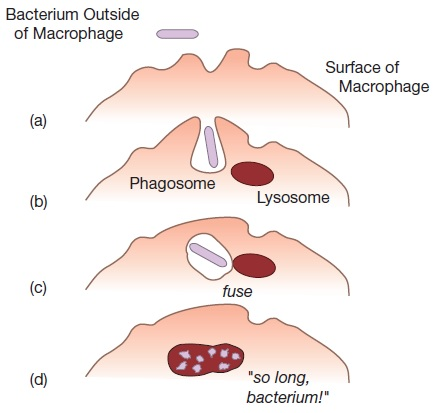
\includegraphics[width=0.5\textwidth]{1_macrofago}
	\caption{Fagocitosis.}
	\label{fig:macrofago}
\end{figure}


Durante la batalla con las bacterias, los \textit{macrófagos} producen y secretan unas proteínas llamadas \textit{citoquinas}, que facilitan la comunicación entre células del sistema inmune y que cobrarán un papel muy relevante en los capítulos que siguen.
Podríamos decir que los \textit{macrófagos} hacen el papel de centinelas, que cuando ven al enemigo mandan señales (\textit{citoquinas}) para reclutar a más defensores. A continuación, veremos otros tipos de células, en este caso referentes al \textit{sistema inmune adaptativo}.

\subsection{El sistema inmune adaptativo}
\label{sub:sistInmAdap}

El nombre es bastante descriptivo y es que gracias a este sistema somos capaces de adaptar nuestras defensas a nuevos invasores. Pero no fue hasta la década de $1790$ cuando tuvimos constancia de esta habilidad adaptativa. Por aquel entonces Edward Jenner, conocido como \textit{el padre de la inmunología}\footnote{\url{https://historia.nationalgeographic.com.es/a/edward-jenner-probablemente-cientifico-que-mas-vidas-ha-salvado-historia_14242}}, comenzó a vacunar a la población inglesa contra la viruela, que hasta entonces era una enfermedad temible. Lo que Jenner observó es que los ganaderos que se dedicaban a ordeñar vacas y que contraían el virus de la viruela bovina (\textit{cowpox}, en inglés) raramente contraían la viruela. Así que Jenner decidió llevar a cabo un experimento, poniendo en práctica el método conocido como \textit{variolización}\footnote{Este proceso consistía en inocular material infectado a una persona sana y fue introducido en Londres en 1721 por Lady Montagu, esposa del embajador inglés en Turquía.} que aprendió en el hospital de San Jorge de Londres: para ello guardó pus de uno de los ganaderos con viruela bovina y lo usó para inocular a un niño sano, James Phillips. El resultado fue una fiebre leve que desapareció a los pocos días. Después Phillips fue reinoculado con pus proveniente de una persona con viruela, pero no contrajo la enfermedad. De esta manera, Jenner demostró que el sistema inmune humano podía proporcionar armas para protegernos de un intruso que no había visto antes, ¡había inventado la vacuna! Es importante observar que la vacuna contra la viruela solo protegía contra esta enfermedad o algunas causadas por virus similares, como en el caso de la viruela bovina. Es decir, el sistema inmune adaptativo se adapta para defendernos de invasores \textit{específicos}. 

Veamos ahora en qué consiste la acción del sistema adaptativo. Para ello necesitamos hacer uso de los conceptos de \textit{antígeno} y \textit{anticuerpo}. Los \textit{anticuerpos} son proteínas específicas que el cuerpo humano es capaz de producir y que pueden adherirse a otras sustancias, externas o internas, llamadas \textit{antígenos}. La misión principal de los \textit{anticuerpos} es identificar a los \textit{antígenos} generados por un agente \textit{patógeno}, marcándolos así para su eliminación. Las células encargadas de la producción de \textit{anticuerpos} son las células B. Estas son un tipo de linfocito blanco producido en la médula que, gracias a su receptor de membrana, son capaces de identificar a los \textit{antígenos}. Cuando las células B nacen no están especializadas en la fabricación de un \textit{anticuerpo} concreto, una vez que maduran, su ADN se recombina especializando así a la célula. Una vez que la célula B se encuentra con su \textit{antígeno} desencadenante, ésta produce muchas células grandes conocidas como \textit{células plasmáticas}. Cada \textit{célula plasmática} es esencialmente una fábrica para producir \textit{anticuerpos}. 

Es decir, gracias a la presencia de \textit{anticuerpos}, otras células, como los ya conocidos \textit{macrófagos}, son capaces de identificar a los elementos que hay que destruir cuando aún se encuentran en el medio extracelular como muestra la Figura \ref{fig:macrofago_anticuerpo}. Pero... ¿qué ocurre cuando un virus ya ha entrado en una célula de nuestro cuerpo? Los \textit{anticuerpos} no pueden alcanzarlo y el virus puede dedicarse a replicarse cuanto quiera. En este momento llega el turno de las protagonistas de este trabajo, las células T. 



\begin{figure}[t]
	\centering
	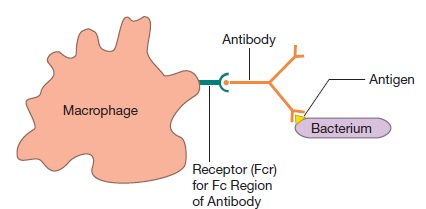
\includegraphics[width=0.6\textwidth]{2_macrofago_anticuerpo}
	\caption{Macrófago reconociendo una bacteria gracias a la acción \textit{anticuerpo-antígeno}.}
	\label{fig:macrofago_anticuerpo}
\end{figure}


\subsubsection{Las células T}
\label{Tcell}

Al igual que las células B, las células T se producen en la médula y ambas son muy similares en cuanto a su apariencia, de hecho, con un microscopio ordinario, un inmunólogo no sería capaz de diferenciarlas \citep{theHowItWorks}. La superficie de las células T también consta de unas moléculas que permiten la interacción con los \textit{antígenos} llamados receptores (TCR, \textit{T Cell Receptors}). Estos receptores permiten a estas células obtener información de su entorno y tomar decisiones en base a esa información. Por ejemplo, cuando los receptores de una célula T enlazan con un \textit{antígeno} compatible, las células proliferan para dar lugar a otras con la misma especificidad, es decir, que enlacen con el mismo \textit{antígeno}. Esta decisión de reproducción, que discutiremos con más detalle en los capítulos que siguen, es específica y lenta, tarda alrededor de una semana en completarse \citep{theHowItWorks}, lo que contrasta con la respuesta rápida que ofrece el \textit{sistema inmune innato}.

Hemos visto algunas de las similitudes que tienen las células B y T. Veamos algunas de sus diferencias: las células T maduran en el timo, de ahí la T de su nombre, mientras que las B maduran en la médula ósea. Además, las células B producen \textit{anticuerpos} que pueden reconocer cualquier molécula orgánica. Las células T, por su parte, están especializadas en el reconocimiento de un \textit{antígeno} específico y sus receptores permanecen siempre adheridos a la membrana celular y no pueden ser expulsados en forma de \textit{anticuerpo} como en el caso de las células B. Pero, quizá, la diferencia más importante sea que las células T no pueden reconocer al \textit{antígeno} ``por sí mismas'', necesitan que otra célula se lo presente \citep{theHowItWorks}. Las células que se encargan de ello se conocen como \textit{células presentadoras de antígeno}\footnote{Son macrófagos, células dendríticas, células B, entre otras.}. Las proteínas del microorganismo causante de la infección, una vez fagocitadas, son fragmentadas (formando los conocidos \textit{antígenos}) y transportadas hasta la superficie celular, donde quedan unidas a una estructura llamada \textit{complejo mayor de histocompatibilidad} (MHC) que se encuentra en la membrana de las \textit{células presentadoras de antígeno}. Gracias a su TCR las células T pueden reconocer aquellas células que han sido infectadas, puesto que el TCR y el MHC-péptido\footnote{Estructura formada por el MHC y el \textit{antígeno}.} encajan, la Figura \ref{fig:antigen_presentation} ilustra este proceso. Esta unión, si es perfecta, dura varias horas y se conoce como \textit{sinapsis inmunológica} \citep{fernandez2012mecanica}.



Hay distintos tipos de células T atendiendo al papel que desempeñan, los tres más importantes son: 
\begin{itemize}
	\item \textit{Killer o Cytotoxic T-Cells}: su misión es la de reconocer las células que han sido infectadas y, tras este proceso de reconocimiento, inducirlas al suicidio. De esta manera muere el virus, pero también la célula que había sido infectada por él. Constituyen una de las armas más potentes del sistema inmune.
	
	\item \textit{Helper T-Cells}: se encargan de regular la respuesta inmune. Una de sus tareas principales es secretar \textit{citoquinas} para controlar que la respuesta inmune sea proporcional y las células T no reaccionen de manera descontrolada.
	
	\item \textit{Regulatory T-Cells}: estas mantienen la tolerancia a \textit{antígenos} propios, previniendo la aparición de enfermedades autoinmunes.
\end{itemize}



\begin{figure}[t]
	\centering
	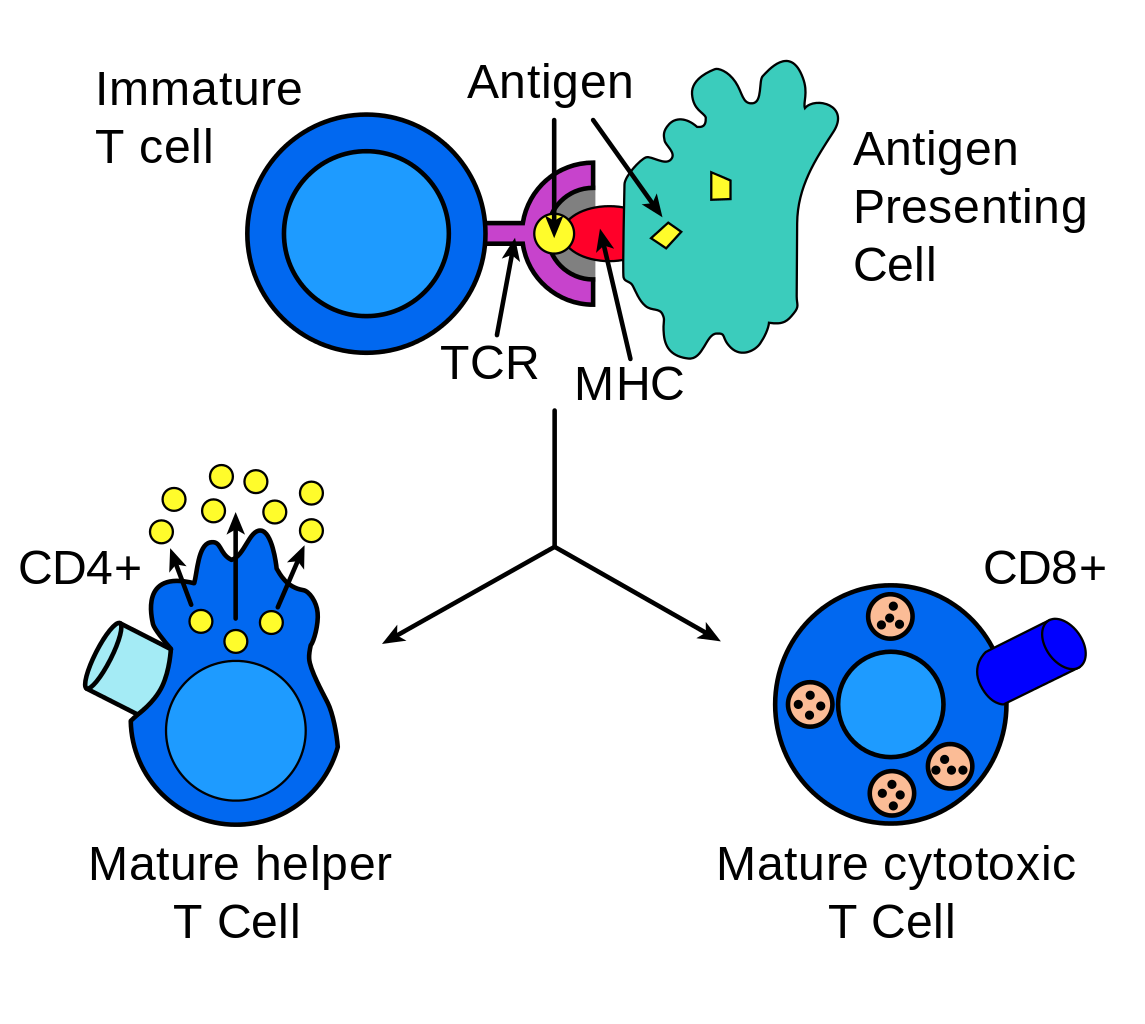
\includegraphics[width=0.6\textwidth]{Imagenes/EstadoDeLaCuestion/Antigen_presentation}
	\caption{Proceso de activación de una célula T.}
	\label{fig:antigen_presentation}
\end{figure}


Cuando las células T salen del timo se encuentran desactivadas, en un estado \textit{naïve}, y se dedican a circular por los órganos linfoides secundarios, cuyos máximos representantes son los nodos linfáticos. Allí pueden encontrarse con \textit{células presentadoras de antígeno} provenientes del foco de una infección. Si las células T reconocen al \textit{antígeno} como extraño por medio de la \textit{sinapsis inmune}, se activan, convirtiéndose así en células efectoras, capaces de secretar \textit{citoquinas} o de ir a la zona afectada a combatir la infección activamente. Una vez que las células han sido activadas, estas comienzan a proliferar masivamente, incrementando la población de células T activadas hasta en un factor de $10^6$ veces. En pocos días, las células pueden pasar por unos 15-20 ciclos de reproducción \citep{JTB}. Este proceso se conoce como \textit{expansión clonal}. Una vez que las células \textit{helper} han sido activadas pueden quedarse en los gánglios linfáticos, activando a otras células inmunitarias, o migrar al tejido infectado para secretar \textit{citoquinas} y propiciar un ambiente adecuado para controlar la infección. Por su parte, las células \textit{killer} abandonan los gánglios linfáticos para identificar aquellas células infectadas en el organismo. Cuando el \textit{patógeno} ha sido vencido, la mayoría de células T mueren, restaurando así los niveles de población iniciales (en caso contrario se acumularían millones de células que no son necesarias para el organismo) \citep{fernandez2012mecanica}. Este proceso se conoce como \textit{contracción clonal}. Sin embargo, es de gran utilidad conservar alguna de estas células experimentadas para poder reaccionar con rapidez en caso de que el mismo invasor vuelva a aparecer. Lo que hace nuestro sistema inmune es mantener un pequeño porcentaje de la población  ($5-10\%$) como células de memoria \citep{JTB}. Se llaman así porque guardan información del \textit{antígeno} contra el que combatieron. En caso de reaparición del \textit{patógeno}, estas células se activan más rápidamente y nuestro cuerpo puede así generar antes una respuesta inmune.

A lo largo de este trabajo nos centraremos en el proceso de decisión entre división o suicidio celular de una célula T durante la respuesta inmune. En la sección y los capítulos que siguen veremos cómo se ha abordado este problema desde el punto de vista matemático y las conclusiones que su estudio ha permitido obtener. 


\section{Cooperación entre dos ciencias: matemáticas y biología}
\label{sec:coop}

En esta sección trataremos brevemente la interacción entre dos ciencias muy distintas: las matemáticas y la biología, y daremos algunos ejemplos de colaboraciones y modelos matemáticos creados para reproducir e investigar distintos procesos biológicos. Nos centraremos en aquellos referidos a las células T, sobre todo al caso que nos ocupa: la dinámica de población de las mismas durante la respuesta inmune.

Después de haber seguido un desarrollo independiente durante siglos, las matemáticas y la biología han comenzado a interaccionar activamente durante los últimos años.


De hecho, los modelos matemáticos pueden llegar a ser una potente herramienta en el área de la biología. Como se puede leer en \cite{Gunawardena2014}, un modelo matemático es una máquina lógica que convierte hipótesis en conclusiones. Si el modelo es correcto y las hipótesis son ciertas entonces debemos, por lógica, creer sus conclusiones. Esta garantía lógica permite al matemático que desarrolla el modelo navegar con confianza lejos de las hipótesis y, probablemente, más lejos del lugar al que la mera intuición permite llegar. Sin embargo, no debemos confundirnos, los modelos no dan respuestas seguras. Esas respuestas son siempre consecuencia lógica de las hipótesis. En palabras de James Black\footnote{Biografía de este famoso farmacólogo: \url{https://www.britannica.com/biography/James-Black}}, los modelos matemáticos son descripciones precisas de nuestro patético pensamiento (<<\textit{accurate descriptions of our pathetic thinking}>>).

Así pues, los modelos matemáticos son herramientas en las que un biólogo se puede apoyar, pero estos modelos deben tener ciertas características para poder considerarse de utilidad por la comunidad de biólogos. A continuación, se presentan las guías que sugiere \cite{Gunawardena2014} para elaborar un buen modelo matemático:

\begin{enumerate}
	\item \textit{Formula una pregunta}. En ocasiones los modelos matemáticos no son diseñados para el avance del conocimiento de la biología, solo responden a investigaciones matemáticas que se basan, aparentemente, en problemas biológicos. Como ya se ha comentado en alguna ocasión, los modelos deben centrarse en aportar información que el biólogo desconocía. Intentar responder con un modelo a una pregunta puede ser clave a la hora de desarrollarlo con criterio, para que pueda ser juzgado por profesionales fuera del ámbito matemático. 
	
	\item \textit{Hazlo simple}. Incluir todos los procesos bioquímicos puede tranquilizar a los biólogos, pero no hará que el modelo sea mejor. De hecho, se convertirá en un modelo repleto de parámetros, poco flexible, difícil de estudiar y simular. Es mejor tener hipótesis simples y claras, intentando buscar una abstracción del problema.
	
	\item \textit{Si el modelo no puede ser refutado, entonces no está diciendo nada interesante}. No es suficiente con que el modelo reproduzca hechos observados. En muchas ocasiones el ajustar demasiado el modelo provoca que lo seleccionemos para que se ajuste a lo que queremos explicar dejando un modelo poco flexible, que apenas aporta nuevo conocimiento.
\end{enumerate}

Podemos distinguir dos tipos de estrategia en cuanto a los modelos se refiere: Modelado hacia adelante (\textit{forward modeling}) o inverso (\textit{reverse modeling}). El modelado inverso empieza con los datos experimentales, construye correlaciones entre ellos y les da estructura con un modelo matemático. Por su parte, el modelado hacia adelante empieza desde lo conocido, o sospechado, expresado en la forma de un modelo, a partir del cual se hacen predicciones. 

El modelado inverso se ha utilizado con el fin de analizar grandes volúmenes de datos genómicos y postgenómicos y, a veces, se equipara erróneamente con la biología de sistemas. Ocasionalmente ha sugerido nuevas ideas conceptuales, pero se ha utilizado con mayor frecuencia para sugerir nuevos componentes o interacciones moleculares, que luego han sido confirmados por enfoques biológicos convencionales. Los modelos en sí mismos han tenido menos importancia para comprender el comportamiento del sistema que como contexto matemático en el que la inferencia estadística se vuelve factible. En contraste, las mayores aportaciones a nuestra comprensión del comportamiento de problemas biológicos, como la homeostasis o la retroalimentación, han surgido del modelado hacia adelante. Puesto que los modelos actuales (cimentados en ecuaciones diferenciales o teoría de procesos estocásticos, por ejemplo) derivan, normalmente, de fenómenos y conocimiento conocidos. El primer beneficio que se obtiene de esto es que fuerzan al modelo a establecer unas hipótesis claras \citep{mathsModInmu}. Esto no implica que el modelado inverso no sea interesante. Hay muchas situaciones, especialmente cuando se tratan datos clínicos, donde la estructura de los datos se desconoce o es muy compleja, y las estrategias del modelado inverso cobran sentido \citep{Gunawardena2014}. 

El descubrimiento del microscopio a finales del siglo XVII provocó una revolución en la biología al revelar mundos invisibles y anteriormente desconocidos. Las matemáticas pueden ser interpretadas en la actualidad como un microscopio más general, ya que, pueden revelar mundos invisibles en todo tipo de datos, no solo ópticos. Por ejemplo, la tomografía computarizada puede revelar una sección transversal de una cabeza humana a partir de la densidad de los rayos X sin necesidad de abrir la cabeza. Charles Darwin tenía razón cuando escribió que las personas con una comprensión \textit{<<de los grandes principios principales de las matemáticas ... parecen tener un sentido adicional>>} \citep{darwin1887life}. Los biólogos de hoy reconocen cada vez más que las matemáticas pueden ayudar a interpretar cualquier tipo de datos. En este sentido, las matemáticas son el próximo microscopio de la biología\footnote{\url{https://www.ncbi.nlm.nih.gov/pmc/articles/PMC535574/}}.

\subsection{Modelos matemáticos \textit{versus} inmunología experimental}
\label{sub:modelosvsinmuno}

Como ocurre en otras ciencias, las áreas de la biología se han especializado en gran medida. Esto provoca que una mayor cantidad de detalles sea necesaria para entender los conceptos o sistemas que se estudian y que, por tanto, los modelos matemáticos, que tienden a simplificar y a hablar en términos de fórmulas y ecuaciones y, en muchos casos son difíciles de explicar, hayan sido considerados irrelevantes. En el área de la inmunología esto no es muy diferente, en \cite{mathsModInmu} se exponen algunas de las razones por las cuales los modelos matemáticos y la inmunología experimental se han mantenido separados:

\begin{enumerate}
	\item El descubrimiento de nuevos agentes y fenómenos del sistema inmune, acompañados de nueva jerga.
	
	\item El avance rápido de la tecnología y la producción de cada vez más datos.
	
	\item El contraste del entorno académico, cultura y terminología de ambas ciencias.
\end{enumerate}

Puede parecer que las dos primeras sugieren precisamente un acercamiento entre las dos ciencias. En muchos procesos biológicos, como los dinámicos, la intuición es insuficiente. Por ejemplo, las dinámicas de poblaciones son bastante complicadas de imaginar, mientras que con un modelo podemos obtener conclusiones muy precisas que nos aporten información sobre aspectos conocidos del comportamiento de la población, pero también sobre aspectos desconocidos que el modelo predice y que pueden ser probados o refutados experimentalmente. No obstante, bien es cierto que mientras que la biología sustenta su conocimiento en la experimentación, las matemáticas lo hacen sobre las pruebas rigurosas. Sin embargo, en la mayoría de los artículos relacionados con las matemáticas aplicadas a la biología las demostraciones son escasas, prevalecen las simulaciones numéricas de los modelos. Para muchos matemáticos, la calidad de un trabajo se mide en la simplicidad de formulación del problema, la dificultad de análisis y el rigor de la solución, pero estas no son siempre bien recibidas por los biólogos. Se podría decir que las colaboraciones matemático-biólogo contienen demasiadas matemáticas para este último y muy pocas para los matemáticos más teóricos \citep{RoleOfM}. AÑO DE LA PUBLICACIÓN?

A continuación, mencionaremos algunos ejemplos en los que los modelos matemáticos han aportado nuevo conocimiento al campo de la inmunología, concretamente en el estudio de las conocidas células T. 


\subsubsection{Dinámica de las células T. Decisión entre división o apoptosis}
\label{cuestionAmodelizar}

Antes de revisar los distintos trabajos que se han realizado en este ámbito, recordemos brevemente el marco conceptual en el que nos movemos. En \ref{Tcell} decíamos que cuando las células T se activan en presencia de un \textit{antígeno} estas comienzan a reproducirse rápidamente para combatir la infección y, una vez superada, muchas de ellas se suicidan restaurando los valores de población iniciales. Es lo que denominábamos respectivamente como \textit{expansión clonal} y \textit{contracción clonal}. Más aún, los experimentos realizados ponen de manifiesto que la presencia del \textit{antígeno} no es suficiente para desencadenar la decisión de división o apoptosis, ya que las células T activadas continúan reproduciéndose incluso cuando el estímulo (\textit{antígeno}) está ausente y algunas se suicidan aun cuando la infección persiste \citep{JTB}. Estos son hechos observados; lo que se desconoce es el mecanismo de decisión por el cual una célula decide dividirse o morir. Varios modelos matemáticos, desarrollados bajo diferentes hipótesis, han sido propuestos para abordar este problema. Por una parte, se ha sugerido que el proceso de activación de las células T en estado \textit{naïve} desencadena un programa que solo depende de la estimulación por \textit{antígeno} inicial. Así las cosas, una célula T efectora, por tanto, ya activada, comienza una serie de divisiones, desde un mínimo entre 7 y 10 y un máximo variable (relacionado con la estimulación por \textit{antígeno} que recibió cada célula de manera individual durante su activación). Después de estas divisiones, la célula se suicida. Bajo esta suposición, la cantidad de \textit{antígeno} que percibe una célula T en estado \textit{naïve} durante su activación determina las divisiones de todas sus células hijas. Para precisar más este modelo, se propuso que este programa pudiera estar regulado también mediante \textit{citoquinas} y no solo por la presencia de \textit{antígeno}, aunque los detalles concretos de esta regulación no son conocidos \citep{JTB}. Por otro lado, se han propuesto alternativas a este modelo basadas en procesos estocásticos. En este caso la decisión entre división o apoptosis de una célula T vendría determinada por la competición de dos relojes estocásticos. Como ocurría en el caso anterior, los procesos celulares y moleculares específicos para dilucidar este algoritmo de decisión aún están en el aire. 

A continuación, presentamos otro modelo, expuesto en \cite{JTB}, cuyas hipótesis biológicas, ecuaciones y simulaciones se desarrollan durante los dos capítulos siguientes. Es un modelo que basa la decisión de cada célula T en la concentración de \textit{antígeno} y de dos proteínas inhibidoras, Retinoblastoma (Rb) y linfoma de célula B-2 (Bcl-2), que la célula encuentra en el medio extracelular que la rodea. De esta manera, este algoritmo determinista rompe con la rigidez de los modelos mencionados anteriormente y permite que cada célula decida, en función de la información que obtiene de su alrededor, la duración de su vida, si debe dividirse o no y el momento en el que debe hacerlo. 



\chapter{Algoritmo de decisión de las células T durante la respuesta inmune}
\label{cap:descripcionTrabajo}


El modelo matemático que se presenta a continuación intenta dar respuesta al proceso biológico que vimos en la Sección \ref{cuestionAmodelizar}. A partir de unas hipótesis (procesos bioquímicos conocidos) se desarrollan una serie de ecuaciones diferenciales muy sencillas que, de hecho, pueden resolverse de manera explícita. Esta es una de las principales características del modelo, se ha intentado que este fuera lo más simple posible, reduciendo el número de parámetros al mínimo, haciendo que las simulaciones del mismo sean asequibles y más fáciles de entender. 

Estos sistemas de ecuaciones modelizan tanto la dinámica de las células T efectoras, sin olvidar las de memoria, como la dinámica del \textit{patógeno}. Recordemos que no es el único modelo que se ha propuesto para este mismo proceso biológico, en el caso que nos ocupa el modelo rompe con la idea fija que presentaban algunos otros. Esto es, la idea de que las células se dividían un número fijo de veces después de ser activadas o la idea de la competición entre relojes estocásticos de vida o suicidio celular (ver \ref{cuestionAmodelizar}). En su lugar, asumiremos en nuestro modelo que estas decisiones (división o apoptosis) vienen determinadas por la competición de dos moléculas inhibidoras: Retinoblastoma (Rb), que previene la expresión de genes necesarios para que la célula pueda continuar el ciclo celular y dividirse, y linfoma de célula B-2 (Bcl-2), que bloqueará la muerte celular. También tendremos en cuenta que la las células T se comunican con el exterior gracias a sus TCR (ver \ref{Tcell}) y, por tanto, sus decisiones se ven influenciadas por la cantidad de receptores que tengan, es decir, cuantos más receptores, más estímulos serán capaces de percibir. 

La \textit{expansión} y \textit{contracción clonal} pueden ser vistas también desde una perspectiva global como la manifestación de muchas decisiones individuales, recordemos que las células T basan sus decisiones únicamente en la información que recogen de su entorno, y, por ello, presentamos a continuación un modelo microscópico. Es decir, se modela una a una la decisión de cada célula. En el Capítulo \ref{cap:modeloMacroscopico} se propone un modelo macroscópico, que consistirá en un sistema de ecuaciones que modeliza las dinámicas viendo la población como un único sistema, es decir, en conjunto, no como decisiones individuales. Analizaremos este modelo con más profundidad y veremos que ambos modelos, macro y micro, dan resultados muy similares. 

\section{Hipótesis biológicas} 
\label{sec:hip_bio}

En lo que sigue explicaremos con detalle las tres hipótesis biológicas en las que se centra nuestro modelo. Cabe destacar que estas se basan en hechos contrastados y observados en el campo de la biología y que no constituyen, en ningún caso, la explicación al problema que se modeliza. Es decir, no son las hipótesis las que se ajustan al modelo, sino el modelo el que se basa en estos hechos.
Bien es cierto que estas hipótesis no son los únicos hechos que se conocen, pero son suficientes para la formulación de un modelo sencillo y con resultados relevantes. Como veíamos en la Sección \ref{sec:coop} es importante que el modelo tenga flexibilidad suficiente para que pueda amoldarse a mayor cantidad de situaciones. En nuestro caso, a \textit{patógenos} con distintas tasas de reproducción o células T con distintas afinidades al \textit{antígeno}, por ejemplo. 

\subsection{La competición entre dos moléculas inhibidoras determina la decisión y la duración de la vida de una célula T}
\label{subsec:hip_1}
	 
La división celular, así como, el programa de apoptosis están bloqueados al comienzo de la formación de las células T. Como ya avanzábamos en la introducción (ver Sección \ref{cap:descripcionTrabajo}), la acción de dos moléculas inhibidoras, Retinoblastoma (Rb) y linfoma de célula B-2 (Bcl-2), va a tener un papel clave no solo en la decisión entre apoptosis o división de las células T, sino también en el momento en el que deben hacerlo. Por una parte, Rb frena el inicio del ciclo celular. Para desactivar esta función y que la célula pueda dividirse, es necesario que un número suficiente de estas moléculas sea fosforilado \footnote{Fosforilación: adición de un grupo fosfato a cualquier otra molécula.}.  Por otra parte, las proteínas Bcl-2 bloquean el camino hacia la muerte celular durante infecciones agudas, mediante la contención de la acción de otras proteínas como \textit{Bax} o \textit{Bim}.


\begin{figure}[t]
	\centering
	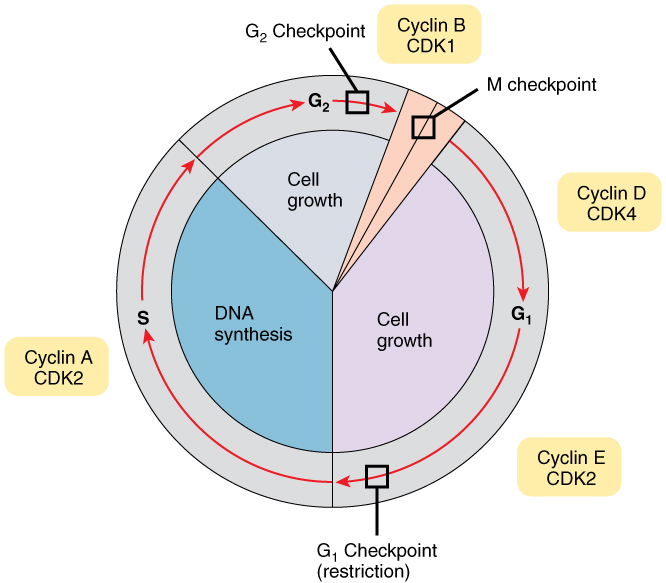
\includegraphics[width=0.5\textwidth]{Cell_Cycle}
	\caption{Representación del ciclo celular.}
	\label{fig:ciclo celular}
\end{figure}

Para nuestro modelo estableceremos que la célula pasa el \textit{punto de restricción} \footnote{El punto de restricción es el punto entre las fases $G_{1}$ y $S$, donde pasamos del crecimiento celular a la división (o apoptosis).} (ver Figura \ref{fig:ciclo celular}) si la cantidad de Bcl-2 o de Rb cae por debajo de cierto límite, dando lugar al inicio de la muerte celular o división, respectivamente. Es decir, cuando el número
de moléculas de Rb activas disminuye hasta un valor crítico, la célula abandona $G_1$ para iniciar la división celular y, cuando la cantidad de moléculas de Bcl-2 alcanza un umbral, la célula abandona $G_1$ para poner en marcha los mecanismos que llevan a la muerte celular. La variación en las dinámicas de Rb y Bcl-2 da una explicación de la variabilidad observada en la duración de la fase $G_{1}$ de las células y, consecuentemente, en la duración de sus vidas.

\subsection{Los receptores de membrana regulan las dinámicas de Rb y Bcl-2}
\label{sub:hip_recep}

La fluctuación en la cantidad de Rb y Bcl-2 depende de unas proteínas llamadas \textit{citoquinas}, que ya estudiamos en la Sección \ref{sec:cuestInmuno}. Estas pueden inducir tanto la fosforilación de Rb, en cuyo caso se denominan \textit{citoquinas de proliferación}, como tener un efecto positivo o negativo en cuanto a la cantidad de Bcl-2 se refiere, en ese caso nos referiremos a ellas como \textit{citoquinas de supervivencia} o \textit{muerte}, respectivamente.

El punto importante es que la acción que las citoquinas llevan a cabo se produce gracias sus interacciones con receptores de membrana específicos. De esta manera, el efecto que percibe una célula T depende, no solo de la cantidad de citoquinas del ambiente, sino también del número de receptores de membrana de la célula. De esta manera, si, por ejemplo, tenemos una concentración muy alta de cierta citoquina, podríamos asumir que el efecto que esta va a tener en una célula T vendrá determinado por la cantidad de receptores de membrana específicos para ella que posea la célula en cuestión. También sabemos que el número de receptores de membrana de una célula varía a lo largo de su vida, haciendo así que células adyacentes que compartan un entorno similar (la concentración de citoquinas sea la misma, por ejemplo) presenten comportamientos distintos si expresan diferentes receptores de membrana.

\subsection{Las células T naïve se dividen de manera asimétrica después de su activación.}
\label{sub:hip_divAsim}

Postulamos que tanto los fenotipos de las células T efectoras como los de las células T con memoria se determinan durante la sinapsis inmune. Esto es, una célula T en estado \textit{naïve} puede diferenciarse en una célula T efectora o en una célula T de memoria. Por su parte, una vez diferenciadas, las células T efectoras y de memoria, se dividen de manera simétrica, es decir, las células hijas heredarán el tipo la madre, y ambos tipos pueden considerarse indistinguibles durante la respuesta inmune.

\section{Modelo matemático}
\label{sec:modelo}

Basándonos en las hipótesis anteriormente formuladas proponemos a continuación una serie de ecuaciones, con variables continuas y discretas, que darán forma al algoritmo de decisión de nuestro estudio. Como ya habíamos avanzado, se trata de un modelo sencillo, tanto es el caso que los sistemas de ecuaciones diferenciales de primer orden propuestos tienen una solución explícita. Sin embargo, es esta mima sencillez lo que hace de él un modelo tan potente, pues, como veremos en el capítulo siguiente, obtenemos resultados que no solo se ajustan a los hechos observados sino que sacan a la luz comportamientos poblacionales difícilmente observables desde un laboratorio.

Antes de expresar en términos matemáticos las condiciones del modelo, damos cabida a la notación y a algunas aclaraciones previas: 

\begin{itemize}
	\item Denotaremos por \textit{$c(t)$} y \textit{$a(t)$} la cantidad de Rb y Bcl-2 activa en tiempo $t$, respectivamente.

	\item Establecemos, sin pérdida de generalidad, que los límites que determinan la decisión entre división o apoptosis (ver hipótesis \ref{subsec:hip_1}) estarán en $c(t)=0$ y $a(t)=0$, respectivamente. De acuerdo a esta hipótesis definimos: 
	
	\begin{itemize}
		\item \textit{Decisión}: Fase que parte desde el nacimiento de la célula hasta que una de las células inhibidoras alcanza el límite establecido.
		
		\item \textit{Ciclo}: Fase que se extiende desde la \textit{punto de restricción} hasta la división celular.
		
		\item \textit{Apóptosis}: Tiempo de vida de la célula que comprende desde la desactivación de Bcl-2 y la finalización del programa de muerte celular ACAD (Activated T Cell Autonomous Death).
		
		\item \textit{División}: Estado final después de que la célula haya entrado en la fase de ciclo.
		
		\item \textit{Muerte}: Estado final después de haberse completado la fase de apoptosis.
	\end{itemize}

	\item \textit{$R_{i}$} será el receptor de la i-ésima citoquina y \textit{$r_{i}(t)$} será la cantidad de ese receptor en tiempo $t$. 
	\item $r_{T}$ es el número de señales TCR/antíeno  percibidas por la célula T correspondiente.
	
	\item Los parámetros $\mu_{Tc}$ y $\mu_{Ta}$ denotan la tasa de cambio de las moléculas inhibidoras por cada señal del TCR. Mientras que los parámetros $\mu_{ic}$ y $\mu_{ia}$ representan la tasas de cambio de las moléculas inhibidoras por cada señal $R_i$.
	
	\item $\lambda_{Tj}$ es la tasa de cambio del receptor $R_{j}$ por cada señal del TCR. Mientras que $\lambda_{ij}$ es la tasa de cambio del receptor $R_j$ por cada señal $R_i$.
	
	\item $k$ es el número de receptores de membrana.
\end{itemize} 

Así las cosas, ya estamos en condiciones de presentar las ecuaciones del modelo. Como ya hemos visto en la Sección \ref{sec:hip_bio}, la dinámica de los inhibidores está controlada por las señales que recibe la célula de sus receptores de membrana durante la fase de decisión. Además, este número de señales depende del número de receptores de la célula. Si ponemos todas estas hipótesis en conjunto, llegamos a unas ecuaciones como las siguientes:

\begin{equation}
	\label{sist_inhib}
	\left\{ \begin{array}{l}
	\dot{c}(t) = \mu_{Tc}r_{T}(t) + \sum_{j=1}^{k}\mu_{jc}r_{j}(t)\\
	\dot{a}(t) = \mu_{Ta}r_{T}(t) + \sum_{j=1}^{k}\mu_{ja}r_{j}(t) \\
	\end{array}
	\right.
\end{equation}

Con el Sistema \ref{sist_inhib}, ponemos de manifiesto que las concentraciones de Rb y Bcl-2, representadas por $c(t)$ y $a(t)$, respectivamente, dependen del número de señales TCR/antígeno ($r_{T}$) y, del número de receptores de membrana que posea la célula en cuestión.

Asumimos que los receptores de membrana involucrados en el algoritmo de decisión de las células T son independientes y tienen efectos aditivos. Según la hipótesis \ref{sub:hip_recep}, asumimos que las células son capaces de ``contar'' el número de señales que llegan, cuando estas llegan a cierto número la célula se divide o se suicida. De acuerdo con estas relaciones lineales obtenemos un modelo más robusto, puesto que configuraciones similares de receptores de membrana provocarán decisiones celulares similares. 

Luego, para los receptores de membrana proponemos la siguiente ecuación: 

\begin{equation}
	\label{sist_recep}
	\begin{array}{ll}
	\dot{r}_{i}(t) = \lambda_{Ti}r_{T}(t) + \sum_{j=1}^{k}\lambda_{ji}r_{j}(t) & \mbox{para $i=1,...,k$} 
	\end{array}
\end{equation}


\subsubsection{Aspectos técnicos del modelo}

En esta breve sección damos cabida a los aspectos más técnicos, entre los que se incluyen las condiciones que marcaran en cambio de fase de una célula T, es decir, la condición que propiciará el paso de la fase de \textit{decisión} a \textit{ciclo}, por ejemplo, o los parámetros que tienen las células hijas al nacer .

\begin{itemize}
	\item Las condiciones $a(t)\geq0$, $c(t)\geq0$ y $r_i(t)\geq0$, para $i=1,...,k$ definen el domino de las ecuaciones \ref{sist_inhib} y \ref{sist_recep} durante la fase de decisión. 
	
	\item Cualquier receptor con valor negarivo $r_i(t)\leq0$ es \textit{reseteado} a 0 sin cambiar la fase de decisión en la que está la célula.
	
	\item Por su parte, las condiciones $a(t)=0$, $c(t)=0$ desencadenan el inicio de la fase de apoptosis y ciclo, respectivamente. Estas fases son excluyentes y no se pueden revertir mediante estimulación por \textit{citoquinas}. Además tienen longitud constante que denotaremos por $t_{apo}$ y $t_{cycle}$.
	
	\item Si la célula progresa en la fase de ciclo los valores de $a(t)$ y $c(t)$ deben ser reiniciados para que las células hijas puedan comenzar la fase de decisión otra vez. 
	
	\item Una vez que la célula termina la fase de apoptosis es retirada de la población.
	
	\item Los parámetros $\lambda_{ji}$, $\mu_{ic}$, $\mu_{ia}$, $\mu_{Tc}$, $\mu_{Ta}$, $c(0)$ y $a(0)$ se consideran parámetros estructurales, es decir, se refieren a procesos biológicos que permanecen constantes durante la simulación. Mientras que los parámetros referentes a la composición de receptores de membrana para una célula concreta $r_{i0}$ dependen de la historia de encuentros con el antígeno que ha tenido su madre y diferirán entre las células hijas cuando esta se divida (veremos cómo en la sección siguiente).
\end{itemize}


\section{Dinámica del patógeno durante la respuesta inmune}
\label{modeloPatCelT}

Ahora que ya tenemos un algoritmo para la dinámica de población de las células T, modelizamos la interacción del patógeno con estas células. Debemos recordar que la dinámica de un patógeno depende en gran cantidad de las características de este. Sin embargo, en esta sección daremos unas ecuaciones muy generales para que sean aplicables a la mayor cantidad posible de situaciones. En este caso, la dinámica del patógeno vendrá dada por:

\begin{equation}
	\label{sist_pat_T}
	\begin{array}{ll}
	\dot{y}(t) = \alpha y(t) - \beta n(t)y(t)
	\end{array}
\end{equation} 

Donde $y(t)$ y $n(t)$ denotan el número de células del patógeno y el número de células T, respectivamente. Los parámetros $\alpha$ y $\beta$ son positivos y dependen del antígeno: $\alpha$ representa la tasa de proliferación del patógeno, mientras que $\beta$ la tasa de eliminación del mismo a causa de las células T.

De acuerdo con este modelo, podemos ver que el patógeno aumenta su población hasta que el número de células T alcanza cierto valor, en ese momento $\dot{y}(t)$ se hace negativa y, en consecuencia, $y(t)$ comienza a decrecer. Asumiremos que las señales captadas por el TCR de una célula T son proporcionales al número de encuentros que tenga con el antígeno. Si llamamos al número de señales TCR de una célula $x$ en tiempo $t$, $r_{T}^{x}(t)$, tenemos:

\begin{equation}
	\label{ec:rhotau}
	r_{T}^{x}(t) = \gamma\rho_{n}^{x}y(t)
\end{equation}

Donde $\gamma$ es un parámetro que depende del antígeno y denota la probabilidad de que haya una activación del TCR debido a un encuentro con el antígeno. Por otro lado, $\rho_{n}^{x}$ representa la cantidad de antígeno que está disponible para una célula T, $x$, en porcentaje. Luego:

\begin{equation}
	\sum_{x=1}^{n} \rho_{n}^{x} \leq 1
\end{equation}

Según la hipótesis \ref{sub:hip_divAsim}, las células T que ya se han diferenciado se dividen de manera simétrica y reparten sus receptores de membrana entre sus dos células hijas. De esta manera, la experiencia con el antígeno, propia de cada célula puede ser transmitida a la siguiente generación.

\begin{equation}
	\label{sist:div_sim}
	\left\{ \begin{array}{l}
	r_{i0}^{1}= \delta_{i}^{x} r_{i}^{x}\\
	r_{i0}^{2}= (1-\delta_{i}^{x}) r_{i}^{x} \\
	\end{array}
	\right.
\end{equation}


Donde $\delta_{i}^{x}$ representa el ratio de receptores de membrana de tipo $R_{i}$ entre las células hijas, $r_{i0}^{1}$ y $r_{i0}^{2}$ denotan los valores iniciales de receptor $R_{i}$ en las células hijas 1 y 2, respectivamente, y  $r_{i}^{x}$ denota el número de receptores $R_{i}$ en la célula T $x$ en el momento de la división celular.



Ahora que ya hemos visto todos los conceptos matemáticos que subyacen en este modelo, estamos en condiciones de ver gráficamente los resultados que presenta y hacer el análisis correspondiente. En el capítulo siguiente veremos las simulaciones de este mismo modelo aunque un tanto simplificado, se supone que el número de receptores de membrana es dos ($k = 2$), por ejemplo. Se simularán diferentes situaciones, entre ellas: tolerancia e intolerancia al \textit{patógeno} o respuesta inmune en el caso de poblaciones de células T con distintas afinidades al patógeno. Todas estas situaciones han sido reproducidas a partir del mismo modelo, con el simple cambio del valor de sus parámetros, poniendo de manifiesto la capacidad del mismo para reproducir con facilidad situaciones diversas. 

%\section{Resumen y conclusiones}

%Antes de embarcarnos en las simulaciones de este modelo, vamos a resumir los aspectos más importantes de este capítulo con la finalidad de que el capítulo siguiente resulte más cómodo de leer.
%
%Lista de puntos clave:

%\begin{enumerate}
%	\item El algoritmo determina qué decisión, división o suicidio, toman las células T.
%	\item Las decisiones se toman de manera individual y se basan en la información que reciben del entorno a través de su TCR.
%	\item Lo que decide qué decisión se toma y cuándo es la cantidad de ciertas moléculas inhibidoras.
%	\item Ciclo y apoptosis son fases mutuamente exclusivas e irreversibles.
%	\item Cuando una célula T se divide sus hijas son del mismo tipo y comparten sus receptores de membrana.
%	\item Cuando una célula muere se elimina de la población.
%	\item El crecimiento del antígeno depende del número de células T y decrece cuando las células T comienzan a crecer.
%	\item Cuando las células T detectan al patógeno su población crece rápidamente y decrece también rápidamente cuando el patógeno ha sido vencido, aunque con cierto desfase.
%	\item En la última etapa de la respuesta inmune coexisten dos tipos de linfocitos T: los linfocitos sensibles a la apoptosis, que mueren durante la \textit{contracción clonal} (efectores), los linfocitos resistentes a la apoptosis, que	sobreviven en forma de linfocitos de memoria.
%\end{enumerate} 






\chapter{Simulaciones del modelo microscópico}
\label{cap:simulaciones}

A lo largo de este capítulo se expone en detalle cómo se han realizado las simulaciones del modelo descrito en la Sección \ref{sec:modelo}. En este caso, se han realizado algunas simplificaciones para facilitar tanto la exposición como la implementación (ver Sección \ref{sec:modelo_simplif}). En la Sección \ref{sec:implem_pseudo} se exponen algunas puntualizaciones básicas sobre la implementación de los algoritmos utilizados para las simulaciones de la Sección \ref{sec:simulacionesMicro}. Entre estas explicaciones incluyen un pseudocódigo y aclaraciones sobre aspectos concretos. La versión completa del código principal de este capítulo, realizado en Matlab, puede verse en el Apéndice \ref{Appendix:A}. Como ya se ha comentado en el capítulo anterior, es posible ajustar los parámetros del modelo de manera que se  pongan de manifiesto distintos comportamientos poblacionales. Concretamente se presentan situaciones de intolerancia al \textit{patógeno} (Sección \ref{sim:intoler}), en las que las células T terminan con la población de \textit{patógeno}, acabando así con la infección, situaciones de tolerancia (Sección \ref{sim:toler}), correspondientes al caso en el que las células T no consiguen controlar la infección y el agente que la produce se hace con el control del organismo y se discute también qué ocurre cuando poblaciones de células T con distinta afinidad a un \textit{patógeno} se enfrentan a él (Sección \ref{sim:difPoblacionesT}).

%En lo que sigue, estudiaremos el comportamiento individual de cada célula y describiremos el resultado global de las decisiones individuales de cada una de ellas. 

\section{Modelo simplificado}
\label{sec:modelo_simplif}

Para las simulaciones hemos optado por una versión simplificada del modelo propuesto en la Sección \ref{sec:modelo}, de tal manera que el número de parámetros sea suficiente para no perder la esencia del argumento pero no muy elevado para evitar distraer al lector con notación engorrosa. Siguiendo con la notación de \ref{sec:modelo}, asumiremos $k=2$. Es decir, suponemos que hay dos tipos de receptores en la membrana de nuestras células T: \textit{p} (de proliferación) y \textit{d} (de muerte) que controlan la evolución de los inhibidores de ciclo (Rb) y apoptosis (Bcl-2), respectivamente.

Distinguiremos dos tipos de células T: las efectoras, que son las que combaten activamente al \textit{patógeno}, y las de memoria, que guardan información sobre el agente infeccioso con la finalidad de dar una respuesta inmune más rápida en caso de reaparición de este agente. Cada tipo de células constituye una población distinta, pues las ecuaciones que determinan su comportamiento son distintas. Para las células T efectoras asumimos que los receptores de proliferación (\textit{p}) se expresan a partir de las señales que reciben gracias a su TCR y que, simultáneamente, autorregulan su expresión induciendo la producción de receptores tipo muerte\footnote{Esto no se produce en sentido contrario, los receptores tipo \textit{d} no activan receptores de tipo \textit{p}.} (\textit{d}). Así las cosas, las ecuaciones \ref{sist_inhib} y \ref{sist_recep} pueden escribirse como:

\begin{equation}
	\label{sist9_simplif}
	\left\{ \begin{array}{l}
	\dot{c}(t) = -\mu_{pc}p(t) \\
	\dot{a}(t) = -\mu_{da}d(t)  \\
	\dot{p}(t) = \lambda_{Tp}r_{T}(t) - \lambda_{pp}p(t) \\
	\dot{d}(t) = \lambda_{pd}p(t) \\
	\\
	c(0)=c_0 \\
	a(0)=a_0 \\
	p(0)=p_0 \\
	d(0)=d_0 
	\end{array}
	\right.
\end{equation}

%Así mismo, hemos simulado este Sistema \ref{sist9_simplif} y la Ecuación \ref{sist_pat_T} 
Para el caso de las células T de memoria hay que tener en cuenta que este tipo de células no muere durante la \textit{contracción clonal}, es por ello que las ecuaciones que regulan esta población difieren ligeramente de las vistas en el Sistema \ref{sist9_simplif}. La dinámica de las células T de memoria viene dada por el mismo Sistema \ref{sist9_simplif}, en el que se ha tenido en cuenta que $d=0$, puesto que nos centramos solamente en el inhibidor del ciclo celular y no en el de muerte. De esta manera, las ecuaciones que rigen el algoritmo de decisión para células T de memoria viene dado por: 

\begin{equation}
	\label{sist15_simplif}
	\left\{ \begin{array}{l}
	\dot{c}(t) = -\mu_{pc}p(t) \\
	\dot{p}(t) = \lambda_{Tp}r_{T}(t) - \lambda_{pp}p(t) \\
	\\
	c(0)=c_0 \\
	p(0)=p_0 \\
	\end{array}
	\right.
\end{equation}

Con estos tres sistemas de ecuaciones (Sistemas \ref{sist_pat_T}, \ref{sist9_simplif} y \ref{sist15_simplif}) queda definido el marco teórico del modelo. Sin embargo, antes de poder simular numéricamente estas ecuaciones debemos elegir los valores concretos que tomarán los parámetros. Esta no es una tarea sencilla, puesto que nadie sabe cuánto pueden valer estos parámetros en la realidad. La elección de los parámetros que hemos hecho para la primera simulación (Sección \ref{sim:intoler}) se recoge en la Tabla \ref{tabla:param}. En base a esta elección y a las variantes que se exponen a lo largo de esa sección, obtenemos unos resultados que nos permiten identificar distintos tipos de respuesta inmune, sin necesidad de invocar ningún mecanismo distinto a las hipótesis detalladas en la Sección \ref{sec:hip_bio}. A continuación se presentan algunos detalles de la implementación.


\section{Detalles de implementación y pseudocódigo}
\label{sec:implem_pseudo}

Con ánimo de aclarar algunos aspectos técnicos, se especifican, paso por paso, las instrucciones seguidas para la realización de las simulaciones. El Algoritmo \ref{algo:pseudocodigo} contiene un pseudocódigo muy sencillo con los detalles claves y prácticamente independientes del lenguaje de programación que se utilice. El código completo, realizado en Matlab, puede verse en el Apéndice \ref{Appendix:A}.

La clave principal de la implementación es cómo se guarda la población de células disponibles en cada momento. Esta información se guarda en una matriz, donde se especifica el tipo de la célula (efectora, de memoria, si está en fase de ciclo, apoptosis o decisión)\footnote{Cada una de estas fases constituye un tipo distinto. Por ejemplo, una célula T efectora puede ser de tipo $1$ si está en fase de decisión, $3$ si está en fase de división o $4$ si está en fase de apoptosis.}, la cantidad de Rb y Bcl-2 que tiene disponible a su alrededor, el número de receptores de membrana que tiene y el tiempo que le queda para finalizar la fase correspondiente. Como se trata de un modelo microscópico, en el que cada célula toma su decisión de manera independiente, el hilo conductor de la implementación se basa en recorrer la matriz de células y ejecutar la decisión tomada por la célula que se esté tratando. Cada vez que se recorre la población de células T asumimos que pasa un tiempo $t_{next}$ que actualiza el tiempo actual de la simulación al final de la iteración y que permite determinar cuándo una célula ha acabado la fase de división o apoptosis. Una vez establecidas las estructuras necesarias para guardar la información, veamos las instrucciones concretas del modelo.

\begin{enumerate}
	\item Comenzamos la simulación en un tiempo inicial $t=0$ y acabamos en un tiempo final $T_{final}$ configurable.
	
	\item Para cada tiempo $t$, se calcula la cantidad de \textit{patógeno} disponible, $Y$. 
	
	\item En función de $Y$, y para cada célula T de la población, se calcula la cantidad de \textit{patógeno} que está a su alcance y se resuelve el sistema de ecuaciones correspondiente para conocer la cantidad de Rb ($c$) y Bcl-2 ($a$) activa en ese instante. En función de esto se desencadenará la división celular, si $c = 0$, o el suicidio de la célula, si $a = 0$. En otro caso la célula seguirá en fase de decisión y volverá a calcular $a$ y $c$ en la siguiente iteración en base a la cantidad obtenida en la actual.
	
	\item Si la célula va a dividirse se generan dos células hijas con los parámetros correspondientes al TCR, recordemos que la cantidad de receptores de la célula madre se divide entre las dos hijas de manera asimétrica, y los parámetros iniciales, para que pueda comenzar su fase de \textit{decisión}. Se sigue en el paso 6.
	
	\item Si por el contrario la célula comete suicidio, se eliminará de la población. 

	\item Se contempla la siguiente célula de la población y se vuelve a 3.
	
	\item Se actualiza el tiempo para la siguiente iteración y se vuelve a 1.
\end{enumerate}


\begin{algorithm}
	\caption{Algoritmo de la decisión. Células T.}
	\label{algo:pseudocodigo}
	\begin{algorithmic}[1]
		
		% ENTRADA / SALIDA
		
		\State Inicialización de parámetros según \ref{tabla:param}
		\State $t = 0;$ \Comment{t será el tiempo por el que vamos simulando}
		
		\While{ $t\ < \ T_{final}$}
		  
		\State $Y = Y_{init}*e^{t*(\alpha - N*\beta)};$ \Comment{Calculamos Y con la solución explícita de \ref{sist_pat_T}}
		
		\For{$nCell; nCell++; N$} \Comment{Para cada célula T de la población}
			\State $ r_{T}=\rho*Y;$ \Comment{Ecuación \ref{ec:rhotau}}
			\If{$efectora(nCell)$} \Comment{Si es una célula T efectora}
				\State Se resuelve \ref{sist9_simplif}
				\If{$a \leq 0 $}
					\State La célula $nCell$ se elimina de la población
				\ElsIf{$c \leq 0$}
					\State La célula $nCell$ se divide
					\State Las condiciones iniciales de las células hijas vienen determinadas por $a_0, c_0$ y \ref{sist:div_sim}
				\EndIf
			
			\ElsIf{$memoria(nCell)$} \Comment{Si es una célula T de memoria}
				\State Se resuelve \ref{sist15_simplif}
				\If{$c \leq 0$}
					\State La célula $nCell$ se divide siguiendo el mismo procedimiento que la división de una célula T efectora. 
				\EndIf
			\EndIf
		\EndFor
		
		\State $t = t + t_{next};$
		\State Se actualiza el número de células de la población.	
		
		\EndWhile
		
	\end{algorithmic}
\end{algorithm}

En este pseudocódigo se ha detallado cuáles son las ecuaciones involucradas en cada paso. A continuación, exponemos algunas particularidades de la simulación: hemos omitido que cuando las condiciones son $a > 0$ y $c > 0$, en el caso de las células T efectoras y $c > 0$, en el caso de las células T de memoria, la célula permanece en la fase de decisión pero actualiza sus condiciones para la siguiente iteración según los resultados que ha obtenido en la iteración actual. También hay que tener en cuenta que la división celular y el proceso de apoptosis no se llevan a cabo de manera inmediata, conllevan un tiempo $t_{cycle}$ y $t_{apo}$, respectivamente, por lo que el número total de células en la población debe actualizarse una vez que estos procesos hayan finalizado y no instantáneamente, como pueden sugerir las líneas $10$, $12$ y $17$ del pseudocódigo. Otro aspecto que hemos supuesto es que el parámetro $\gamma$ que aparecía en la Ecuación \ref{ec:rhotau} es $\gamma = 1$. Es decir, suponemos que todo encuentro del TCR de la célula T con el antígeno va a desencadenar una activación. El parámetro $\rho$ debe ser calculado de tal manera que todas las células T tengan las mismas posibilidades a la hora de \textit{obtener su parte de \textit{patógeno}}, en la implementación real se usó un vector de números aleatorios entre $0$ y $1$ normalizado por el número total de células T. Buena parte de la notación usada en el Algoritmo \ref{algo:pseudocodigo} ya ha sido introducida a lo largo de este trabajo, pero volvemos a insistir en que $Y$ representa el número de moléculas del \textit{patógeno}, mientras que $N$ la cantidad total de células T, incluyendo las efectoras y las de memoria. Sin embargo, en la implementación real, en la línea $4$ del pseudocódigo, el $N$ utilizado es solamente el número total de células T efectoras, sin contar las de memoria\footnote{Esto se ha hecho así porque el proceso que siguen las células T de memoria es más complejo que lo que se recoge en el modelo. Estas células al cabo de un tiempo se desactivan y para que tengan un efecto sobre el \textit{patógeno} deben volver a activarse. Para intentar hacer el modelo lo más sencillo posible se ha optado por hacer que las únicas células que combaten al \textit{patógeno} sean las T efectoras.}.


\begin{table}[h]
	\begin{center}
		\begin{tabular}{>{\centering\arraybackslash}m{2cm} >{\arraybackslash}m{3cm} >{\arraybackslash}m{7cm} }%{|l|l|l|}
			\hline
			\multirow{9}{*}{} & $t_{cycle} = 0.15$               & Duración de la fase de ciclo.                             \\ \cline{2-3}
			& $t_{apo} = 0,2$                  & Duración de la fase de apoptosis.                         \\ \cline{2-3}
			& $t_{next} = 0,3$                 & Duración del paso en la simulación.                       \\ \cline{2-3}
			& $a_0 = 0,3$                      & Cantidad inicial de Bcl-2 para células T efectoras.       \\ \cline{2-3}
			Variables         & $c_0 = 0,08$                     & Cantidad inicial de Rb para células T efectoras.          \\ \cline{2-3}
			& $c_0^{mem} = 0,04$               & Cantidad inicial de Rb para células T de memoria.         \\ \cline{2-3}
			& $N_{ini} = 25$                   & Número inicial de células T naïve.                        \\ \cline{2-3}
			& $Y_{ini} = 5$                    & Número inicial de moléculas del \textit{patógeno}.                 \\ \cline{2-3}
			& $r_p, r_d = 0$                   & Número inicial de receptores de membrana $p$ y $d$.       \\ \hline
			\multirow{2}{*}{Patógeno}  & $\alpha = 6$                    & Tasa de proliferación.                                    \\ \cline{2-3}
			& $\beta = 0,04$                    & Tasa de muerte por linfocito.                             \\ \hline
			\multirow{5}{*}{} & $\lambda_{pd} = 0,05$            & Tasa de cambio del receptor $R_d$ por cada señal $R_p$.   \\ \cline{2-3}
			& $\lambda_{Tp} = 6*10^{-5}$       & Tasa de cambio del receptor $R_p$ por cada señal del TCR. \\ \cline{2-3}
			Células T  efectoras       & $\lambda_{pp} = 0,5*10^{-4}$     & Tasa de cambio del receptor $R_p$ por cada señal $R_p$.   \\ \cline{2-3}
			& $\mu_{pc} = 15$                 & Tasa de cambio de Rb por cada señal del TCR.              \\ \cline{2-3}
			& $\mu_{da} = 10$                 & Tasa de cambio de Bcl-2 por cada señal del TCR.           \\ \hline
			\multirow{4}{*}{} & $\lambda_{Tp}^{mem} = 10^{-5}$   & Igual que $\lambda_{Tp}$, para células T de memoria.      \\ \cline{2-3}
			Células T de memoria        & $\lambda_{pp}^{mem} = 2*10^{-2}$ & Igual que $\lambda_{pp}$, para células T de memoria.      \\ \cline{2-3}
			& $\mu_{pc}^{mem} = 13$           & Igual que $\mu_{pc}$, para células T de memoria.          \\ \cline{2-3}\hline
		\end{tabular}
		\caption{Tabla de variables y parámetros.}
		\label{tabla:param}
	\end{center}
\end{table}

\section{Resultados y análisis}
\label{sec:simulacionesMicro}

En esta sección expondremos los resultados de las simulaciones realizadas. Comenzaremos discutiendo dos situaciones básicas que se pueden dar en una infección: que las células inmunes logren controlar la infección o que, por el contrario, sea el agente infeccioso el que acabe tomando el control de nuestro organismo, y acabaremos mostrando el resultado de diversas simulaciones cuando la afinidad por el \textit{patógeno} de las células T va variando.

\subsection{Intolerancia al \textit{patógeno}}
\label{sim:intoler}

Se entiende como situación de intolerancia al \textit{patógeno} aquella en la que las células T son capaces de controlar la infección y eliminar por completo al agente infeccioso. La simulación correspondiente a este caso puede verse en la Figura \ref{fig:intolerance}. En la figura se puede observar que el \textit{patógeno}, representado con un línea roja, crece rápidamente, debido a la elección de una tasa de crecimiento, $\alpha$, elevada. Una vez que las células T son conscientes de la rápida proliferación de un agente no deseado, su número comienza a crecer. Sin embargo, como ya habíamos comentado anteriormente, esto se produce con cierto retraso tras la aparición del \textit{patógeno}. Lo que estamos describiendo es la conocida \textit{expansión clonal}. Este crecimiento de células T provoca que el término que acompaña a $\beta$ en la Ecuación \ref{sist_pat_T} comience a ser más grande que el acompañado por $\alpha$ en esta misma ecuación, causando así que la derivada de $y$ se haga negativa y, por tanto, el número de células del \textit{patógeno} comience a decrecer. Debemos mencionar que el número de células T necesarias para eliminar al \textit{patógeno} viene regulado por el parámetro $\beta$ (siempre que el resto de parámetros permanezcan inalterados), si este fuera más grande, es decir, las células T fueran más dañinas con el \textit{patógeno}, el número de células T necesarias para controlar la infección sería menor (y viceversa).

%veríamos una curva azul con un máximo mas pequeño que el de la Figura \ref{fig:intolerance}. (EN REALIDAD EN ESTA FIGURA LA GRÁFICA ESTÁ NORMALIZADA, SERÍA MEJOR PONER LA OTRA SIN NORMALIZAR?)

Prestemos atención ahora al comportamiento de las células T de memoria: por la sección anterior, ya sabíamos que las células T efectoras y las de memoria iban a constituir poblaciones distintas, puesto que las ecuaciones que rigen sus dinámicas son distintas. La principal diferencia es que las células T de memoria no se suicidan una vez el \textit{patógeno} ha desaparecido, permanecen con la información necesaria para atacar al \textit{patógeno} más rápidamente en caso de reaparición. En la Figura \ref{fig:intolerance} vemos cómo estas células de memoria aumentan su población tras la aparición del \textit{patógeno}, aunque se produce un crecimiento tan rápido ni elevado como en el caso de las T efectoras. Su población queda reducida a un $5-10\%$ de la población de células T.

\begin{figure}[t]
	\centering
	\begin{tabular}{cc}
		\subfloat[Simulación: caso de intolerancia al \textit{patógeno}. Los parámetros son los expuestos en la Tabla \ref{tabla:param}.]{
			\label{fig:intolerance}
			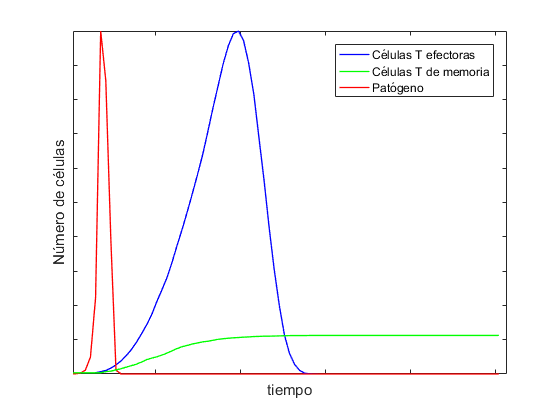
\includegraphics[width=0.5\textwidth]{Imagenes/Simulaciones/intolerance}}
		& \subfloat[Simulación: caso de tolerancia al \textit{patógeno}. Los parámetros son los mismos que se exponen en la Tabla \ref{tabla:param}, excepto: $\alpha = 1$, $\beta = 0.01$, $\mu_{pc} = 3$, $\mu_{da} = 2$, $\mu_{pc}^{mem} = 2$.]{
			\label{fig:tolerance}
			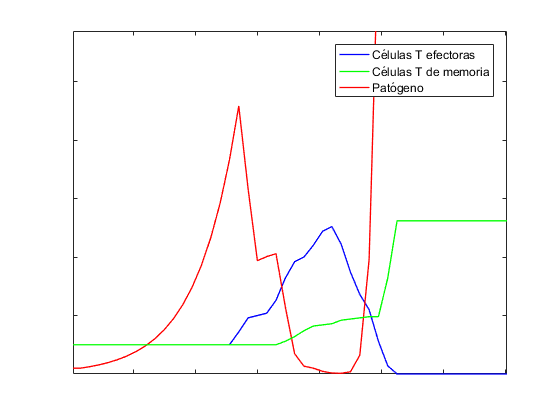
\includegraphics[width=0.5\textwidth]{Imagenes/Simulaciones/tolerance}}\\
	\end{tabular}
	\caption{Simulaciones del modelo microscópico. Casos de tolerancia e intolerancia al \textit{patógeno}}%\label{foo}
\end{figure}

%\begin{figure}[t]
%	\centering
%	%\begin{tabular}{c}
%		\subfloat[Simulación: caso de intolerancia al \textit{patógeno}. Los parámetros son los expuestos en la Tabla \ref{tabla:param}.]{
%			\label{fig:intolerance}
%			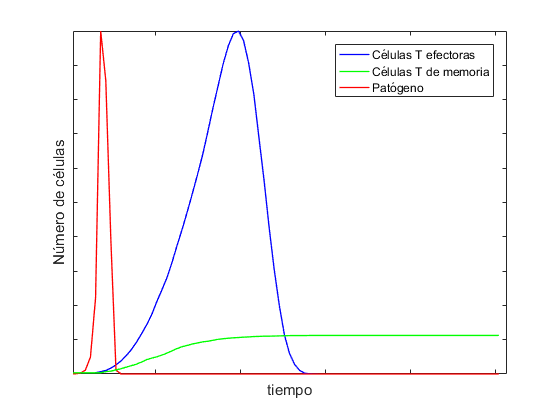
\includegraphics[width=0.7\columnwidth]{Imagenes/Simulaciones/intolerance}}
%		
%		\subfloat[Simulación: caso de tolerancia al \textit{patógeno}. Los parámetros son los mismos que se exponen en la Tabla \ref{tabla:param}, excepto: $\alpha = 1$, $\beta = 0.01$, $\mu_{pc} = 3$, $\mu_{da} = 2$, $\mu_{pc}^{mem} = 2$.]{
%			\label{fig:tolerance}
%			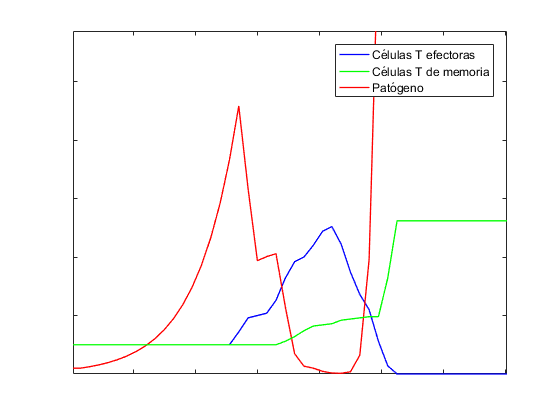
\includegraphics[width=0.7\columnwidth]{Imagenes/Simulaciones/tolerance}}\\
%	%\end{tabular}
%
%	\caption{Simulaciones del modelo microscópico. Casos de tolerancia e intolerancia al \textit{patógeno}}%\label{foo}
%\end{figure}


%\begin{figure}[t]
%	\centering
%	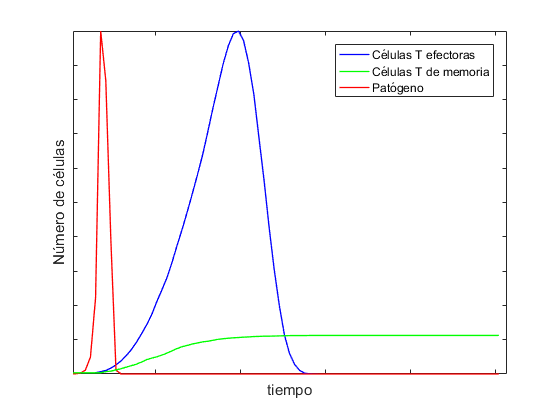
\includegraphics[width=0.7\textwidth]{Imagenes/Simulaciones/intolerance}
%	\caption{Simulación: caso de intolerancia al \textit{patógeno}. Los parámetros son los expuestos en la Tabla \ref{tabla:param}.}
%	\label{fig:intolerance}
%\end{figure}

\subsection{Tolerancia al \textit{patógeno}}
\label{sim:toler}

Hemos visto en la sección anterior una simulación de intolerancia al \textit{patógeno}. Esto es, las células inmunes consiguen controlar la infección y erradicar por completo al agente infeccioso. Sin embargo, esto no es siempre así. Existen \textit{patógenos}, como la bacteria \textit{Mycobacterium Tuberculosis}\footnote{\url{https://www.omicsonline.org/open-access/why-is-mycobacterium-tuberculosis-hard-to-grow-the-principle-of-biorelativity-explains-2161-0681.1000176.php?aid=26260} \\ \url{https://www.britannica.com/science/bacteria/Growth-of-bacterial-populations}}, que han desarrollado una estrategia que consiste en crecer a un ritmo muy lento. De esta manera \textit{sigilosa} engañan a las células T, haciéndolas creer que su población ha sido erradicada y provocando que estas células inmunes se suiciden  \citep{leggett2017growth}.

Como se puede ver en la Figura \ref{fig:tolerance}, las células T comienzan la \textit{expansión clonal} como respuesta a la presencia de \textit{patógeno}, al igual que en el caso anterior. Este aumento de población inmune hace que la población del \textit{patógeno} se vea afectada rápidamente (recordemos que su factor de crecimiento, $\alpha$, es pequeño en este caso) y caiga hasta niveles muy bajos. Es entonces cuando las células inmunes perciben que el \textit{patógeno} ha sido eliminado con éxito y comienzan la \textit{contracción clonal}, haciendo que su población baje hasta desaparecer. Sin embargo, debido a que el \textit{patógeno} no ha sido erradicado por completo y, ahora que la población de células T ha iniciado su fase de \textit{apoptosis}, puede reproducirse sin problema, dando lugar al crecimiento exponencial que vemos en la Figura \ref{fig:tolerance}. En poco tiempo estos \textit{patógenos} \textit{astutos} pueden tomar el control del organismo. 

En cuanto a las células T de memoria, vemos como crecen con la presencia del \textit{patógeno}. Una vez que la población de células T efectoras llega a cero el número de estas células se estabiliza, puesto que las células T de memoria no continúan reproduciéndose en ausencia de células T efectoras, a pesar de la presencia de \textit{patógeno}. Esto se debe a que las células T de memoria necesitan señales de proliferación para reproducirse y estas son generadas por las células T efectoras. 

%\begin{figure}[t]
%	\centering
%	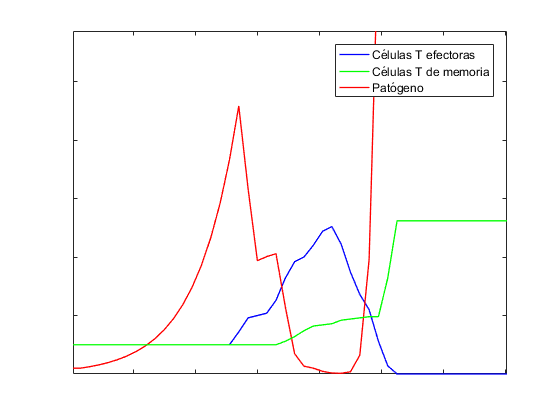
\includegraphics[width=0.7\textwidth]{Imagenes/Simulaciones/tolerance}
%	\caption{Simulación: caso de tolerancia al \textit{patógeno}. Los parámetros son los mismos que se exponen en la Tabla \ref{tabla:param}, excepto: $\alpha = 1$, $\beta = 0.01$, $\mu_{pc} = 3$, $\mu_{da} = 2$, $\mu_{pc}^{mem} = 2$.}
%	\label{fig:tolerance}
%\end{figure}

\subsection{Simulaciones con distintas poblaciones de células T}
\label{sim:difPoblacionesT}

En esta sección veremos cómo se comportan distintas poblaciones de células T efectoras frente a un mismo \textit{patógeno}. Estas poblaciones están diseñadas para que tengan afinidades distintas con el \textit{patógeno}. Además veremos cómo se comportan estas poblaciones cuando la población \textit{inmunodominante} desaparece.

Comencemos mirando la Figura \ref{fig:tresClones}. En esta simulación hemos considerado tres poblaciones con distinta afinidad, $\lambda_{Tp}$, al \textit{patógeno}. Tenemos el clon $0$ con la afinidad más alta y el clon $2$ con la más baja. La diferencia en cuanto a expansión es considerable, la población más afín al \textit{patógeno} es la que se reproduce a mayor velocidad y se denomina \textit{población inmunodominante}. Este hecho es consecuencia de las ecuaciones del Sistema \ref{sist9_simplif}: la ecuación $\dot{p}(t) = \lambda_{Tp}r_{T}(t) - \lambda_{pp}p(t)$ propicia un mayor crecimiento cuanto más alto es el valor $\lambda_{Tp}$, puesto que provoca que la derivada de $c$ se haga más negativa y se llegue antes al límite $c = 0$ que desencadena la división celular.

%\begin{figure}[t]
%	\centering
%	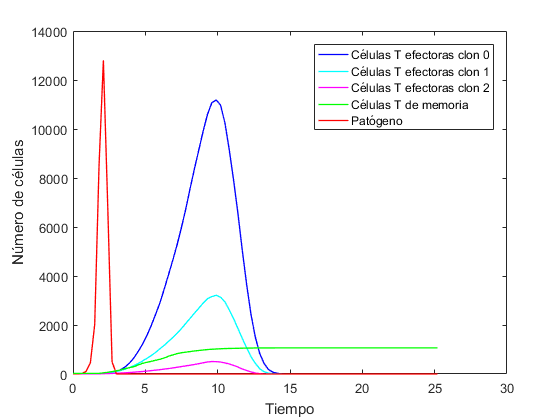
\includegraphics[width=0.7\textwidth]{Imagenes/Simulaciones/tresClones}
%	\caption{Simulación: distintas poblaciones de células T con distintas afinidades al \textit{patógeno}. Los parámetros son los mismos que se exponen en la Tabla \ref{tabla:param}, excepto: $\lambda_{Tp}^{clon_0} = 2*10^{-4}$, $\lambda_{Tp}^{clon_1} = 6*10^{-5}$, $\lambda_{Tp}^{clon_2} = 10^{-5}$.}
%	\label{fig:tresClones}
%\end{figure}


Pero... ¿qué pasaría si esta \textit{población inmunodominante} desapareciera? Una posible explicación nos la da la Figura \ref{fig:dosClones}. En ella, podemos ver que el modelo sugiere que las \textit{poblaciones subdominantes} se expanden más que antes para suplir la ausencia de la \textit{inmunodominante} y controlar la infección. No debemos olvidar que la afinidad que tienen estas poblaciones al \textit{patógeno} es menor y esto hace que este pueda crecer más en el mismo periodo de tiempo.


%\begin{figure}[t]
%	\centering
%	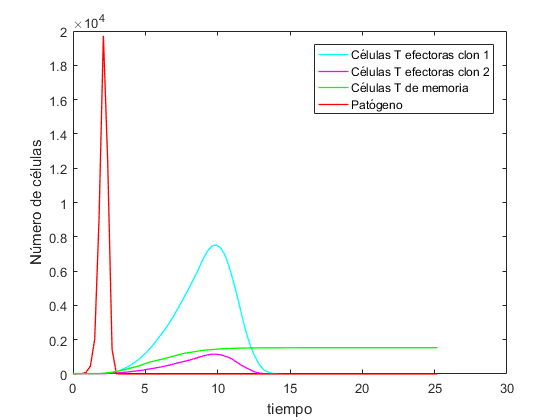
\includegraphics[width=0.7\textwidth]{Imagenes/Simulaciones/dosClones}
%	\caption{Simulación: distintas poblaciones de células T con distintas afinidades al \textit{patógeno}. Clones subdominantes. Los parámetros son los mismos que se exponen en la Tabla \ref{tabla:param}, excepto: $\lambda_{Tp}^{clon_1} = 6*10^{-5}$, $\lambda_{Tp}^{clon_2} = 10^{-5}$.}
%	\label{fig:dosClones}
%\end{figure}

Para finalizar veamos el comportamiento del clon $2$ cuando el resto de clones han desaparecido. Como es de esperar, ocurre algo similar a lo que veíamos en la Figura \ref{fig:dosClones}. En este caso el clon $2$ debe hacer un esfuerzo mayor (reproducirse más) para mantener la infección controlada. Comportamiento ilustrado en la Figura \ref{fig:unClon}.

Estas simulaciones ponen de manifiesto la importancia de las células T de memoria. En una situación donde las células T efectoras no presentan una afinidad al \textit{patógeno} muy elevada las consecuencias pueden ser muy graves, pues la infección se alarga y las células T no son suficientemente dañinas para el agente externo. Sin embargo, si contamos con células T de memoria que guardan información relevante para combatir a ese agente, nuestro organismo se encontrará en una situación más segura, ya que se podrá actuar más rápidamente con células que disponen de alta afinidad con el \textit{patógeno} y desencadenarán, por tanto, un ataque mucho más efectivo.

%\begin{figure}[t]
%	\centering
%	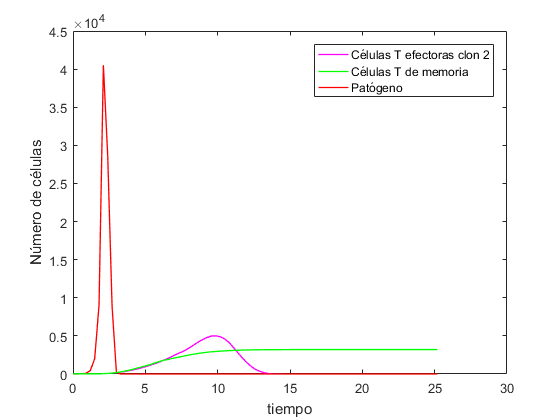
\includegraphics[width=0.7\textwidth]{Imagenes/Simulaciones/unClon}
%	\caption{Simulación: distintas poblaciones de células T con distintas afinidades al \textit{patógeno}. Clon subdominante. Los parámetros son los mismos que se exponen en la Tabla \ref{tabla:param}, excepto: $\lambda_{Tp}^{clon_2} = 10^{-5}$.}
%	\label{fig:unClon}
%\end{figure}


\begin{figure}[t]
	\centering
	%\begin{tabular}{c}
	\subfloat[Simulación: distintas poblaciones de células T con distintas afinidades al \textit{patógeno}. Clones subdominantes. Los parámetros son los mismos que se exponen en la Tabla \ref{tabla:param}, excepto: $\lambda_{Tp}^{clon_1} = 6*10^{-5}$, $\lambda_{Tp}^{clon_2} = 10^{-5}$.]{
		\label{fig:tresClones}
		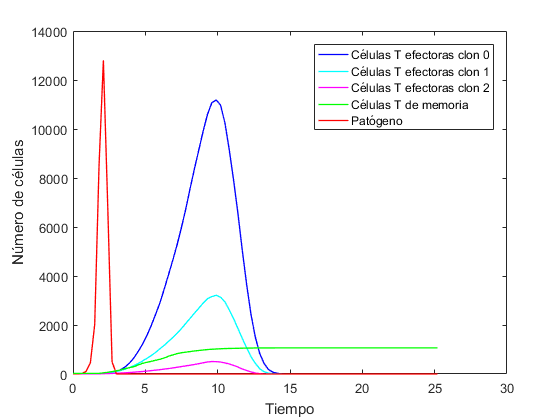
\includegraphics[width=0.5\columnwidth]{Imagenes/Simulaciones/tresClones}}
	
	\subfloat[Simulación: distintas poblaciones de células T con distintas afinidades al \textit{patógeno}. Clones subdominantes. Los parámetros son los mismos que se exponen en la Tabla \ref{tabla:param}, excepto: $\lambda_{Tp}^{clon_1} = 6*10^{-5}$, $\lambda_{Tp}^{clon_2} = 10^{-5}$.]{
		\label{fig:dosClones}
		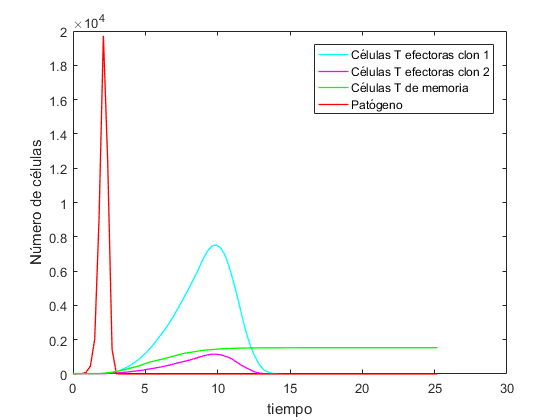
\includegraphics[width=0.5\columnwidth]{Imagenes/Simulaciones/dosClones}}\
	
	\subfloat[Simulación: distintas poblaciones de células T con distintas afinidades al \textit{patógeno}. Clon subdominante. Los parámetros son los mismos que se exponen en la Tabla \ref{tabla:param}, excepto: $\lambda_{Tp}^{clon_2} = 10^{-5}$.]{
		\label{fig:unClon}
		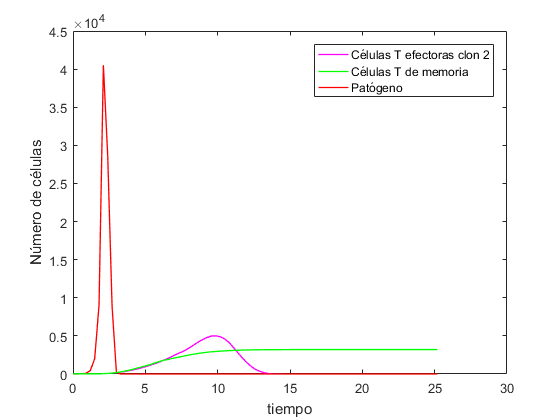
\includegraphics[width=0.5\columnwidth]{Imagenes/Simulaciones/unClon}}\\
	
	\caption{Simulaciones del modelo microscópico. Casos de tolerancia e intolerancia al \textit{patógeno}}%\label{foo}
\end{figure}


\chapter{Modelo macroscópico para la dinámica de población de las células T durante la respuesta inmune.}
\label{cap:modeloMacroscopico}

En este capítulo se expone otro modelo matemático propuesto para determinar el algoritmo de decisión entre división o apoptosis de las células T durante una respuesta inmune (ver Sección \ref{cuestionAmodelizar}). En este área aún son muchas las cuestiones que quedan por resolver: una vez que las células se activan, ¿hasta cuándo continúan dividiéndose?, ¿es esta decisión totalmente dependiente de las condiciones que hayan tenido las células en el momento de su activación?, ¿por qué hay un retraso respecto a la desaparición del \textit{patógeno} en la \textit{contracción clonal}?... Estas cuestiones se atajaron en el Capítulo \ref{cap:descripcionTrabajo}, donde se establece la base teórica de un modelo matemático a nivel microscópico. Es decir, este modelo proporciona el algoritmo de decisión para cada célula, pues las decisiones de las células inmunes son, \textit{a priori}, independientes unas de otras (no se ha encontrado un órgano que regule estos mecanismos \citep{arias2016emergent}).

En este capítulo lo que haremos será volver sobre este mismo problema pero desde una perspectiva un poco distinta, desde un punto de vista macroscópico. Esto quiere decir que las ecuaciones diferenciales sobre las que se basa el modelo determinan el comportamiento de toda la población de células. Para entender esto podemos poner como ejemplo los movimientos de un equipo de fútbol: la estrategia de contraataque del equipo vista desde el punto de vista <<macroscópico>> sería recuperar el balón y avanzar rápidamente al campo del adversario para marcar gol. Sin embargo, si nos fijamos ahora en el mundo <<microscópico>> de cada jugador, vemos que cada uno tiene su papel, defender y recuperar la posesión, pasar a los centrales o a los delanteros, etc.

%Al comienzo de este capítulo, en la Sección \ref{sec:toler_tasaCrecim}, se aborda la relación entre el caso de tolerancia al \textit{patógeno} y la tasa de crecimiento de este. Por su parte la Sección \ref{sec:iner_elast} desgrana las dos características poblacionales, incercia y la elasticidad, sobre las que se sustenta el modelo. En la última sección (Sección \ref{sec:simu_macro}), se realizan simulaciones de este modelo y se comparan los resultados con los del modelo microscópico.

Al comienzo de este capítulo, la Sección \ref{sec:iner_elast} desgrana las dos características poblacionales, incercia y la elasticidad, sobre las que se sustenta el modelo y se detallan las ecuaciones que rigen la dinámica de población de las células T y del \textit{patógeno}. En la sección siguiente (Sección \ref{sec:simu_macro}), se realizan simulaciones de este modelo y se comparan los resultados con los del modelo microscópico.


%\section{Tolerancia y tasa de crecimiento}
%\label{sec:toler_tasaCrecim}

%La respuesta inmune adaptativa se basa en la capacidad que tienen las células T para identificar diferentes \textit{antígenos} pero ¿cómo saber cuáles de ellos son amigos y cuáles enemigos? En esta sección asumiremos que las células T toleran células cuyas tasas de crecimiento permanezcan por debajo de cierto límite, es decir, aquellas que no crezcan con mucha rapidez (las células que crecen muy rápidamente se asocian con toxinas o células tumorales, por ejemplo \citep{arias2015growth}). Además, nos centraremos en dos características de la dinámica de población de las células T: la elasticidad (la población se expande y se contrae, lo conocemos como \textit{expansión} y \textit{contracción clonal}) y la inercia (la \textit{contracción clonal} se presenta con retraso tras la desaparición del \textit{patógeno}) \citep{arias2015growth}. Este resultado permite dar una posible explicación al hecho paradójico de que aquellos \textit{patógenos} que se reproducen más lentamente en un organismo sean tolerados por las células inmunes.


\section{Inercia y elasticidad en las células T}
\label{sec:iner_elast}


Como ya se avanzaba en la introducción de este capítulo, nos centraremos en dos características de la dinámica de población de las células T: la elasticidad (la población se expande y se contrae, lo conocemos como \textit{expansión} y \textit{contracción clonal}) y la inercia (la \textit{contracción clonal} se presenta con retraso tras la desaparición del \textit{patógeno}) \citep{arias2015growth}. En base a estas dos propiedades, se detallan las ecuaciones que dan lugar a este modelo matemático. El modelo consta de un sistema de ecuaciones diferenciales de segundo orden. Este tipo de ecuaciones constituye la manera más simple de representar la inercia de la población \citep{arias2015growth}. Además, las ecuaciones de segundo grado son el marco general para las dinámicas \textit{newtonianas}. Esto nos lleva a modelar de manera natural la dinámica de las células T efectoras como el balance entre dos fuerzas opuestas actuando sobre la población: una fuerza por parte del \textit{antígeno} causada por la presencia del \textit{patógeno} y una fuerza intrínseca elástica que devuelve a la población a su estado inicial. En concreto, asumiremos que la fuerza que ejerce el \textit{antígeno} es proporcional al número de células del \textit{patógeno} y modelaremos la elasticidad mediante la \textit{Ley de Hooke}, que establece que la fuerza necesaria para restablecer el equilibrio una vez que la población ha llegado a cierto valor es proporcional a dicho valor \citep{arias2015growth}. También asumiremos que el \textit{patógeno} prolifera con un ratio constante y que serán eliminados por la acción de las células T de manera proporcional a sus encuentros mutuos. De esta manera, presentamos el siguiente modelo:

\begin{equation}
	\label{sist_macro}
	\left\{ \begin{array}{l}
	{T^{\prime\prime}}(t) = -kT(t) + \lambda P(t) \\
	{P^{\prime}}(t) = \alpha P(t) - \beta T(t)P(t) \\
	\\
	T(0)=0 \hspace{3cm} ,para\, T \geq 0,\, P \geq P_m \\
	T^{\prime}(0)=0  \\
	P(0)=P_0 \geq P_m  \\ 
	\end{array}
	\right.
\end{equation}

Donde $T(t)$ y $P(t)$ son el número de células T efectoras y el número de células de \textit{patógeno}, respectivamente. La primera ecuación diferencial que nos encontramos nos sugiere que, en ausencia de \textit{patógeno}, la población de células T se puede caracterizar por una respuesta elástica en forma de soluciones oscilatorias. Así mismo, la presencia de \textit{patógeno} tendría el efecto de una fuerza externa. Siguiendo con la segunda ecuación, observamos que, en ausencia de células T, la población de \textit{patógeno} crece de manera exponencial. Sin embargo, una vez que las células T entran en acción empiezan a eliminar al \textit{patógeno} de acuerdo a posibles encuentros entre $T(t)$ y $P(t)$ \citep{arias2016emergent}. La eficiencia de cada proceso se mide en base a cuatro parámetros y las condiciones iniciales del sistema. Estos parámetros son $\alpha$, $\beta$, $k$ y $\lambda$. Los dos primeros representan la tasa de crecimiento del \textit{patógeno} y la tasa de eliminación del mismo a causa de las células T, respectivamente. Por su parte $k$ y $\lambda$ representan las constantes de elasticidad e inercia de la población, respectivamente. Una diferencia entre este modelo y otras teorías propuestas para el caso de la tolerancia inmune es que la percepción del ratio de crecimiento del \textit{antígeno} viene determinado como una propiedad general a toda la población. Mientras la decisión de activación puede ser tomada por células T en estado \textit{naïve} en base a la información local sobre las \textit{células presentadoras de antígeno}, el momento en el que comienza la \textit{contacción clonal} no puede ser establecido por ninguna célula T. Cada célula T tiene una información muy limitada acerca de la progresión de una respuesta inmune y es improbable que una célula T pueda medir, de manera individual, el ratio de crecimiento de las células que presentan ese mismo \textit{antígeno}. Sin embargo, propiedades colectivas como la inercia o la elasticidad pueden permitir a la población de células T distinguir entre una respuesta aguda o la tolerancia al \textit{patógeno} \citep{arias2015growth}.

El Sistema \ref{sist_macro} también puede expresarse de manera adimensional, reduciendo el número de parámetros a dos: 

\begin{equation}
	\label{sist_macro_nod}
	\left\{ \begin{array}{l}
	{T^{\prime\prime}}(t) = -T(t) + P(t) \\
	{P^{\prime}}(t) = \alpha^{*} P(t) - \beta^{*} T(t)P(t) \\
	\\
	T(0)=0 \hspace{3cm} ,para\, T \geq 0,\, P \geq P_m^{*} \\
	T^{\prime}(0)=0  \\
	P(0)=1 \\ 
	\end{array}
	\right.
\end{equation}

Donde $\alpha^{*} = \frac{\alpha}{\sqrt k}$, $\beta^{*} = \frac{\beta \lambda P_0}{k \sqrt k}$ y $P_{m}^{*} = \frac{P_m}{P_0}$.

En lo que sigue veremos el comportamiento de estos dos sistemas mediante una serie de simulaciones numéricas, pues en este caso las ecuaciones no tienen una solución explícita.

\section{Simulaciones del modelo macroscópico}
\label{sec:simu_macro}

A continuación presentaremos distintas situaciones que se pueden dar con la simple variación de los parámetros del modelo macroscópico visto en la sección anterior. Para poder comparar estos resultados, se simulan las situaciones de tolerancia e intolerancia vistas en el Capítulo \ref{cap:simulaciones} para el modelo microscópico y veremos cómo los parámetros $\alpha^{*}$ y $\beta^{*}$ del Sistema \ref{sist_macro_nod} nos revelan la dependencia crucial que tienen sobre el modelo en estas dos situaciones.

El código referente a esa sección puede verse en el Apéndice \ref{Appendix:A}.

%\begin{figure}[t]
%	\centering
%	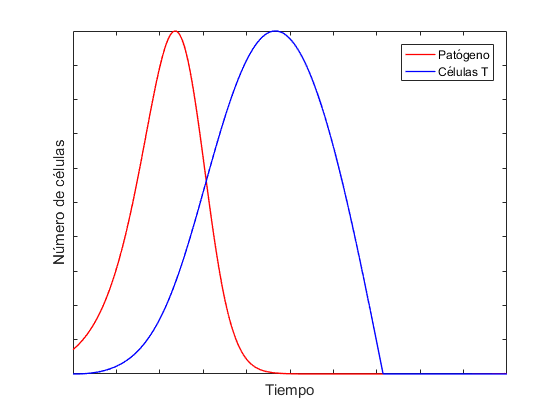
\includegraphics[width=0.7\textwidth]{Imagenes/Simulaciones/macro_intoler}
%	\caption{Simulación: caso de intolerancia al \textit{patógeno} en el modelo macroscópico.\\Parámetros: $\alpha=1,5$, $\beta=0,1$, $k=4$, $\lambda=0.5$, $P_m = 0$.}
%	\label{fig:macro_intolerance}
%\end{figure}


\subsection{Intolerancia al \textit{patógeno}}
\label{sub:simMacroIntoler}

Como vimos en la Sección \ref{sim:intoler}, el caso de intolerancia al \textit{patógeno} se da cuando las células inmunes consiguen eliminar al agente que causa la infección. 
En este tipo de simulaciones vemos como el \textit{patógeno} aumenta su población seguido de una rápida proliferación de las células T (\textit{expansión clonal}), cuya acción erradica al \textit{patógeno}. Posteriormente a la desaparición del \textit{patógeno}, y con cierto retraso, tiene lugar la \textit{contracción clonal}, que restaura los niveles de población de células T. En la Figura \ref{fig:macro_intolerance}, correspondiente a a simulación del Sistema \ref{sist_macro}, podemos ver esta situación gráficamente. 

Queda, por tanto, de manifiesto la característica de inercia, pues se ve cómo las células T comienzan a disminuir en número tiempo después de que el \textit{patógeno} haya desaparecido, y de elasticidad, pues la población de células T acaba recuperando sus niveles iniciales. Como vemos, el parecido de esta figura con la Figura \ref{fig:intolerance} es notable, ambos modelos, macroscópico y microscópico, simulan el mismo comportamiento desde dos puntos de vista distintos.


\begin{figure}[h]
	\centering
	\begin{tabular}{cc}
		\subfloat [Simulación: caso de intolerancia al \textit{patógeno} en el modelo macroscópico. Parámetros: $\alpha=1,5$, $\beta=0,1$, $k=4$, $\lambda=0.5$, $P_m = 0$.]{
			\label{fig:macro_intolerance}
			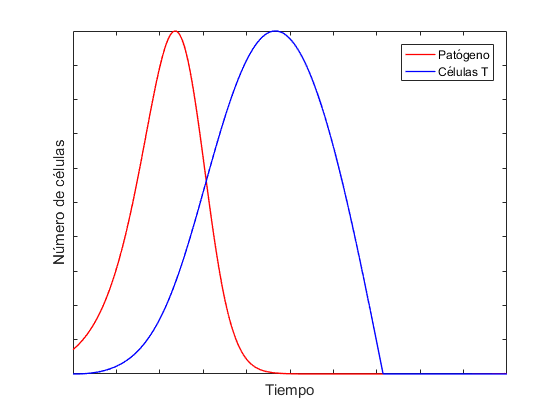
\includegraphics[width=0.5\textwidth]{Imagenes/Simulaciones/macro_intoler}}
		& \subfloat[Simulación: caso de tolerancia al \textit{patógeno} en el modelo macroscópico. Parámetros: $\alpha^{*}=1,1$, $\beta^{*}=0,01$, $P_m^{*} = 0$.]{
			\label{fig:macro_tolerance}
			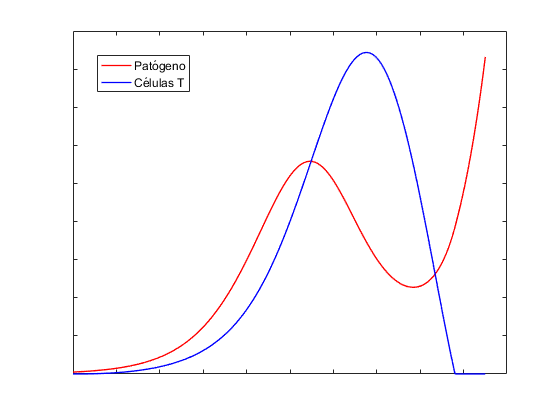
\includegraphics[width=0.5\textwidth]{Imagenes/Simulaciones/macro_toler}}\\
	\end{tabular}
	\caption{Simulaciones del modelo macroscópico. Casos de intolerancia y tolerancia al \textit{patógeno}}%\label{foo}
\end{figure}

\subsection{Tolerancia al patógeno}
\label{sub:simMacroToler}

Veamos ahora al caso análogo a la Sección \ref{sim:toler}, donde vimos cómo un \textit{patógeno} con una tasa de reproducción pequeña conseguía zafarse de las células T. En la Figura \ref{fig:macro_tolerance} puede observarse que las células T comienzan la \textit{contracción clonal}, haciendo que su población desaparezca irremediablemente, y provocando que el \textit{patógeno} pueda reproducirse sin ningún tipo de impedimento, ya que no desaparece, simplemente se reproduce más lento. En este caso la simulación corresponde al Sistema \ref{sist_macro_nod}.

%\begin{figure}[t]
%	\centering
%	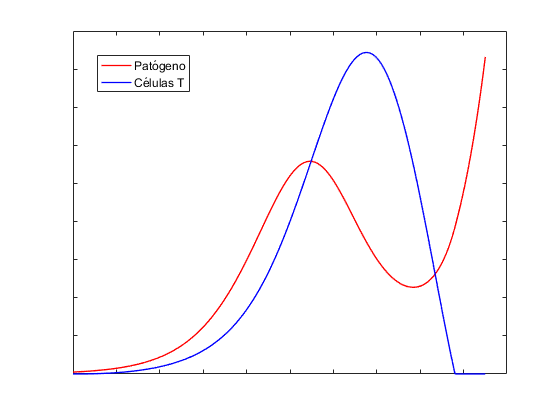
\includegraphics[width=0.7\textwidth]{Imagenes/Simulaciones/macro_toler}
%	\caption{Simulación: caso de tolerancia al \textit{patógeno} en el modelo macroscópico.\\Parámetros: $\alpha^{*}=1,1$, $\beta^{*}=0,01$.}
%	\label{fig:macro_tolerance}
%\end{figure}



\subsection{Regiones de tolerancia e intolerancia}
\label{sub:reg_tolerIntolerMacro}

Un análisis interesante que se puede hacer es determinar qué relación existe entre el valor de los parámetros del modelo y las regiones de intolerancia y tolerancia. Este asunto se ha abordado para el modelo macroscópico adimensional (ver Sistema \ref{sist_macro_nod}). Para ello se ha implementado un programa que recorre los valores de $\alpha^{*}$ y $\beta^{*}$ entre $0,1$ y $2,5$ con un paso de $0,1$\footnote{Con paso nos referimos al valor del incremento del parámetro en cada iteración.}, y, para cada valor, simula el Sistema \ref{sist_macro_nod}. Una vez hecha la simulación se observa el número de células T y de \textit{patógeno} para obtener el resultado de tolerancia, en caso de que las células T no consiguen acabar con el \textit{patógeno} o intolerancia en caso contrario. La Figura \ref{fig:macro_toler_intoler} recoge el resultado de todas estas simulaciones, arrojando datos importantes: si dejamos uno de los dos parámetros fijos, es posible cambiar de una región a otra con tan solo modificar el otro parámetro. De hecho, de acuerdo con este modelo, \textit{patógenos} y tumores pueden escapar de la acción de las células T por dos métodos: reduciendo el efecto de las células T, el parámetro $\beta^{*}$, o reduciendo su tasa de proliferación, el parámetro $\alpha^{*}$, \citep{arias2016emergent}. Una consecuencia que se puede extraer de esto es que mecanismos como la fiebre, que incrementa la tasa de proliferación del \textit{patógeno}, o la inflamación, que aumenta la acción de las células T, favorecen que el \textit{patógeno} sea vencido. 

\begin{figure}[t]
	\centering
	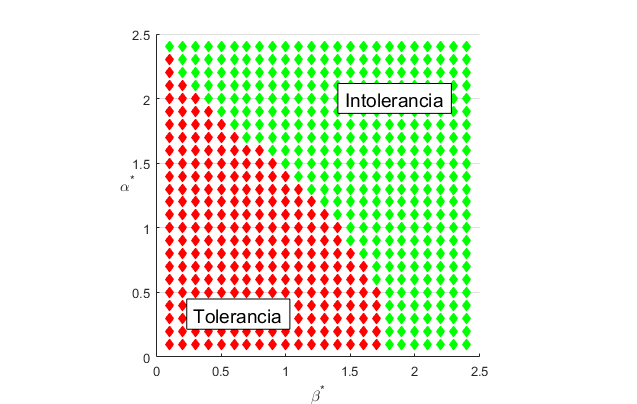
\includegraphics[width=0.8\textwidth]{Imagenes/Simulaciones/macro_toler_intoler}
	\caption{Simulación: variación de los parámetros $\alpha^{*}$ y $\beta^{*}$ para dar lugar a regiones de tolerancia e intolerancia en el modelo macroscópico adimensional.}
	\label{fig:macro_toler_intoler}
\end{figure}
\chapter{Correspondencia de parámetros entre los modelos microscópico y macroscópico}
\label{cap:redNeuronal}

En los Capítulos \ref{cap:descripcionTrabajo} y \ref{cap:modeloMacroscopico} se establece el marco teórico de dos modelos matemáticos que dan una posible explicación del mecanismo que rige la dinámica de población de las células T durante una infección aguda. Como se puede ver en las simulaciones correspondientes de estos modelos (ver Capítulo \ref{cap:simulaciones} y Sección \ref{sec:simu_macro}) ambos pueden reproducir comportamientos similares, como son el de tolerancia e intolerancia al patógeno. Sin embargo, ambos modelos son notablemente distintos por dos razones: 

\begin{enumerate}
	\item El punto de vista desde el cual se aborda el algoritmo de decisión de las células T es distinto. Mientras que el modelo microscópico describe el algoritmo de comportamiento de cada célula de manera individual, el macroscópico propone unas ecuaciones que gobiernan sobre toda la población de células. 
	
	\item Las ecuaciones diferenciales que conforman el modelo microscópico son de primer orden y su significado, desde el punto de vista biológico, está bien definido. En concreto, los parámetros de este modelo, tales como el número de receptores de membrana de la célula ($r_{i}$) o la tasa de cambio de estos receptores ($\lambda_{xy}$) (ver Tabla \ref{tabla:param}), representan conceptos biológicos claros. Por su parte, el modelo macroscópico utiliza un sistema de ecuaciones de segundo grado, basado en las dinámicas newtonianas y en dos propiedades de la población: la elasticidad y la inercia. Los parámetros $k$ y $\lambda$ representan estas dos últimas propiedades en las ecuaciones, respectivamente. Sin embargo, desde el punto de vista biológico, el valor de estos parámetros tiene un significado meramente fenomenológico y su justificación experimental es una cuestión abierta.
	 
\end{enumerate}

A pesar de que el número de parámetros del modelo macroscópico es considerablemente menor, la elección de los parámetros $k$ y $\lambda$ es más compleja que la de los parámetros del modelo microscópico por la razón $2$. Así las cosas, lo ideal sería poder establecer una correspondencia entre los parámetros de ambos modelos. De esta manera se podrían establecer los valores de los parámetros del modelo microscópico, que tienen un significado biológico claro, e inferir el valor de los parámetros del modelo macroscópico o viceversa. A lo largo de este capítulo se detalla cómo se ha abordado un aspecto concreto de este problema mediante el uso de técnicas de inteligencia artificial (Sección \ref{sec:conjDatos_entreRed}) y se interpretan los resultados obtenidos (Sección \ref{sec:resultadoRed}). 


\section{Conjunto de datos y entrenamiento de la red neuronal}
\label{sec:conjDatos_entreRed}

Como una primera aproximación a esta cuestión de correspondencia de parámetros, se propone la implementación de una red neuronal, cuyo propósito es predecir el valor de los parámetros que se le deben asignar al modelo macroscópico teniendo como entrada aspectos característicos de una simulación. En otros términos, se podría decir que se busca hacer la función inversa del modelo. Una vez hecho lo anterior, podemos hacer una simulación con unos parámetros concretos del modelo microscópico, extraer los puntos clave de la misma, y obtener el valor de los parámetros del modelo macroscópico que se deberían usar para lograr un resultado similar. 

Antes de poder implementar la red es necesario determinar con qué datos se va a trabajar. Más concretamente se deben establecer las entradas y las salidas que tendrá la red. En nuestro caso, nos limitaremos al estudio del siguiente caso particular.


\begin{itemize}
	\item Las simulaciones que se realizan para obtener los datos pertinentes se corresponden con situaciones de intolerancia al patógeno.
	
	\item La red neuronal consta de diez datos de entrada y cuatro de salida. Los seis primeros datos de entrada se corresponden con seis puntos de interés de cada simulación. Estos puntos son: el máximo número de células de patógeno alcanzado, el máximo número de células T alcanzado, el tiempo en el que se obtuvieron ambos y el tiempo en el que desaparecieron ambas poblaciones (en la Figura \ref{fig:red_micro} pueden verse destacados los puntos mencionados), que denominaremos como \textit{max\_P}, \textit{max\_T}, \textit{t\_max\_P}, \textit{t\_max\_T}, \textit{t\_min\_P}, \textit{t\_min\_T}, respectivamente. Los cuatro restantes datos de entrada son los parámetros $\alpha$, $\beta$, $k$ y $\lambda$ del modelo macroscópico con los cuales se han obtenido los seis valores anteriores. Por último, los cuatro parámetros de salida de la red se corresponden con los valores de los parámetros $\alpha$, $\beta$, $k$ y $\lambda$ predichos por la misma.
	
	\item El rango de valores para $\alpha$, $\beta$, $k$ y $\lambda$ se estableció con ayuda del modelo macroscópico adimensional (ver Figura \ref{fig:macro_toler_intoler}), para ajustarnos lo más posible a una situación de intolerancia, y de tal manera que el número de simulaciones resultantes no fuera demasiado elevado, pero permitiendo suficiente variabilidad en los datos para abarcar el mayor número posible de situaciones. En concreto, se establecieron los siguientes rangos:
	
	\begin{itemize}
		\item $\alpha \in  [0,75;7]$
		\item $\beta \in [0,1;5]$
		\item $k, \lambda \in [0,1;2]$
	\end{itemize}
	
	Con estos rangos y a un paso\footnote{Con paso nos referimos al valor del incremento del parámetro en cada iteración.} de $0,5$ se obtienen unas $2080$ simulaciones aproximadamente, de las cuales $1587$ fueron casos de intolerancia. Los valores correspondientes a los puntos de interés de la simulación y sus parámetros se recogen en el archivo \textit{data\_neural\_network\_csv} por filas y en el mismo orden que han sido mencionados (\textit{max\_P}, \textit{max\_T}, \textit{t\_max\_P}, \textit{t\_max\_T}, \textit{t\_min\_P}, \textit{t\_min\_T}, $\alpha$, $\beta$, $k$ y $\lambda$). Este documento da lugar al conjunto de datos de la red.
	
	\subsection{Aspectos técnicos de la red}
	
	Una red neuronal está compuesta por un conjunto de neuronas interconectadas entre sí mediante enlaces. Cada neurona toma como entradas las salidas de las neuronas de las capas antecesoras, cada una de esas entradas se multiplica por un peso, se agregan los resultados parciales\footnote{Se suman las entradas multiplicadas por sus pesos asociados.} y mediante una función de activación se calcula la salida. Esta salida es a su vez es entrada de la neurona a la que precede. En la Figura \ref{fig:esquemaRed1} se ilustra la estructura de una red con dos capas ocultas (\textit{hidden layer}), una capa de entrada (\textit{input layer}) y otra de salida (\textit{output layer}). Todas ellas son capas densas, es decir, están totalmente conectadas. En la Figura \ref{fig:esquemaRed2} podemos ver el esquema de cada neurona o nodo.
	
	En nuestro caso, la red cuenta con cinco capas densas y activaciones \textit{ReLu}\footnote{$ReLu(x) = max(0,x)$} (Esto es importante en la última capa, puesto que los parámetros no pueden tomar valores negativos). Como es habitual para el entrenamiento de una red neuronal, el $70\%$ del conjunto de los datos, tomado de forma aleatoria, se utilizó para el entrenamiento y el $30\%$ restante para \textit{testear} la red\footnote{Entrenar una red neuronal consiste en ajustar cada uno de los pesos de las entradas de todas las neuronas que forman parte de la red neuronal, para que las respuestas de la capa de salida se ajusten lo más posible a los datos que conocemos. \textit{Testear} una red neuronal consiste en observar cómo se comporta la red cuando los datos que tiene como entrada son distintos a los datos de entrada recibidos durante el entrenamiento. En esta fase los pesos de la red son los hallados tras el entrenamiento.}. La implementación de la red está realizada en Python y el código correspondiente puede verse en el archivo \textit{redNeuronal\_modeloMacro.py}. 
	

	
	


	\begin{figure}[t]
		\centering
		\begin{tabular}{cc}
			\subfloat[Esquema de una red neuronal con cuatro capas densas.]{
				\label{fig:esquemaRed1}
				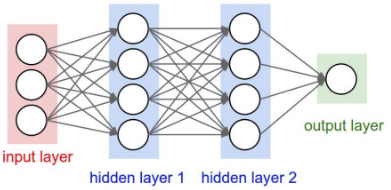
\includegraphics[width=0.5\columnwidth]{Imagenes/RedNeuronal/esquema}}
			& \subfloat[Esquema de un nodo de una red neuronal.]{
				\label{fig:esquemaRed2}
				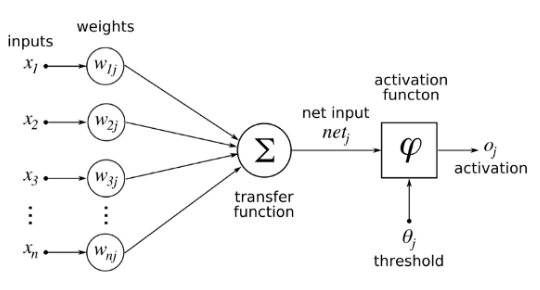
\includegraphics[width=0.5\columnwidth]{Imagenes/RedNeuronal/esquema2}}\\
		\end{tabular}
		\caption{Representación esquemática de una red neuronal.}
		\label{fig:esquemaRed}
	\end{figure}
	
	
\end{itemize}



\section{Resultados obtenidos por la red neuronal}
\label{sec:resultadoRed}

En esta sección se exponen los resultados obtenidos tras el entrenamiento de la red. Además, veremos un ejemplo real de la inferencia de parámetros dada por la red tras establecer como entrada una simulación del modelo microscópico. 

Comencemos definiendo los conceptos de \textit{epoch}, \textit{loss} y \textit{accuracy} para una red neuronal. Se entiende por \textit{epoch} cada pasada completa por todo el conjunto de datos de entrenamiento. Las redes neuronales, cuando entrenan, hacen varias pasadas por los datos y, en cada una de ellas, intentan minimizar una función de error. El concepto de \textit{loss} está asociado a esto último, pues este es el valor que intentamos minimizar. Cuanto más pequeño es, más precisas son las predicciones de la red. En nuestro caso, el valor de \textit{loss} se corresponde con el error cuadrático medio. Por su parte, el valor de \textit{accuracy} es una métrica utilizada para medir el rendimiento del algoritmo. Este valor se calcula una vez la red se ha entrenado y han fijado todos sus parámetros. El valor de \textit{accuracy} mide cómo de preciso es el modelo comparado con los datos reales. Por ejemplo, supongamos que tenemos $1000$ muestras y nuestro modelo es capaz de clasificar bien $990$ de ellas entonces, el valor de \textit{accuracy} es del $99\%$.

\begin{figure}[t]
	\centering
	\begin{tabular}{cc}
		\subfloat[Valores de \textit{loss} calculados para la red neuronal durante el entrenamiento.]{
			\label{fig:loss}
			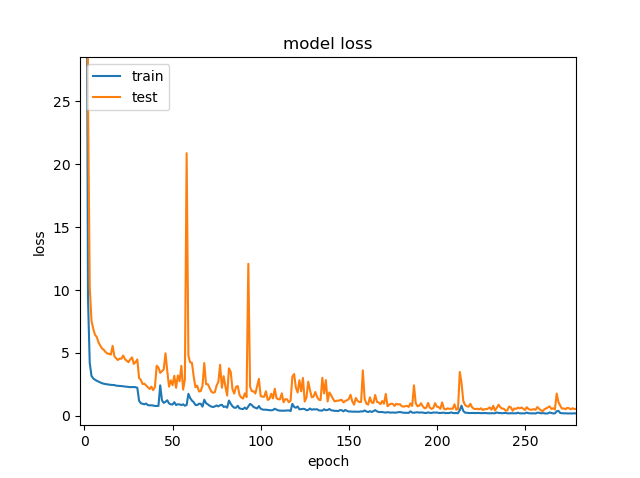
\includegraphics[width=0.5\columnwidth]{Imagenes/RedNeuronal/loss}}
		& \subfloat[Valores de \textit{accuracy} calculados para la red neuronal durante el entrenamiento.]{
			\label{fig:accuracy}
			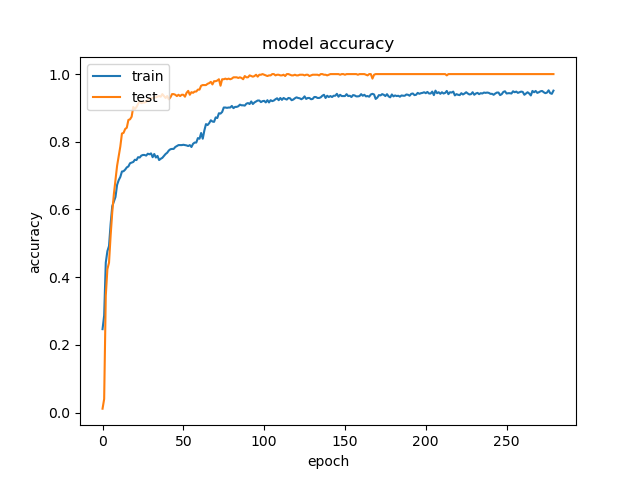
\includegraphics[width=0.5\columnwidth]{Imagenes/RedNeuronal/accuracy}}\\
	\end{tabular}
	\caption{Representación gráfica de los valores de \textit{loss} y \textit{accuracy} para cada \textit{epoch} durante el entrenamiento de la red.}
	\label{fig:loss_accuracy}
\end{figure}

En la Figura \ref{fig:loss_accuracy} podemos ver las gráficas correspondientes a los valores de \textit{loss} y \textit{accuracy} durante el entrenamiento de la red. Como se puede observar en la Figura \ref{fig:loss}, el valor de \textit{loss} consigue estabilizarse al mínimo en el conjunto de prueba una vez pasada la iteración $230$ (ver Figura \ref{fig:loss}). Por su parte, el valor de \textit{accuracy} (ver Figura \ref{fig:accuracy}) continúa incrementándose para el conjunto de entrenamiento hasta prácticamente la última iteración, lo que indica que el modelo no está sobreentrenando, a pesar de que en el conjunto de prueba se estabilice una vez pasada la iteración $100$ aproximadamente. Estos resultados sugieren que el número de \textit{epoch} utilizados para entrenar la red es el óptimo.



En el archivo \textit{resultados.txt} se pueden ver algunos de los resultados obtenidos por la red, correspondientes a distintos valores de \textit{accuracy}\footnote{El resultado de cada de las distintas simulaciones se representa por filas con el siguiente formato: [los seis puntos de interés generados tras una simulación del modelo macroscópico] $=>$ [el valor predicho por la red para los parámetros $\alpha$, $\beta$, $k$ y $\lambda$] (expected [el valor real de dichos parámetros]).}. 


\subsection{Ejemplo de ejecución de la red}

En el caso que nos ocupa ahora, detallaremos un ejemplo concreto obtenido a partir de los datos de una simulación del modelo microscópico, cumpliendo así con el propósito de esta red. En la Figura \ref{fig:red_micro} podemos ver el resultado de la simulación del modelo microscópico, con los seis puntos de interés destacados. Concretamente el valor de esos parámetros es: $\textit{max\_P} = 74,4$, $\textit{max\_T} = 88$, $\textit{t\_max\_P} = 3,15$, $\textit{t\_max\_T} = 4,8$, $\textit{t\_min\_P} = 3,9$ y $\textit{t\_min\_T} = 6,3$. Una vez la red estaba entrenada se introdujeron estos valores como entrada para obtener la predicción de los valores de los parámetros del modelo macroscópico. El resultado obtenido fue: $\alpha = 3,5$, $\beta = 0,29$, $k = 0,3$ y $\lambda = 0,9$. En la Figura \ref{fig:red_macro} puede verse la simulación del modelo macroscópico correspondiente a esos parámetros. Si comparamos ambas figuras observamos a simple vista que ambas presentan dos situaciones muy similares, si bien es cierto que los valores difieren ligeramente. En particular, la simulación del modelo macroscópico tiene en puntos de interés los siguientes valores: $\textit{max\_P} = 68.94$, $\textit{max\_T} = 98,82$, $\textit{t\_max\_P} = 1,27$, $\textit{t\_max\_T} =4$, $\textit{t\_min\_P} = 2,45$ y $\textit{t\_min\_T} = 6,87$. Si contrastamos estos valores con los obtenidos con el modelo microscópico vemos que el valor \textit{max\_P} es menor en el modelo microscópico pero que los tiempos asociados a este (\textit{t\_max\_P} y \textit{t\_min\_P}) también lo son. Esto nos dice que, a pesar de que los valores no han sido exactos, la forma de la gráfica sí se preserva. Si prestamos atención a los valores referentes a las células T, vemos que el patrón ha cambiado, pues se alcanza un número mayor de células T en el modelo macroscópico y, sin embargo, este valor se alcanza antes que en el modelo microscópico. Esto nos indica que los parámetros de elasticidad e inercia no se han ajustado completamente, lo que hace que observemos ese pequeño desfase.



\begin{figure}[t]
	\centering
	\begin{tabular}{cc}
		\subfloat[Simulación: caso de intolerancia al patógeno en el modelo microscópico. Parámetros y variables: $t\_cycle = 0,05$, $t\_apo = 0,1$, $t\_next = 0,15$, $\alpha = 6,4$, $\beta = 0.22$, $\lambda_{pd} = 0.05$, $\lambda_{Tp} = 6*10^{-5}$, $\lambda_{pp} = 0,5*10^{-4}$, $\mu_{pc} = 8$, $\mu_{da} = 15$.]{
			\label{fig:red_micro}
			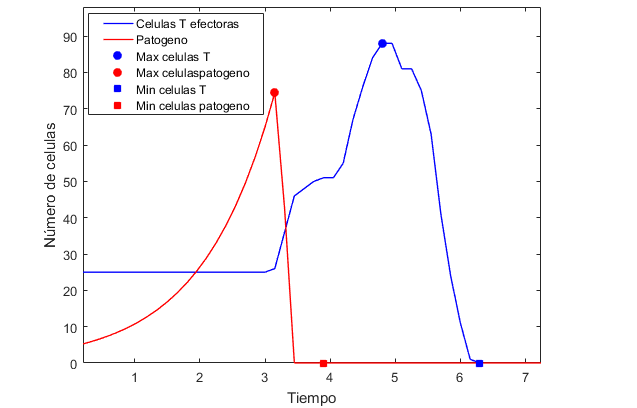
\includegraphics[width=0.5\textwidth]{Imagenes/RedNeuronal/micro}}
		& \subfloat[Simulación: caso de intolerancia al patógeno en el modelo macroscópico. Parámetros: $\alpha = 3,5$, $\beta = 0,29$, $k = 0,3$, $\lambda = 0,9$, $P_m = 0$.]{
			\label{fig:red_macro}
			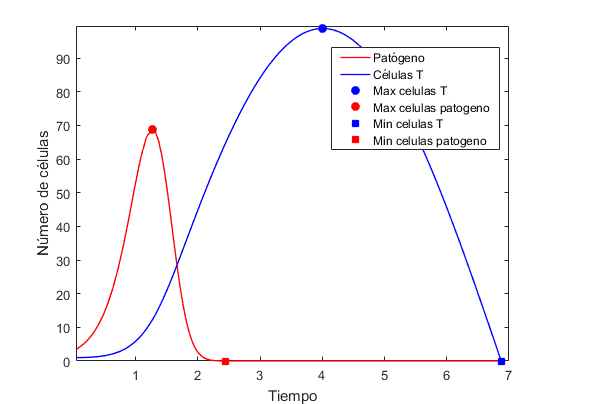
\includegraphics[width=0.5\textwidth]{Imagenes/RedNeuronal/macro}}\\
	\end{tabular}
	\caption{Ejemplo con simulaciones del modelo microscópico y macroscópico con los valores de los parámetros predichos por la red neuronal. Casos de intolerancia al patógeno.}%\label{foo}
\end{figure}



%\begin{figure}[t]
%	\centering
%	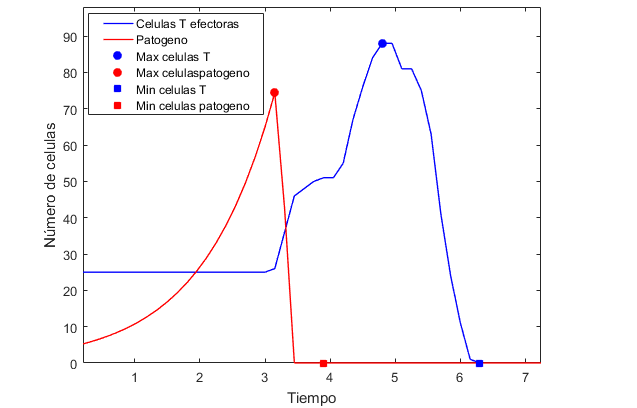
\includegraphics[width=0.7\textwidth]{Imagenes/RedNeuronal/micro}
%	\caption{Simulación: distintas poblaciones de células T con distintas afinidades al patógeno. Clon subdominante. Los parámetros son los mismos que se exponen en la Tabla \ref{tabla:param}, excepto: $\lambda_{Tp}^{clon_2} = 10^{-5}$.}
%	\label{fig:red_micro}
%\end{figure}













\chapter{Conclusiones y Trabajo Futuro}
\label{cap:conclusiones}

%Conclusiones del trabajo y líneas de trabajo futuro.

%Antes de la entrega de actas de cada convocatoria, en el plazo que se indica en el calendario de los trabajos de fin de máster, el estudiante entregará en el Campus Virtual la versión final de la memoria en PDF. En la portada de la misma deberán figurar, como se ha señalado anteriormente, la convocatoria y la calificación obtenida. Asimismo, el estudiante también entregará todo el material que tenga concedido en préstamo a lo largo del curso.

Tras la lectura de este documento hemos podido comprobar que las matemáticas pueden convertirse en herramientas muy potentes también fuera de su ámbito más teórico, algo que aún las enriquece más. Concretamente, las colaboraciones con biólogos cada vez son más frecuentes y, a pesar de ser ciencias muy distintas, se han obtenido resultados relevantes como el que describíamos a lo largo de estas páginas. Aún son numerosas las preguntas que quedan por resolver en el campo de la biología, es precisamente en esos puntos donde las matemáticas, gracias a su poder de abstracción y simplificación, pueden formular modelos que no solo reproduzcan hechos observados, sino que infieran nuevo conocimiento. Estas nuevas vías de investigación permiten, en muchos casos, avanzar en el estudio de una línea de pensamiento y descartar otras, dando cabida al progreso científico.

Los modelos propuestos en los Capítulos \ref{cap:descripcionTrabajo} y \ref{cap:modeloMacroscopico} se presentan como posibles explicaciones a un mecanismo biológico aún por determinar, como es la dinámica de población de las células T durante una infección aguda. Ambos modelos constituyen modelos robustos, flexibles y bien fundamentados, pues sus hipótesis las establecen evidencias biológicas. Gracias a estos modelos somos capaces de reproducir y predecir el comportamiento de las células T durante una infección aguda en distintas situaciones, sin necesidad de costosos experimentos ni un laboratorio, y desde dos puntos de vista diferentes, el microscópico y el macroscópico. Pero, sin duda, una de las características más importantes de estos modelos es que no son modelos cerrados, ambos están abiertos a la inclusión de nuevo conocimiento biológico. 

Otra de las cuestiones que aún busca respuesta es la planteada en el Capítulo \ref{cap:redNeuronal}. En este se buscaba establecer una correspondencia entre los parámetros de los dos modelos vistos en los capítulos anteriores. En este capítulo se detalla una primera aproximación para la resolución de esta compleja cuestión. Los resultados obtenidos por la red neuronal no son despreciables, pero aún insuficientes para poder deducir una correspondencia formal entre ambos modelos. Es por ello que queda a la espera de nuevo estudio e investigación.



%%%%%%%%%%%%%%%%%%%%%%%%%%%%%%%%%%%%%%%%%%%%%%%%%%%%%%%%%%%%%%%%%%%%%%%%%%%
% Si el TFM se escribe en inglés, comentar las siguientes líneas 
% porque no es necesario incluir nuevamente las Conclusiones en inglés
\begin{otherlanguage}{english}
\chapter{Introduction}
\label{cap:introduction}



The year 2018 was proclaimed International Year of Mathematical Biology by two scientific societies: the European Mathematical Society (EMS) and the European Society for Mathematical and Theoretical Biology (ESMTB). This celebration intended to highlight the importance of the applications of mathematics to biology and life sciences and to encourage their interaction\footnote{\url{https://www.icmat.es/divulgacion/Material_Divulgacion/miradas_matematicas/06.pdf}}. Today, life sciences are increasingly using mathematics, ranging from the use of dynamic systems and statistics to population and disease spread models. In this context, models play an important role, as they are simplified representations of the structure and functioning of a given biological system or process, using mathematical language to express the relationships between variables\footnote{\url{http://www.blogsanidadanimal.com/2018-el-ano-internacional-de-la-biologia-matematica/}}. The appropriate use of models allows us to advance beyond what mere intuition suggests and provides us with useful information that would otherwise be difficult to collect, either because of the high economic cost of the experiments, the time it takes to carry them out or the amount of data to be examined, among other reasons. But it is not only experts who benefit from the simplifying power of mathematical models. During the current COVID-19 health crisis, mathematical models have been used to predict the spread of the virus and to inform society of the risk of this pandemic\footnote{Mathematical models on COVID-19 growth curve in \textit{The Washington Post}: \url{https://www.washingtonpost.com/graphics/2020/world/corona-simulator/}}. 



Throughout this document, we will focus on the field of immunology. It is interesting to note that the cells that make up the immune system are not regulated by a coordinating organ \citep{arias2016emergent}. Immune cells move freely through the body, each living an independent life. However, they are capable of displaying collective behaviour, as is the case with the response to infectious agents. In this defensive function, T cells play a very important role. When an infection is detected, the population of this type of cells grows by several orders of magnitude in a few days and, once the infectious agent has disappeared, population levels are restored through the suicide (apoptosis) of a large part of the population generated. The decision mechanism between division or apoptosis taken by T cells during the immune response has many open questions as yet. In the following chapters, we will present two mathematical models, based on differential equations, which attempt to shed light on this phenomenon. The first one, which can be seen in Chapter \ref{cap:descripcionTrabajo}, deals with this issue from a microscopic point of view. That is, it proposes a decision algorithm implemented by each cell. Meanwhile, the equations of the second model, set out in Chapter \ref{cap:modeloMacroscopico}, describe the dynamic behaviour of the entire population of T cells, based on two main characteristics attributed to that population: elasticity and inertia. In both cases, numerical simulations of these models are performed. These simulations represent different situations that can occur during infection. Among them, it is interesting to distinguish between the situation of intolerance to the pathogen, when the immune cells manage to control the infection and eliminate the infectious agent, or the situation of tolerance to the pathogen, in which it is the latter who ends up taking control of the organism. 

The situation when we have populations of T cells with different affinities to the pathogen is also discussed there. The relationship between the properties of both models (microscopic and macroscopic) is an interesting issue, which is addressed in the last chapter (Chapter \ref{cap:redNeuronal}). As we will see, both give rise to results that are not only compatible but complementary. 



\section{Objectives}


This Final Project focuses on the study of the population dynamics of T cells in the face of acute infection and, more specifically, on the study of two mathematical models that aim to respond to the mechanisms that govern this behaviour.

To carry out this project, the following objectives were set:

\begin{itemize}
	
	\item A review of basic facts about the immune system, focusing on the role that T cells play during an \textit{immune response}.
	
	\item Motivation and analysis of the mathematical models detailed in this document and their relevance in the field of biology.
	
	\item Implementation of the code needed to simulate different T cell behaviours based on these models and analysis of these behaviours. 
	
	\item Obtaining a first approximation to establish a correspondence between the parameters of the two models studied. 
\end{itemize}

\section{Work plan}

To achieve the previous objectives, various milestones were established throughout the academic year. The first months were devoted to a prior review of the underlying biological concepts. These included basic notions about the immune system and a more detailed study of T cell behaviour. This constitutes a fundamental part of the work, as the models cannot be fully understood if they are not looked at in the context of the biological problem to which they are trying to respond. Once the biological basis was established, the study of the models could begin. The first one to be studied was the microscopic model shown in \cite{JTB}. Different simulations of the model were established, which would complement the theoretical results previously seen. The second model, the macroscopic one \citep{arias2015growth}, was later studied.

Once both models had been reviewed and the corresponding simulations had been carried out, the possibility was opened up of trying to establish a correspondence between the parameters of both models by implementing a neural network. Addressing this last question constitutes the last part of this memoir.


\section{Document structure}

This work is divided into four parts, which share a common purpose, the study of T cells and their population dynamics during an acute infection. 

\begin{enumerate}
	\item The background of the document is covered in Chapter \ref{cap:estadoDeLaCuestion}. In particular, Section \ref{sec:cuestInmuno} reviews basic notions of immunology, which allows the reader to proceed through the following chapters without any terminological impediment, as far as biological issues are concerned. This section is intended to give a very basic overview of the immune system. It starts with the simplest mechanisms, referring to the \textit{innate immune system} (Section \ref{sub:sistInmInnato}), to the most complex ones, referring to the \textit{adaptive immune system} (Section \ref{sub:sistInmAdap}). The aspects of the immune response involving T cells, such as their activation and performance or immune memory, are discussed in more detail (Section \ref{Tcell}).
	
	Furthermore, Section \ref{sec:coop} deals with the role of mathematical models in the field of biology. Specifically, in Section \ref{cuestionAmodelizar}, we focus on the case of our study, the different mathematical models formulated for the dynamics of T cells during an acute infection. 
	
	\item The theoretical framework of the proposed microscopic model for the problem of deciding between T cell division and apoptosis is presented in Chapter \ref{cap:descripcionTrabajo}. In Section \ref{sec:hip_bio} the biological hypotheses on which the model is based are detailed. Those hypotheses make use of well-known facts in the field of biology. The model itself can be seen in Section \ref{sec:modelo}, which contains the notation that will be followed by the rest of the document and the first-order differential equations that give rise to the algorithm. The last section of this chapter, Section \ref{sec:modeloPatCelT}, introduces a differential equation for the population dynamics of the pathogen and its relationship to the number of available T cells. The equation establishes the interaction between the two populations.
		
	In Chapter \ref{cap:simulaciones} the simulations corresponding to a simplified case of the previous model are presented (Section \ref{sec:modelo_simplif}) and the basic details of its implementation are explained (Section \ref{sec:implem_pseudo}). The results of the simulations are described in Section \ref{sec:simulacionesMicro}. These simulations correspond to cases of intolerance and tolerance to the pathogen (Sections \ref{sim:intoler} and \ref{sim:toler}, respectively), as well as the case of immune response when populations of T cells with different affinities to the pathogen are present (Section \ref{sim:difPoblacionesT}).
	
	\item The macroscopic model is then studied in Chapter \ref{cap:modeloMacroscopico}. The second-order differential equations of this model govern the population dynamics of T cells and the pathogen collectively, unlike the microscopic model, whose algorithm was defined for each individual cell. This model is based on two proposed characteristics of the T cell population behaviour during an immune response: elasticity and inertia (Section \ref{sec:iner_elast}). 
	
	In addition to proposing a theoretical model, numerical simulations of the corresponding equations are also carried out in Section \ref{sec:simu_macro}. These include the cases of intolerance and tolerance to the pathogen (Sections \ref{sub:simMacroIntoler} and \ref{sub:simMacroToler}, respectively) and, for the macroscopic non-dimensional model, the relevance of the value of two key parameters in the regions of tolerance and intolerance is studied (Section \ref{sub:reg_tolerIntolerMacro}).

	\item Then, after studying the models proposed in Chapters \ref{cap:descripcionTrabajo} and \ref{cap:modeloMacroscopico}, and after comparing their results, a parameter correspondence is sought between both models in Chapter \ref{cap:redNeuronal}. For this purpose, a neural network which is capable of performing ``the inverse function'' to the code referring to the simulations of the macroscopic model is implemented. That is to say, given the results of a simulation, the network can predict the value of the parameters necessary to obtain that same result. The construction of the dataset and the implementation of the network can be seen in the Section \ref{sec:conjDatos_entreRed}. The results obtained and an example of execution, using as input the results of a simulation of the microscopic model, can be seen in the Section \ref{sec:resultadoRed}.
	

\end{enumerate}

Finally, Chapter \ref{cap:conclusions} offers a brief summary of the work carried out. To complement the project, the main code of the model simulations (both those of Chapter \ref{cap:simulaciones} and \ref{cap:modeloMacroscopico}) has been included in Appendix \ref{Appendix:A}.


\chapter{Conclusions and Future Work}
\label{cap:conclusions}

The studies collected in this document show the usefulness of mathematical methods in proposing models that not only reproduce observed facts, but are also capable of suggesting explanations for them and make it possible to formulate predictions that can be verified, or discarded, experimentally. 


The models proposed in Chapters \ref{cap:descripcionTrabajo} and \ref{cap:modeloMacroscopico} are presented as possible explanations to a biological mechanism of great interest and only partially known, such as the population dynamics of T cells during an acute infection. Both models are well-founded, as their hypotheses are based on biological evidence. Thanks to these models we can reproduce and predict the behaviour of T cells during acute infection in different situations by varying the value of their parameters, without the need for expensive experiments and from two different points of view, the microscopic and the macroscopic. On the other hand, both are models open to the inclusion of new biological knowledge. 


From the microscopic model, we highlight its contrast to the hypothesis that the life of a T cell is determined by the \textit{antigenic stimulation} received during its activation. In this way, the cells generated in the \textit{clonal expansion} would have very limited control over their choice between division or apoptosis. However, the proposed model states that the encounters of a T cell with the \textit{antigen} are transmitted to the daughter cells using membrane receptors, which are distributed during cell division. This allows new cells to integrate this knowledge with their own experience with the \textit{antigen}, enabling cells that share the same ancestor to make different decisions. This shows that the heterogeneity of decisions observed during an immune response can be explained by a deterministic algorithm and can be independently executed by the T cells. The response given by T cells is specific to an \textit{antigen}, but not to a pathogen\footnote{A specific \textit{antigen} may be present in several pathogens, which may be very heterogeneous in terms of growth rates or escape mechanisms from the \textit{immune response}.}. This explains the fact that the mechanisms of pathogen recognition are not detailed in the model, giving it the capacity to adapt to different infection strategies \citep{JTB}


Meanwhile, the macroscopic model observes the population dynamics of T cells (\textit{clonal expansion} and \textit{contraction}) collectively. It, therefore, models their behaviour using second-order differential equations, based on two population properties: elasticity and inertia. This model yields interesting results. Specifically, it proposes that the mechanism of identification of the target population of T cells is determined by the growth rate of the T cell. In other words, those populations that grow rapidly are considered to be pathogenic, while those with reduced growth rates are tolerated. This proposal is compatible with the paradoxical fact that slow growth is the avoidance strategy of some tumour cells or viruses such as hepatitis C \citep{arias2015growth}.


Another question that we consider particularly relevant is the one raised in Chapter \ref{cap:redNeuronal}. In this chapter, we sought to establish a correspondence between the parameters of the two models seen in the previous chapters, since both show compatible population behaviour. The microscopic model is characterized by representing explicit biological characteristics of the cells by means of structural parameters, whose value remains fixed during the simulation. However, the meaning of the parameters of the macroscopic model, referring to the characteristics of inertia and elasticity of the T cell population, lacks a clear biological meaning. Nevertheless, one of the advantages of this model is the reduced number of parameters it has. Therefore, finding a parameter correspondence between the two models would be very useful, for example, to determine the parameters of the microscopic model that correspond to a certain \textit{immune response}. In this way, the response could be simulated using the macroscopic model, whose parameters are easier to adjust and subsequently establish the corresponding parameters in the microscopic model, which are easily interpreted. A first approximation to the resolution of this complex question is detailed in Chapter \ref{cap:redNeuronal}. The results obtained by the neural network are promising, but still insufficient to deduce a formal correspondence between both models. We hope to deepen this study in the near future.



\end{otherlanguage}
%%%%%%%%%%%%%%%%%%%%%%%%%%%%%%%%%%%%%%%%%%%%%%%%%%%%%%%%%%%%%%%%%%%%%%%%%%%

%
% Bibliografía
%
% Si el TFM se escribe en inglés, editar TeXiS/TeXiS_bib para cambiar el
% estilo de las referencias
%---------------------------------------------------------------------
%
%                      configBibliografia.tex
%
%---------------------------------------------------------------------
%
% bibliografia.tex
% Copyright 2009 Marco Antonio Gomez-Martin, Pedro Pablo Gomez-Martin
%
% This file belongs to the TeXiS manual, a LaTeX template for writting
% Thesis and other documents. The complete last TeXiS package can
% be obtained from http://gaia.fdi.ucm.es/projects/texis/
%
% Although the TeXiS template itself is distributed under the 
% conditions of the LaTeX Project Public License
% (http://www.latex-project.org/lppl.txt), the manual content
% uses the CC-BY-SA license that stays that you are free:
%
%    - to share & to copy, distribute and transmit the work
%    - to remix and to adapt the work
%
% under the following conditions:
%
%    - Attribution: you must attribute the work in the manner
%      specified by the author or licensor (but not in any way that
%      suggests that they endorse you or your use of the work).
%    - Share Alike: if you alter, transform, or build upon this
%      work, you may distribute the resulting work only under the
%      same, similar or a compatible license.
%
% The complete license is available in
% http://creativecommons.org/licenses/by-sa/3.0/legalcode
%
%---------------------------------------------------------------------
%
% Fichero  que  configura  los  parámetros  de  la  generación  de  la
% bibliografía.  Existen dos  parámetros configurables:  los ficheros
% .bib que se utilizan y la frase célebre que aparece justo antes de la
% primera referencia.
%
%---------------------------------------------------------------------


%%%%%%%%%%%%%%%%%%%%%%%%%%%%%%%%%%%%%%%%%%%%%%%%%%%%%%%%%%%%%%%%%%%%%%
% Definición de los ficheros .bib utilizados:
% \setBibFiles{<lista ficheros sin extension, separados por comas>}
% Nota:
% Es IMPORTANTE que los ficheros estén en la misma línea que
% el comando \setBibFiles. Si se desea utilizar varias líneas,
% terminarlas con una apertura de comentario.
%%%%%%%%%%%%%%%%%%%%%%%%%%%%%%%%%%%%%%%%%%%%%%%%%%%%%%%%%%%%%%%%%%%%%%
\setBibFiles{%
biblio%
}

%%%%%%%%%%%%%%%%%%%%%%%%%%%%%%%%%%%%%%%%%%%%%%%%%%%%%%%%%%%%%%%%%%%%%%
% Definición de la frase célebre para el capítulo de la
% bibliografía. Dentro normalmente se querrá hacer uso del entorno
% \begin{FraseCelebre}, que contendrá a su vez otros dos entornos,
% un \begin{Frase} y un \begin{Fuente}.
%
% Nota:
% Si no se quiere cita, se puede eliminar su definición (en la
% macro setCitaBibliografia{} ).
%%%%%%%%%%%%%%%%%%%%%%%%%%%%%%%%%%%%%%%%%%%%%%%%%%%%%%%%%%%%%%%%%%%%%%

%
%\setCitaBibliografia{
%\begin{FraseCelebre}
%\begin{Frase}
%  Y así, del mucho leer y del poco dormir, se le secó el celebro de
%  manera que vino a perder el juicio.\\ 
%  \textcolor{red}{(modificar en Cascaras$\backslash$bibliografia.tex)}
%\end{Frase}
%\begin{Fuente}
%  Miguel de Cervantes Saavedra
%\end{Fuente}
%\end{FraseCelebre}
%}

%%
%% Creamos la bibliografia
%%
\makeBib

% Variable local para emacs, para  que encuentre el fichero maestro de
% compilación y funcionen mejor algunas teclas rápidas de AucTeX

%%%
%%% Local Variables:
%%% mode: latex
%%% TeX-master: "../Tesis.tex"
%%% End:



% Apéndices
\appendix
\chapter{Código de las simulaciones}
\label{Appendix:A}

En este apéndice se expone el código utilizado para las simulaciones de los dos modelos vistos en este trabajo, el microscópico y el macroscópico, correspondientes al Capítulo \ref{cap:simulaciones} y Capítulo \ref{cap:modeloMacroscopico}, respectivamente. El código, realizado en Matlab, sigue la misma notación que se establece en los capítulos correspondientes.

\section{Código referente al Capítulo \ref{cap:simulaciones}}
\label{sec:codigoMicro}
En esta sección se expone el código principal de las simulaciones vistas en el Capítulo \ref{cap:simulaciones}. El código que sigue corresponde a la Figura \ref{fig:intolerance} donde puede verse el caso de intolerancia al \textit{patógeno}. Para la simulación del caso de tolerancia, que aparece en la Figura \ref{fig:tolerance}, el código es exactamente el mismo aunque varía el valor de los parámetros, como ya se expuso en la correspondiente figura. 

Para el caso de las figuras correspondientes a varias poblaciones de células T (Figura \ref{fig:tresClones} - Figura \ref{fig:unClon}) la idea que subyace es similar, simplemente se añadieron los correspondientes parámetros y estructuras para guardar la acción de cada una de las poblaciones de células T. 

Las funciones \textit{sys\_4\_1\_sol} y \textit{sys\_4\_2\_sol} dan el resultado de la solución explícita de los sistemas \ref{sist9_simplif} y \ref{sist15_simplif}, respectivamente, evaluada en los parámetros que se pasan a la función. La estructura \textit{t\_cell\_matrix} es una matriz que almacena en cada fila una célula de la población y cuyas columnas guardan los parámetros correspondientes a esa célula (su tipo, condiciones iniciales y el tiempo que le queda para completar la fase de ciclo o apoptosis, en caso de que se encuentre en alguna de ellas). 

\lstinputlisting[language=Matlab]{Codigo/Cap_4_Tolerancia_intolerancia/intolerance_sys_4_1.m}


\section{Código referente al Capítulo \ref{cap:modeloMacroscopico}}
\label{sec:codigoMacro}

Es el turno de ver el código correspondiente al modelo macroscópico. En esta ocasión no disponíamos de un sistema de ecuaciones diferenciales con solución explícita, por lo que tenemos una simulación numérica mediante el uso de la función \textit{ode\_45}\footnote{\url{https://www.mathworks.com/help/matlab/ref/ode45.html}} de Matlab. A continuación podemos ver el código referente a la Figura \ref{fig:macro_intolerance}. En la línea $33$ se incluye la condición $T \geq 0$.

Para simular la Figura \ref{fig:macro_tolerance}, correspondiente al caso de tolerancia, se tomó el Sistema \ref{sist_macro_nod}, el código sigue la misma estructura aunque las ecuaciones que vemos en las líneas 24 y 25 sufren una ligera modificación: los parámetros $k$ y $\lambda$ desaparecen y se sustituyen $a$ ($\alpha$) y $b$ ($\beta$) por los correspondientes $a\_star$ ($\alpha ^{*}$) y $b\_star$ ($\beta ^{*}$) del Sistema \ref{sist_macro_nod}. 

\lstinputlisting[language=Matlab]{Codigo/Cap_5_Modelo_macroscopico/macro_intolerance.m}


Veamos ahora el código de la Figura \ref{fig:macro_toler_intoler}: En este caso queríamos hacer simulaciones variando el valor de los parámetros $\alpha ^{*}$ y $\beta ^{*}$. Para ello tenemos un código que va recorriendo valores en el intervalo $[0, 2'5]$ y llamando con cada par de valores $\alpha ^{*}$ y $\beta ^{*}$ a la función \textit{macro\_nond\_toler\_into} que realiza la simulación del Sistema \ref{sist_macro_nod} y devuelve si hay tolerancia o intolerancia midiendo la cantidad de \textit{patógeno} que queda al final de la simulación. Teniendo en cuenta el resultado, se pinta un rombo rojo si estamos ante un caso de tolerancia o verde en caso de intolerancia al \textit{patógeno}.

\lstinputlisting[language=Matlab]{Codigo/Cap_5_Modelo_macroscopico/script_nond_alphaBeta.m}


\lstinputlisting[language=Matlab]{Codigo/Cap_5_Modelo_macroscopico/macro_nond_toler_into.m}
%\chapter{Título del Apéndice B}
\label{Appendix:Key2}

%\include{Apendices/appendixC}
%\include{...}
%\include{...}
%\include{...}
\backmatter



%
% Índice de palabras
%

% Sólo  la   generamos  si  está   declarada  \generaindice.  Consulta
% TeXiS.sty para más información.

% En realidad, el soporte para la generación de índices de palabras
% en TeXiS no está documentada en el manual, porque no ha sido usada
% "en producción". Por tanto, el fichero que genera el índice
% *no* se incluye aquí (está comentado). Consulta la documentación
% en TeXiS_pream.tex para más información.
\ifx\generaindice\undefined
\else
%%---------------------------------------------------------------------
%
%                        TeXiS_indice.tex
%
%---------------------------------------------------------------------
%
% TeXiS_indice.tex
% Copyright 2009 Marco Antonio Gomez-Martin, Pedro Pablo Gomez-Martin
%
% This file belongs to TeXiS, a LaTeX template for writting
% Thesis and other documents. The complete last TeXiS package can
% be obtained from http://gaia.fdi.ucm.es/projects/texis/
%
% This work may be distributed and/or modified under the
% conditions of the LaTeX Project Public License, either version 1.3
% of this license or (at your option) any later version.
% The latest version of this license is in
%   http://www.latex-project.org/lppl.txt
% and version 1.3 or later is part of all distributions of LaTeX
% version 2005/12/01 or later.
%
% This work has the LPPL maintenance status `maintained'.
% 
% The Current Maintainers of this work are Marco Antonio Gomez-Martin
% and Pedro Pablo Gomez-Martin
%
%---------------------------------------------------------------------
%
% Contiene  los  comandos  para  generar  el índice  de  palabras  del
% documento.
%
%---------------------------------------------------------------------
%
% NOTA IMPORTANTE: el  soporte en TeXiS para el  índice de palabras es
% embrionario, y  de hecho  ni siquiera se  describe en el  manual. Se
% proporciona  una infraestructura  básica (sin  terminar)  para ello,
% pero  no ha  sido usada  "en producción".  De hecho,  a pesar  de la
% existencia de  este fichero, *no* se incluye  en Tesis.tex. Consulta
% la documentación en TeXiS_pream.tex para más información.
%
%---------------------------------------------------------------------


% Si se  va a generar  la tabla de  contenidos (el índice  habitual) y
% también vamos a  generar el índice de palabras  (ambas decisiones se
% toman en  función de  la definición  o no de  un par  de constantes,
% puedes consultar modo.tex para más información), entonces metemos en
% la tabla de contenidos una  entrada para marcar la página donde está
% el índice de palabras.

\ifx\generatoc\undefined
\else
   \addcontentsline{toc}{chapter}{\indexname}
\fi


% Generamos el índice
\printindex

% Variable local para emacs, para  que encuentre el fichero maestro de
% compilación y funcionen mejor algunas teclas rápidas de AucTeX

%%%
%%% Local Variables:
%%% mode: latex
%%% TeX-master: "./tesis.tex"
%%% End:

\fi

%
% Lista de acrónimos
%

% Sólo  lo  generamos  si  está declarada  \generaacronimos.  Consulta
% TeXiS.sty para más información.


\ifx\generaacronimos\undefined
\else
%---------------------------------------------------------------------
%
%                        TeXiS_acron.tex
%
%---------------------------------------------------------------------
%
% TeXiS_acron.tex
% Copyright 2009 Marco Antonio Gomez-Martin, Pedro Pablo Gomez-Martin
%
% This file belongs to TeXiS, a LaTeX template for writting
% Thesis and other documents. The complete last TeXiS package can
% be obtained from http://gaia.fdi.ucm.es/projects/texis/
%
% This work may be distributed and/or modified under the
% conditions of the LaTeX Project Public License, either version 1.3
% of this license or (at your option) any later version.
% The latest version of this license is in
%   http://www.latex-project.org/lppl.txt
% and version 1.3 or later is part of all distributions of LaTeX
% version 2005/12/01 or later.
%
% This work has the LPPL maintenance status `maintained'.
% 
% The Current Maintainers of this work are Marco Antonio Gomez-Martin
% and Pedro Pablo Gomez-Martin
%
%---------------------------------------------------------------------
%
% Contiene  los  comandos  para  generar  el listado de acrónimos
% documento.
%
%---------------------------------------------------------------------
%
% NOTA IMPORTANTE:  para que la  generación de acrónimos  funcione, al
% menos  debe  existir  un  acrónimo   en  el  documento.  Si  no,  la
% compilación  del   fichero  LaTeX  falla  con   un  error  "extraño"
% (indicando  que  quizá  falte  un \item).   Consulta  el  comentario
% referente al paquete glosstex en TeXiS_pream.tex.
%
%---------------------------------------------------------------------


% Redefinimos a español  el título de la lista  de acrónimos (Babel no
% lo hace por nosotros esta vez)

\def\listacronymname{Lista de acrónimos}

% Para el glosario:
% \def\glosarryname{Glosario}

% Si se  va a generar  la tabla de  contenidos (el índice  habitual) y
% también vamos a  generar la lista de acrónimos  (ambas decisiones se
% toman en  función de  la definición  o no de  un par  de constantes,
% puedes consultar config.tex  para más información), entonces metemos
% en la  tabla de contenidos una  entrada para marcar  la página donde
% está el índice de palabras.

\ifx\generatoc\undefined
\else
   \addcontentsline{toc}{chapter}{\listacronymname}
\fi


% Generamos la lista de acrónimos (en realidad el índice asociado a la
% lista "acr" de GlossTeX)

\printglosstex(acr)

% Variable local para emacs, para  que encuentre el fichero maestro de
% compilación y funcionen mejor algunas teclas rápidas de AucTeX

%%%
%%% Local Variables:
%%% mode: latex
%%% TeX-master: "../Tesis.tex"
%%% End:

\fi

%
% Final
%
%%---------------------------------------------------------------------
%
%                      fin.tex
%
%---------------------------------------------------------------------
%
% fin.tex
% Copyright 2009 Marco Antonio Gomez-Martin, Pedro Pablo Gomez-Martin
%
% This file belongs to the TeXiS manual, a LaTeX template for writting
% Thesis and other documents. The complete last TeXiS package can
% be obtained from http://gaia.fdi.ucm.es/projects/texis/
%
% Although the TeXiS template itself is distributed under the 
% conditions of the LaTeX Project Public License
% (http://www.latex-project.org/lppl.txt), the manual content
% uses the CC-BY-SA license that stays that you are free:
%
%    - to share & to copy, distribute and transmit the work
%    - to remix and to adapt the work
%
% under the following conditions:
%
%    - Attribution: you must attribute the work in the manner
%      specified by the author or licensor (but not in any way that
%      suggests that they endorse you or your use of the work).
%    - Share Alike: if you alter, transform, or build upon this
%      work, you may distribute the resulting work only under the
%      same, similar or a compatible license.
%
% The complete license is available in
% http://creativecommons.org/licenses/by-sa/3.0/legalcode
%
%---------------------------------------------------------------------
%
% Contiene la última página
%
%---------------------------------------------------------------------


% Ponemos el marcador en el PDF
\ifpdf
   \pdfbookmark{Fin}{fin}
\fi

\thispagestyle{empty}\mbox{}

Este texto se puede encontrar en el fichero Cascaras/fin.tex. Si deseas eliminarlo, basta con comentar la línea correspondiente al final del fichero TFMTeXiS.tex.

\vspace*{4cm}

\small

\hfill \emph{--¿Qué te parece desto, Sancho? -- Dijo Don Quijote --}

\hfill \emph{Bien podrán los encantadores quitarme la ventura,}

\hfill \emph{pero el esfuerzo y el ánimo, será imposible.}

\hfill 

\hfill \emph{Segunda parte del Ingenioso Caballero} 

\hfill \emph{Don Quijote de la Mancha}

\hfill \emph{Miguel de Cervantes}

\vfill%space*{4cm}

\hfill \emph{--Buena está -- dijo Sancho --; fírmela vuestra merced.}

\hfill \emph{--No es menester firmarla -- dijo Don Quijote--,}

\hfill \emph{sino solamente poner mi rúbrica.}

\hfill 

\hfill \emph{Primera parte del Ingenioso Caballero} 

\hfill \emph{Don Quijote de la Mancha}

\hfill \emph{Miguel de Cervantes}


\newpage
\thispagestyle{empty}\mbox{}

\newpage

% Variable local para emacs, para  que encuentre el fichero maestro de
% compilación y funcionen mejor algunas teclas rápidas de AucTeX

%%%
%%% Local Variables:
%%% mode: latex
%%% TeX-master: "../Tesis.tex"
%%% End:

%\end{otherlanguage}
\end{document}
